\documentclass[12pt,letterpaper,spanish]{article}

\makeatletter  %%%%%% modificacion macro (para puntos en el indice)
\renewcommand*\l@section{\@dottedtocline{1}{1.5em}{2.3em}}
\renewcommand\@dotsep{0.8}
\makeatother %%%%%% fin modificacion macro 

\usepackage[utf8]{inputenc}
\usepackage[spanish]{babel}
\usepackage{times} %Para que salga en times
\usepackage{hyperref}
\hypersetup{colorlinks=true,allcolors=black}
\urlstyle{same}
\usepackage{hypcap}
\usepackage[breakable]{tcolorbox}
\usepackage{dirtytalk}
\usepackage{seqsplit}
\usepackage{wrapfig}
\usepackage{float}
\usepackage{fancyhdr}

 %%%%%%% Packages para hacer las citas
\usepackage[fixlanguage]{babelbib}
\selectbiblanguage{spanish}
\addto\captionsspanish{%
\def\bibname{Referencias}%
\def\tablename{Tabla}%
}
%%%%%%%%%%%%%%%%%%%%%%%%%%%%%%%%%%%%%%%%



\fancyhf{} % sets both header and footer to nothing
\renewcommand{\headrulewidth}{0pt}
% your new footer definitions here


\usepackage{graphicx}
\usepackage{caption}
\usepackage[left=3cm,right=2.5cm,top=3cm,bottom=2.5cm]{geometry}
\usepackage{pdfpages}
\usepackage{amsmath}
\usepackage{longtable}
\usepackage{subfigure} 
\usepackage{ragged2e}
\usepackage{multicol}
\usepackage{xcolor}
\usepackage{rotating}
\usepackage{xcolor}
\usepackage{sectsty}
\usepackage{glossaries}

%Estilo de la página
%\def\arraystretch{1.5}
\renewcommand{\baselinestretch}{1.15}


\chead{\thepage}
%\title{\hfill
\includegraphics[scale=0.6]{logo.png}\vspace{4em}\\
\title{
Pontificia Universidad Católica de Valparaíso\\
Facultad de Ingeniería\\
Escuela de Ingeniería Industrial\vspace{3em}\\
\textbf{Análisis relacional de la pobreza multidimensional en Chile}} %%%%%%%% TITULO INFORME
\author{\LARGE{por}\vspace{1em}\\
\textbf{\LARGE{Maximiliano Muñoz Leiva}}\vspace{1.5mm}\\
\textbf{\LARGE{Matías Negrete Oliva}}\vspace{1.5mm}\\
\textbf{\LARGE{Matías Rodríguez Urtubia}}\vspace{3em}\\
\LARGE{Informe final técnico}\vspace{2em}\\
\LARGE{Prof. Guía: Sebastián Cea Echenique}\vspace{1em}\\
\LARGE{Prof. Co-Guía: Carlos Erazo Jojot}\vspace{3em}}
\date{\LARGE{8 de julio, 2020}}
\begin{document}
\renewcommand{\listtablename}{Lista de Tablas}%%%%%%%%%%% cambio de nombre
\renewcommand{\listfigurename}{Lista de Figuras} %%%%%%% cambio de nombre


\maketitle
\thispagestyle{empty}
\pagestyle{fancy}
\setlength{\parindent}{1cm} %%%%%%%% sangría inicio cada párrafo
\setlength{\parskip}{1em}
%Inicio del documento como tal %%%%%%%%%%%%%%%%%%%%%%%%%%%%%%%%%%%%%%%%%%%%%%%%%%%%%%
%%%%%%%%%%
\newpage
\begin{center}%%%%%% inicio centrado índice, figuras, tablas
\tableofcontents
\clearpage
\listoffigures
\clearpage
%\listoftables
\clearpage
\end{center}%%%%%%% fin centrado índice, figuras, tablas
%%%%%%%%%%%%%%%%%%%%%%%%%%%%%%%%%%%%%%%%%%%%%%%%%%%%%%%%%%%%%%%%%%%%%%%%%%%%%%%%%%%%%

\section*{Resumen ejecutivo}\addcontentsline{toc}{section}{Resumen ejecutivo} % Max 2 paginas, 5 puntos
La sociedad chilena ha experimentado cambios evidentes en las últimas décadas, disminuyendo significativamente el porcentaje de personas en situación de pobreza por ingresos\footnote{Ver evolución pobreza Encuesta Casen 2006-2017 en \url{http://observatorio.ministeriodesarrollosocial.gob.cl/casen-multidimensional/casen/docs/Resultados_pobreza_Casen_2017.pdf}.}, como resultado del incremento sostenido de los ingresos promedio de los hogares y de las transferencias del Estado\footnote{Ver evolución ingresos de los hogares en \url{https://www.ine.cl/estadisticas/sociales/ingresos-y-gastos/encuesta-suplementaria-de-ingresos}.}. Esto no ha sido un fenómeno aislado, sino que constituye un proceso global de reducción de la pobreza y pobreza extrema\footnote{Ver evolución de pobreza y pobreza extrema en el Mundo 1990-2015 en \url{https://data.worldbank.org/indicator/SI.POV.UMIC?name_desc=false} y \url{https://data.worldbank.org/topic/poverty?name_desc=false} respectivamente.} que, a su vez, ha generado e impulsado la aparición de una gran clase media en Chile \cite{Candia2017RadiografiaPublica} y el Mundo\footnote{Ver evolución de la población de ingresos medios en el Mundo 1990-2018 en \url{https://data.worldbank.org/indicator/SP.POP.TOTL?locations=XP&name_desc=true}.}. A pesar de estos avances, se ha evidenciado un profundo malestar en los últimos años acompañado de crecientes demandas sociales\footnote{Ver noticias ONU en \url{https://news.un.org/es/story/2019/12/1466381}.}, que ha dejado de manifiesto que el problema debe entenderse como un fenómeno complejo.  

Desde las propuestas realizadas por Amartya Sen \cite{Sen1976Poverty:Measurement}, los esfuerzos por entender el fenómeno de la pobreza y contar con una medición nueva y apropiada de la misma se han intensificado. En 2007, Sabina Alkire y James Foster, de la Universidad de Oxford, realizaron una propuesta metodológica para medir la pobreza multidimensional de manera agregada, reflejando la prevalencia de la pobreza (cantidad de personas en situación de pobreza) y la distribución conjunta de las privaciones (probabilidad de experimentar carencias simultáneas) \cite{Alkire2007CountingMeasurement}. En 2010, Alkire y Santos tomaron elementos de esta metodología y desarrollaron el Índice de Pobreza Multidimensional (\textit{IPM}) del \textit{PNUD} \cite{Alkire2010AcuteCountries}  que sustituyó el Índice de Pobreza Humana (\textit{IPH}) que \textit{ONU} venía aplicando desde 1997. 

En 2015, el Ministerio de Desarrollo Social y Familia de Chile oficializó cambios metodológicos a los indicadores de pobreza, transitando de una concepción económica a un entendimiento multidimensional de la misma, que la reconoce como un fenómeno complejo. La metodología de la pobreza multidimensional actual recogió la propuesta de Alkire y Foster, desagregando la pobreza en 5 dimensiones (Educación; Salud; Trabajo y seguridad social; Vivienda y entorno; Redes y cohesión social), donde cada una agrupa tres carencias con ponderaciones específicas que al ser sumadas obtienen el indicador general de pobreza multidimensional (\textit{IPM}). En 2016, el sociólogo Pablo Beytía realizó un análisis relacional de la estructura interna de la pobreza multidimensional en base a la Encuesta Casen 2015 \cite{Beytia2016LaMultidimensional}, considerando las carencias del indicador de pobreza multidimensional como una red de correlaciones, es decir, una red de vínculos mutuos entre carencias. Pudo indagar en las dinámicas internas del fenómeno, observar patrones estructurales y calcular pesos estructurales de cada variable y de cada dimensión. 


Considerando el contexto actual de profundas transformaciones sociales, que también han transformado al concepto de familia \cite{OECD2011DoingChanging}, y con las nuevas metodologías para aproximarse holísticamente al fenómeno de la pobreza, el Observatorio Internacional de la Familia de Milán, a través del Programa de Ciencias para la Familia de la PUCV, se encuentra realizando un estudio que tiene por objeto comprender con mayor profundidad las relaciones existentes entre las características y las carencias de las familias. El presente estudio surge con el fin de ser un apoyo al trabajo desarrollado por el Programa de Ciencias para la Familia, mediante una aproximación relacional del análisis de la pobreza. 


La elaboración del estudio se dividió en tres etapas. La primera replicó el análisis relacional de la estructura interna de la pobreza multidimensional desarrollado por Beytía \cite{Beytia2016LaMultidimensional}, considerando esta vez los datos de la Encuesta Casen 2017. En la segunda etapa, a la muestra de hogares pobres multidimensionales se le aplicó la propiedad de descomponibilidad considerando el tipo de hogar, el número de personas que integran el hogar y la zona de residencia del hogar (rural o urbano). A los tipos de hogares se les efectuó un análisis relacional, y al resto de los subgrupos se les realizó un análisis tipológico de las carencias. También se hizo un análisis comparativo con el nivel de ingresos de los hogares. En la última etapa, se recopilaron proyecciones de índices socioeconómicos que permitieron proyectar el indicador de pobreza multidimensional en Chile. Adicionalmente, se realizó un análisis de sensibilidad de las ponderaciones de los indicadores locales del \textit{IPM} (carencias).





 


\newpage
\section{Definición del proyecto} %10 puntos
En esta sección se presenta la descripción del contexto organizacional, la descripción del equipo investigador, la formalización del problema, y el propósito, la justificación y el objetivo del proyecto. También se identifica el sistema de estudio, sus funciones incorporadas y las partes interesadas.

\subsection{Contexto organizacional}
El 6 de diciembre de 2018, en una iniciativa del Pontificio Instituto Teológico Juan Pablo II para las Ciencias del Matrimonio y la Familia, en cooperación con la Universidad Católica San Antonio de Murcia (UCAM) y el Centro Internacional de Estudios de la Familia (CISF) de Milán, se creó el Observatorio Internacional de la Familia, cuyo objetivo es analizar el rol que desempeñan las relaciones familiares en la pobreza de las personas\footnote{Ver más información en \url{https://www.vaticannews.va/es/vaticano/news/2018-12/vaticano-observatorio-internacional-familia-pobreza-relaciones.html} y \url{https://www.familymonitor.net/}.}. El Observatorio ha contactado a distintas instituciones académicas y centros de estudio, a los cuales les ha encargado la recopilación de datos nacionales fiables sobre la realidad de las familias en el mundo. Ofrecerá continuamente detalles de la evolución de las condiciones de las familias y comparará las dinámicas familiares en los distintos contextos culturales y políticos de los países, lo cual permitirá enriquecer el análisis de las distintas realidades familiares entendiendo sus complejidades\footnote{Ver información en \url{https://www.vaticannews.va/es/vaticano/news/2018-12/vaticano-observatorio-internacional-familia-pobreza-relaciones.html}.}. 

La primera etapa de la investigación incluyó países de Europa, África y América Latina, y su foco de estudio fue entender cómo la pobreza relacional y económica influye en las dinámicas familiares. El Programa de Ciencias para la Familia, de la Pontificia Universidad Católica de Valparaíso, fue la institución académica seleccionada para realizar la investigación en Chile, disponiendo un equipo interdisciplinario para abordar dicha tarea. El desarollo del presente proyecto fue realizado como una instancia de colaboración al trabajo de este equipo, el cual se encuentra iniciando la segunda etapa de investigación que finaliza en 2021. 

\subsection{Descripción organizacional}
El equipo investigador se encuentra constituido por el Director del proyecto y por diez investigadores. En la Figura \ref{equipoInv} se presenta el detalle de los integrantes del equipo con sus respectivas escuelas, institutos o facultades de origen:
\begin{figure}[H]
    \centering
        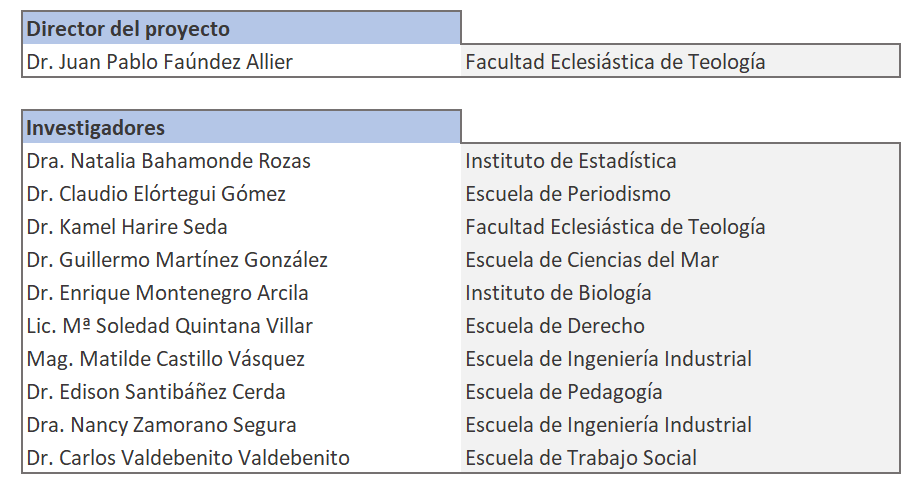
\includegraphics[height=8cm]{Heatmaps/EquipoInvestigador.png}
    \caption{Integrantes Comisión Investigadora. Fuente: Programa de Ciencias para la Familia.}
    \label{equipoInv}
\end{figure}
La diversidad de profesiones y áreas de estudio constituye una de las características principales de este equipo investigador, ya que provee distintas visiones y métodos para aproximarse al objeto de estudio que fue definido como un fenómeno complejo. 

\subsection{Formalización del problema}

En virtud de focalizar la investigación llevada a cabo por el Observatorio Internacional de la Familia, se ha formulado una serie de interrogantes, en cuyas respuestas se encuentra el cumplimiento del objetivo inicialmente planteado. La interrogante original del observatorio se puede resumir de la siguiente forma: \textbf{¿Cuál es el rol que desempeñan las relaciones familiares en la pobreza de las personas, desde la perspectiva económica y afectiva?}\footnote{Ver información en \url{https://www.vaticannews.va/es/vaticano/news/2018-12/vaticano-observatorio-internacional-familia-pobreza-relaciones.html}}. 

En la búsqueda de una premisa elaborada que responda a esta pregunta, la comisión de investigación de la PUCV busca desagregar la interrogante para ser abordada desde diferentes aproximaciones disciplinares.  En este contexto, nace el interés de la comisión en profundizar la comprensión de las dinámicas relacionales que surgen de la interacción entre los distintos elementos que componen el fenómeno de la pobreza, desde la perspectiva multidimensional. 

\textbf{ACA IRÁ MARCO TEÓRICO POBREZA MULTIDIMENSIONAL, Y DE LA APLICACIÓN DEL MODELO EN CHILE (5 DIMENSIONES Y SUS RESPECTIVAS CARENCIAS Y PONDERACIONES.}


(...)En consecuencia, el equipo de investigadores designados por el Programa de Ciencias para la Familia ha levantado los siguientes cuestionamientos:

\begin{itemize}

    \item ¿Cuáles son las propiedades de la pobreza multidimensional que surgen de la interacción entre los distintos tipos de carencias?

    \item ¿Existen características relacionales entre las carencias que son propias de los diferentes tipos de hogares?

    \item ¿Cómo afecta el número de miembros de cada hogar, su zona de residencia, y su nivel de ingresos en la conformación estructural de sus carencias?

    \item ¿Cuál sería la distribución de la pobreza multidimensional, si a las carencias relacionadas a la dimensión de Redes y cohesión social se les atribuyera la misma relevancia que al resto de las carencias?

    \item ¿Cómo se proyecta la pobreza multidimensional en Chile en el período de crisis sanitaria y social?

\end{itemize}

Ante la necesidad de la comisión de encontrar respuestas, el presente proyecto de investigación busca aportar con información valiosa que contribuya en la comprensión del fenómeno de la pobreza, realizando un estudio desde una perspectiva relacional, para luego complementarlo aplicando criterios de descomponibilidad. Se espera que en su realización se provea a la comisión de los elementos necesarios para el correcto entendimiento de la pobreza multidimensional en la realidad nacional, el cual eventualmente podría permitir focalizar adecuadamente los recursos de las futuras intervenciones sociales que la Iglesia Católica realice en Chile.

\subsection{Resultados esperados y criterios de aceptación}

%poner las hipótesis y criterios de aceptación

Los criterios de aceptación del estudio realizado se basan, en primera instancia, en la disposición de evidencia que permita aceptar o refutar una serie de afirmaciones que se plantean como respuestas posibles a las interrogantes enunciadas en la sección anterior. Estas afirmaciones pueden ser formalizadas en las siguientes hipótesis:

\begin{itemize}
    \item La aproximación al estudio de la pobreza multidimensional desde la perspectiva relacional permitiría profundizar en el entendimiento de las dinámicas relacionales; dinámicas que surgen de la interacción entre los distintos tipos de carencias. Se plantea la posibilidad de la existencia de factores relacionales que son inadvertidos desde la perspectiva analítica. 
    
    \item La aplicación de la propiedad de descomponibilidad\footnote{Partición de la muestra tomando en cuenta criterios que actúan como filtros de variedad.} al objeto del estudio (hogares pobres multidimensionales) permitiría identificar dinámicas relacionales particulares de cada subgrupo, las cuales estarían determinadas por ciertos factores externos\footnote{Los criterios de descomponibilidad definidos se basan en la clasificación de los factores externos.} a las carencias. Particularmente, se plantea que la diferenciación de los hogares según su estructura (tipos de hogares), según su zona de residencia (rural o urbana) y según su tamaño (número de integrantes) permitiría identificar dinámicas relacionales propias de los subconjuntos diferenciados. 

    \item Existe una relación entre la prevalencia de la pobreza multidimensional y el nivel de ingresos de los hogares pobres multidimensionales. Además, se puede identificar una relación lineal entre el nivel de ingresos y  la intensidad de la pobreza multidimensional (expresada en el índice de pobreza multidimensional \textit{IPM}). 


\end{itemize}  

En segunda instancia, los criterios de aceptación se refieren a la disposición de información que permita prever un escenario probable de la situación actual del fenómeno de la pobreza multidimensional en Chile, así como también del escenario de distribución de la pobreza multidimensional, si se le atribuyera la misma relevancia a las carencias de la dimensión \textit{Redes y cohesión social} que la atribuida al resto de las carencias, para el cálculo del \textit{IPM}.



 













\subsection{Identificación del sistema en estudio}
Si bien el objeto de estudio de este proyecto es la pobreza, esta no se entiende por sí sola, ya que requiere del componente humano para manifestarse. El sistema en estudio, en consecuencia, corresponde a los grupos familiares circunscritos dentro de Chile, cuyas características estructurales determinan la manifestación o no de la pobreza. Resulta relevante recordar que para efectos prácticos y en coherencia con la metodología utilizada, la unidad de análisis es el hogar. Por lo tanto, en este proyecto el hogar constituye la aproximación hacia el estudio de las familias en Chile.

Desde una perspectiva sistémica se entenderá que las familias corresponden a un sistema abierto, donde cada una es un grupo organizado de personas, con identidad propia y en constante interacción, que forman un entramado de relaciones \cite{I.Espinal.2006ElFamilia}. Estas y otras características como la auto-organización, las propiedades emergentes, la retroalimentación, la impredecibilidad y la adaptación, dan cuenta de que la familia también se puede considerar como un sistema complejo.



\newpage
\section{Metodología de ejecución del proyecto} % 10 puntos

La metodología empleada en el desarrollo del proyecto ``Análisis Relacional de la Pobreza Multidimensional en Chile"  se dividió en 3 etapas principales, cada una de las cuales estuvo orientada a comprobar un conjunto determinado de hipótesis y a contribuir en la búsqueda de respuestas a la problemática planteada en la definición del proyecto.

\begin{figure}[H]
    \centering
    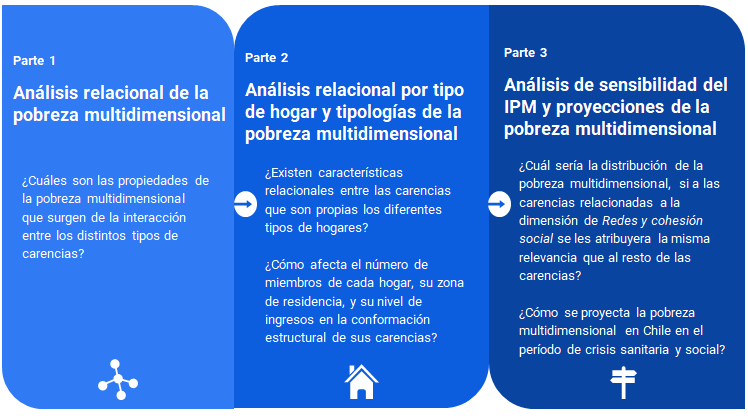
\includegraphics[width=\textwidth]{Max/intro_metodologia.png}
    \caption{División del trabajo metodológico y problemáticas planteadas. Fuente: elaboración propia.}
    \label{intro_metodologia}
\end{figure}






\newpage
\subsection{Metodología análisis relacional de la pobreza multidimensional}

La metodología descrita a continuación tiene por objetivo estudiar las dinámicas relacionales entre las carencias componentes de la pobreza multidimensional. Es decir, en su implementación se buscará entender, desde un enfoque no analítico, la forma en que los distintos tipos de carencias interactúan para conformar el estado de pobreza multidimensional de los hogares en Chile.


\begin{enumerate}
\item \textbf{Obtención de variables} 

Cada hogar se encuentra caracterizado por un conjunto de 15 atributos\footnote{Los atributos que indican la existencia de una carencia son compartidos por todos los miembros que componen un hogar, indistintamente de si alguno de ellos no la posee particularmente.} que indican la existencia o no existencia de cada una de las 15 carencias descritas en el modelo de pobreza multidimensional de 5 dimensiones\footnote{Modelo aplicado en la encuesta CASEN 2017.}. El criterio aplicado para el cálculo del indicador de cada una estas carencias se encuentra disponible en la documentación que dispone el Ministerio de Desarrollo Social y Familia (fig. \ref{tabla_indicadores}; Anexos - fig.\ref{criterios}), y determina la asignación de los valores 1 y 0, en caso de la existencia y la no existencia cada carencia. 


Las variables que requeridas para el análisis relacional corresponden a los indicadores de cada  una de las carencias que componen el índice de pobreza multidimensional (\textit{IPM}), para todos los hogares catalogados como pobres multidimensionales (es decir, aquellos con \textit{IPM} mayor o igual a 22.5\%). Estos indicadores, así como las clasificaciones de los hogares en situación de pobreza dimensional, se encuentran en la base de datos con los resultados de la encuesta CASEN 2017 que dispone el Ministerio de Desarrollo Social y Familia del Gobierno de Chile\footnote{En el documento anexo \ref{descripcion_base_datos} se dispone de una descripción extendida de la base de datos empleada, así como de los atributos asociados a la existencia de cada una de las carencias.}


De forma adicional, se define un conjunto de 5 variables para cada hogar pobre multidimensional de la muestra, cada una de las cuales representa un indicador agregado de las carencias que componen cada una de las 5 dimensiones del \textit{IPM}. Estas variables dimensionales se obtienen de la suma de los indicadores de las carencias que cada una de las dimensiones agrupa.\\

Formalmente, si se considera la definición de los siguientes conjuntos:\vspace{1em}\\
%%%%%%%%%%%%%%%%%%%%%%%%%%%%%%%%%%%%%%%%%%%%%%%%%%%%%%%%%%%%  CONJUNTO HOGARES POBRES multidimensionales
\begin{equation}
\begin{split}
Hogares= hogares\:pobres\:multidimensionales
\end{split}
\end{equation}
%%%%%%%%%%%%%%%%%%%%%%%%%%%%%%%%%%%%%%%%%%%%%%%%%%%%%%%%%%%%%  CONJUNTO DE DIMENSIONES
\begin{equation}
\begin{split}
Dimensiones=\:\{ Salud;\:Educacion;\:Trabajo\: y\: seguridad\:social;\\Vivienda\:y\:entorno;\:Redes\:y\:cohesion\:social\}
\end{split}
\end{equation}
%%%%%%%%%%%%%%%%%%%%%%%%%%%%%%%%%%%%%%%%%%%%%%%%%%%%%%%%%%%%%%% DIMENSION SALUD
\begin{equation}
\begin{split}
Salud=\: \{ Malnutricion\:infantil;\:Atencion;\:Sistema\:de\:salud \}
\end{split}
\end{equation}
%%%%%%%%%%%%%%%%%%%%%%%%%%%%%%%%%%%%%%%%%%%%%%%%%%%%%%%%%%%%%%%%%
\begin{equation}
\begin{split}
Educacion=\: \{ Escolaridad;\:Asistencia;\:Rezago\:escolar\}
\end{split}
\end{equation}
%%%%%%%%%%%%%%%%%%%%%%%%%%%%%%%%%%%%%%%%%%%%%%%%%%%%%%%%%%%%%%%%%
\begin{equation}
\begin{split}
Trabajo y  seguridad  social=\:\{ Ocupacion;\:Seguridad\:social\:;Jubilaciones\}
\end{split}
\end{equation}
%%%%%%%%%%%%%%%%%%%%%%%%%%%%%%%%%%%%%%%%%%%%%%%%%%%%%%%%%%%%%%%%%
\begin{equation}
\begin{split}
Vivienda y entorno=\:\{ habitabilidad;\:Servicios\:basicos;\:Entorno\}
\end{split}
\end{equation}
%%%%%%%%%%%%%%%%%%%%%%%%%%%%%%%%%%%%%%%%%%%%%%%%%%%%%%%%%%%%%%%%%
\begin{equation}
\begin{split}
Redes y cohesion social=\:\{ Trato\:igualitario;\:Seguridad;\:Apoyo\:y\:participacion\:social\}
\end{split}
\end{equation}
%%%%%%%%%%%%%%%%%%%%%%%%%%%%%%%%%%%%%%%%%%%%%%%%%%%%%%%%%%%%%%%%%
\begin{equation}
\begin{split}
Carencias=\:Salud\:\cup\:Educacion\:\cup\:Trabajo\:y\:seguridad\:social\\
\cup\:Vivienda\:y\:entorno\:\cup\:Redes\:y\:cohesion\:social\}
\end{split}
\end{equation}
%%%%%%%%%%%%%%%%%%%%%%%%%%%%%%%%%%%%%%%%%%%%%%%%%%%%%%%%%%%%%%%%%





Las variables obtenidas corresponderán a:


\begin{equation} \label{indicador}
\begin{split}
indicador_{ij}= \begin{cases}
        1;\:si\:hogar\:j\:posee\:carencia\:i\\
        0;\:si\:hogar\:j\:no\:posee\:carencia\:i
        \end{cases}
\end{split}
\end{equation}



\begin{equation} \label{indicador agregado}
\begin{split}
indicador\:dimensional_{zj}=\sum indicador_{ijz};\:z\epsilon Dimensiones
\end{split}
\end{equation}



Las figuras \ref{tabla_indicadores} y \ref{tabla_indicadores_dimensionales} muestran un resumen del criterio de valoración de las variables $indicador_{zj}$ e $indicador\:dimensional_{zj}$ para un hogar \textit{j}, respectivamente. 


\begin{figure}[H]
    \centering
    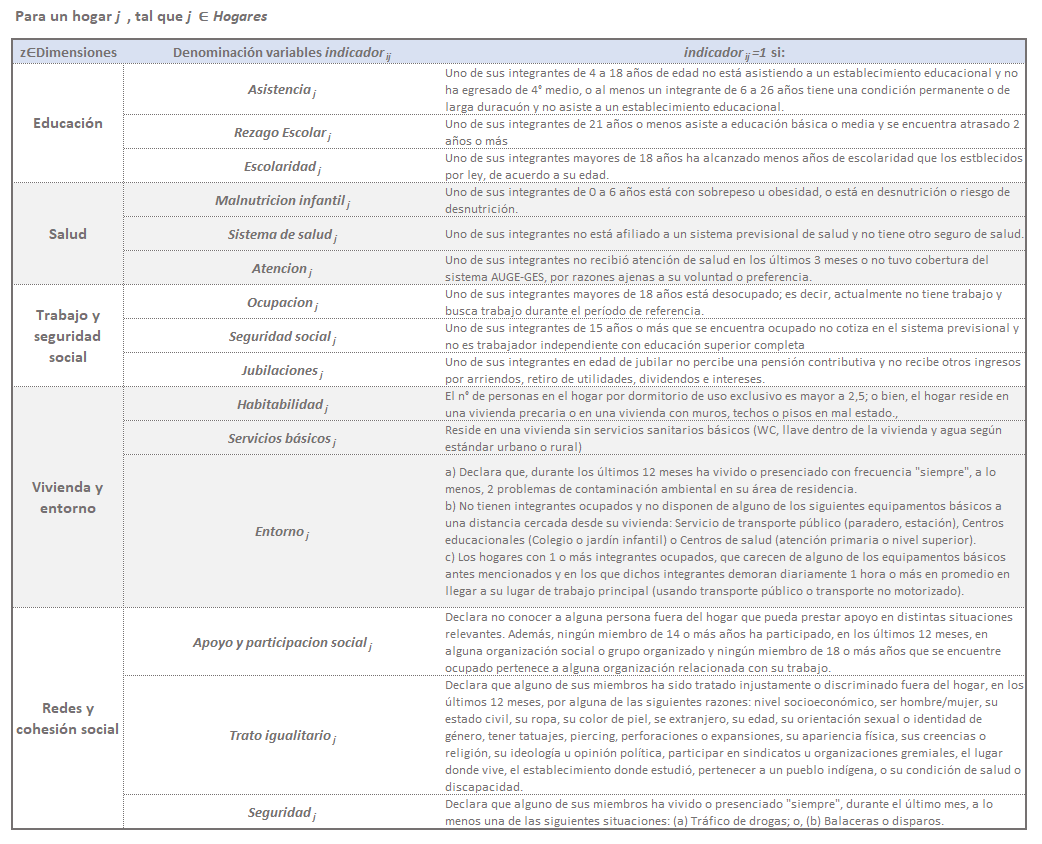
\includegraphics[width=\textwidth]{Max/tabla_indicadores.png}
    \caption{Valorización variables asociadas a carencias. Fuente: elaboración propia.}
    \label{tabla_indicadores}
\end{figure}


\begin{figure}[H]
    \centering
    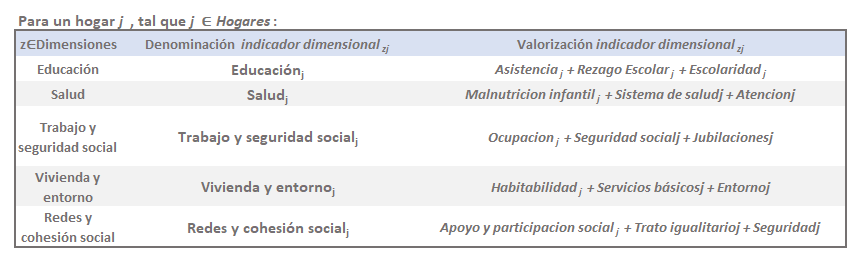
\includegraphics[width=\textwidth]{Max/tabla_indicadores_dimensionales.png}
    \caption{Valorización variables agregadas dimensionales. Fuente: elaboración propia.}
    \label{tabla_indicadores_dimensionales}
\end{figure}
\vspace{2em}


%%%%%%%%%%%%%%%%%%%%%%%%%%%%%%%%%%%%%%%%%%%%%%

\item \textbf{Cálculo de correlaciones entre carencias y dimensiones}

Para cada dupla de indicadores de carencias, se realiza el cálculo del coeficiente phi $\phi$, el cual consiste en una medida de la asociación entre dos o más variables cualitativas. Para este caso en particular, en el que se realiza la comparación de dos variables cualitativas en un dominio de sólo dos categorías (es decir, variables binarias o dicotómicas), el valor del coeficiente phi es equivalente al valor obtenido a través del cálculo del coeficiente de correlación lineal de Pearson \cite{Chedzoy2014Phi-Coefficient}\cite{Chedzoy2006EncyclopediaPhi-coefficient}. El valor del coeficiente phi indicará una mayor intensidad de relación en la medida en que más se acerque en su valor absoluto a 1, y en consecuencia, una menor intensidad de relación en la medida en que el valor se aproxime a 0, asociándose los valores positivos a la co-expresión de ambas variables, y los valores negativos a la co-exclusión.\vspace{1.5em}

Si se consideran como referencias para ejemplificar la obtención del coeficiente phi $\phi$ las carencias $x$ e $y$, se tiene que:
%%%%%%%%%%%%%%%%%%%%%%%%%%%%%%%%%%%%%%%%% carencias x y

\begin{equation}
\begin{split}
indicador_{xj}=\:indicador\:carencia\:x\:del\:hogar\:j\\
indicador_{yj}=\:indicador\:carencia\:y\:del\:hogar\:j
\end{split}
\end{equation}

Luego, para cada hogar pobre multidimensional $j$ se pueden definir las siguientes variables auxiliares:

%%%%%%%%%%%%%%%%%%%%%%%%%%%%%%%%%%%%%%%%% n11 (a)
\begin{equation} \label{n11}
\begin{split}
na_{j}= \begin{cases}
        1;\:si\:indicador_{xj}=\:1\:\ \wedge \:indicador_{yj}=\:1\\
        0;\:e.o.c.
        \end{cases}
\end{split}
\end{equation}
%%%%%%%%%%%%%%%%%%%%%%%%%%%%%%%%%%%%%%%%% n00 (b)
\begin{equation} \label{n00}
\begin{split}
nb_{j}= \begin{cases}
        1;\:si\:indicador_{xj}=\:0\:\ \wedge \:indicador_{yj}=\:0\\
        0;\:e.o.c.
        \end{cases}
\end{split}
\end{equation}
%%%%%%%%%%%%%%%%%%%%%%%%%%%%%%%%%%%%%%%%% n10  (c)
\begin{equation} \label{n10}
\begin{split}
nc_{j}= \begin{cases}
        1;\:si\:indicador_{xj}=\:1\:\ \wedge \:indicador_{yj}=\:0\\
        0;\:e.o.c.
        \end{cases}
\end{split}
\end{equation}
%%%%%%%%%%%%%%%%%%%%%%%%%%%%%%%%%%%%%%%%% n01 (d)
\begin{equation} \label{n01}
\begin{split}
nd_{j}= \begin{cases}
        1;\:si\:indicador_{xj}=\:0\:\ \wedge \:indicador_{yj}=\:1\\
        0;\:e.o.c.
        \end{cases}
\end{split}
\end{equation}


Luego, partir de (\ref{na}), (\ref{nb}), (\ref{nc}) y (\ref{nd}), podemos construir la tabla de contingencia de ambas carencias (fig. \ref{tabla_contingencia}).
%%%%%%%%%%%%%%%%%%%%%%%%%%%%%%%%%%%%%%%%% SUMATORIAS

\begin{equation} \label{na}
\begin{split}
a_{xy}=\sum na_{xy}
\end{split}
\end{equation}

\begin{equation} \label{nb}
\begin{split}
b_{xy}=\sum nb_{xy}
\end{split}
\end{equation}

\begin{equation} \label{nc}
\begin{split}
c_{xy}=\sum nc_{xy}
\end{split}
\end{equation}

\begin{equation} \label{nd}
\begin{split}
d_{xy}=\sum nd_{xy}
\end{split}
\end{equation}\\

%%%%%%%%%%%%%%%%%%

\begin{figure}[H]
    \centering
    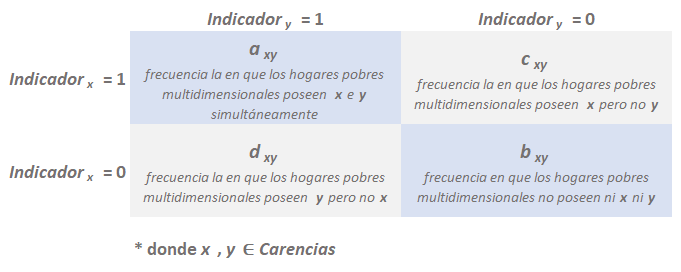
\includegraphics[height=6cm]{Max/tabla_contingencia2.png}
    \caption{Tabla de contingencia carencias $x$ e $y$. Fuente: elaboración propia.}
    \label{tabla_contingencia}
\end{figure}


El coeficiente phi $\phi$ entre las carencias $x$ e $y$ estará dado por:
%%%%%%%%%%%%%%%%%%%%%%%%%%%%%%%%%%%%%%%%  CÁLCULO COEFICIENTE PHI

\begin{equation} \label{calculophi}
\begin{split}
\phi_{xy}=\frac{a_{xy}*b_{xy}-c_{xy}*d_{xy}}{\sqrt{(a_{xy}+c_{xy})(b_{xy}+d_{xy})(b_{xy}+c_{xy})(a_{xy}+d_{xy})}} \: ;\: \phi_{xy} \in [-1;1]
\end{split}
\end{equation}\\

%\( \phi_{xy}=\frac{a*b-c*d}{\sqrt{(a+c)(b+d)(b+c)(a+d)}}\)\vspace{1.5em}\\


Posteriormente, se repite el procedimiento sobre los pares de combinaciones posibles entre las variables dimensionales, empleando como medida de relación el coeficiente de correlación lineal de Pearson $r$. 

Los resultados del cálculo de correlaciones, para ambos conjuntos de variables, se grafican posteriormente en un mapa de calor dispuesto como matriz de doble entrada, en cuyas intersecciones se encuentran representadas numéricamente las correlaciones entre dos indicadores de carencia y entre dos indicadores agregados dimensionales, según corresponda.

\vspace{2em}

\item \textbf{Análisis de red de carencias y red de dimensiones}

Las correlaciones obtenidas en el paso anterior son analizadas mediante el modelo de análisis de red ponderada de correlaciones aplicado al estudio de la pobreza multidimensional, el cual fue propuesto por el sociólogo Pablo Beytía \cite{Beytia2016PobrezaChile}. 

Este modelo supone la construcción de una red no dirigida, para la cual el conjunto de nodos representa al conjunto \textit{Carencias} y el conjunto de arcos representa la relación existente entre los distintos pares de carencias. La intensidad de estas relaciones están caracterizadas mediante el peso de los arcos: si la correlación calculada entre dos carencias $x$ e $y$ (nodos) es mayor o igual a $0$, el peso del arco será igual a $\phi_{xy}$; en caso contrario, si la correlación es menor o igual a $0$, el peso del arco será $0$. De forma gráfica, la diferencia entre el peso de distintos arcos se visualizará en su grosor (fig. \ref{modelo_red_carencias}).


%el que corresponde al coeficiente $\phi$ entre las carencias que vincula (de forma gráfica, el peso se visualizará mediante el grosor del arco). De manera formal, dado un conjunto de nodos \textit{N}, donde \textit{N}=\textit{Carencias}, se define \textit{S} como el conjunto de 2-combinaciones de los elementos del conjunto \textit{N} que representa el conjunto de arcos no dirigidos, caracterizados por el coeficiente phi entre las carencias representadas por nodos enlazados (fig. \ref{modelo_red_carencias}).

\begin{figure}[H]
    \centering
    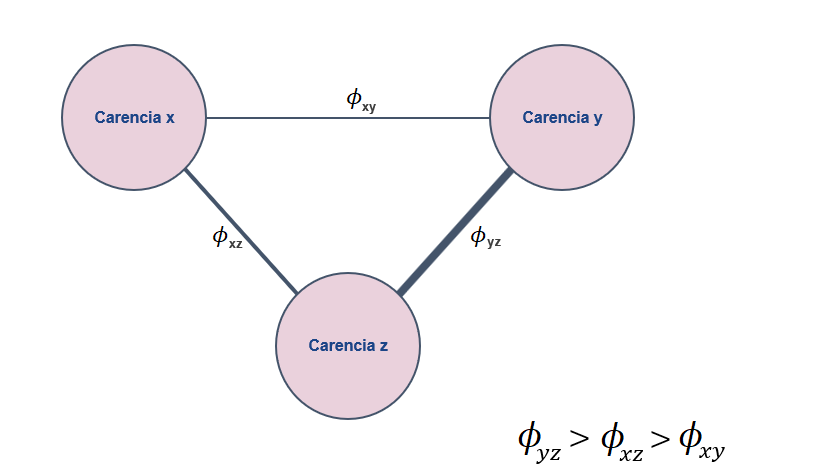
\includegraphics[height=6cm]{Max/redes_phi.png}
    \caption{Modelo red de carencias. Fuente: elaboración propia, basada en modelo de Beytía \cite{Beytia2016PobrezaChile}.}
    \label{modelo_red_carencias}
\end{figure}

Este procedimiento se realiza nuevamente, esta vez representando en los nodos al conjunto \textit{Dimensiones}, en los arcos a las variables agregadas dimensionales, y el pesos de los arcos los valores positivos obtenidos para el cálculo del coeficiente de Pearson entre las variables agregadas dimensionales (fig. \ref{modelo_red_dimensiones}).


\begin{figure}[H]
    \centering
    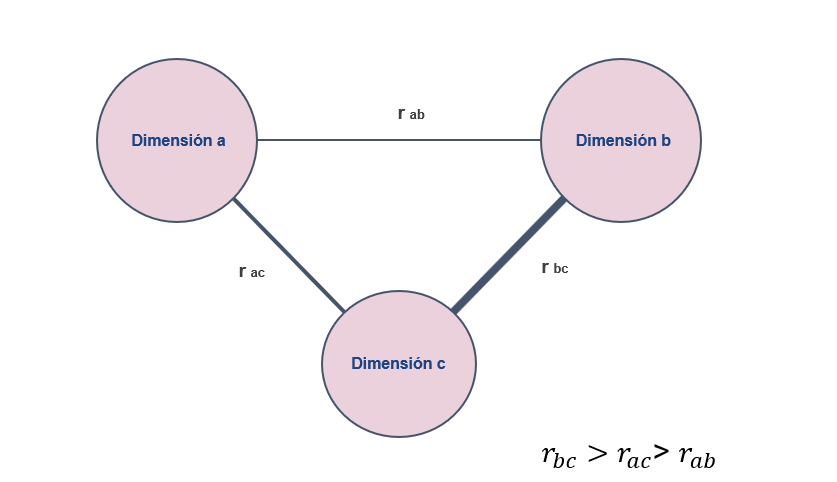
\includegraphics[height=6cm]{Max/redes_pearson.png}
    \caption{Modelo red de dimensiones. Fuente: elaboración propia, basada en modelo de Beytía \cite{Beytia2016PobrezaChile}.}
    \label{modelo_red_dimensiones}
\end{figure}

Posteriormente, y mediante el empleo de la herramienta de análisis de redes \textit{Gephi} se realizará el cálculo de las centralidades de las carencias (grados nodales) y del grado de intermediación, que nos indica el peso estructural de las carencias y el grado en que una carencia actúa de enlace entre otras dos carencias que no se encuentran vinculadas directamente entre sí, respectivamente. 

\end{enumerate}


\subsection{Metodología análisis relacional de la pobreza multidimensional por tipo de hogar y tipologías}

La metodología descrita en esta etapa constituye, en primera instancia, una continuación de la ya descrita, esta vez ajustando el enfoque del análisis relacional mediante la división de la muestra de hogares pobres multidimensionales según su clasificación. Posteriormente, la metodología se centra en el análisis de las distintas conformaciones de carencias que caracterizan a los hogares pobres multidimensionales, así como de 2 factores externos al \textit{IPM} que pueden afectar su prevalencia (zona de residencia y número de personas que componen el hogar). Finalmente, se describirá la metodología del análisis comparativo entre el nivel de ingreso de los hogares pobres multidimensionales  y el nivel de pobreza multidimensional, expresada en el \textit{IPM}. 



\subsubsection{Metodología análisis relacional por tipo de hogar}
    

\begin{enumerate}

\item \textbf{Clasificación de hogares}

La clasificación de los hogares se basa en la distinción empleada por el Ministerio de Desarrollo Social y Familia, la cual establece 6 categorías: \textit{Unipersonal}, \textit{Nuclear Monoparental}, \textit{Nuclear Biparental}, \textit{Extendido Monoparental}, \textit{Extendido Biparental} y \textit{Censal}. Con el fin de identificar los criterios de clasificación para cada tipo, es necesario considerar las siguientes definiciones:
\begin{itemize}
    \item \textbf{Hogar:} ``se consideran miembros de un hogar a todas aquellas personas que, siendo residentes de una misma vivienda, pueden tener o no vínculos de parentesco entre sí y habitualmente hacen vida en común, es decir, se alojan y se alimentan juntas. Dicho de otra forma, habitan en la misma vivienda y tienen presupuesto de alimentación común. Un hogar puede estar constituido por una persona o un grupo de personas. Puede ocurrir que en una vivienda exista uno o más hogares. Sin embargo, un hogar no puede ocupar más de una vivienda.
Se excluyen aquellas personas que estuvieron ausentes más de seis meses en el último año, exceptuándose el jefe del hogar y los niños menores de seis meses''. \cite{MDS2019Manual2017}
    
    \item \textbf{Jefe(a) de hogar:} ``es aquel miembro (hombre o mujer) considerado como tal por las otras personas del hogar, ya sea por razones de dependencia económica, parentesco, edad, autoridad o respeto. En todos los hogares se identifica un solo jefe o jefa''. \cite{MDS2019Manual2017}
    
    \item \textbf{Núcleo familiar:} ``es una parte de un hogar (es decir, un subconjunto de sus miembros) y puede estar constituido por una persona sola o un grupo de personas. Comúnmente corresponden a parejas o adultos/as junto a una o más personas que dependen de ellos/as. Puede ocurrir que en un hogar exista uno o más núcleos familiares. Sin embargo, no puede darse que un núcleo familiar esté distribuido en más de un hogar''. \cite{MDS2019Manual2017}
\end{itemize}

En otras palabras, un hogar se define como el conjunto de personas que habitan en la misma vivienda y comparten gastos de alimentación. Al no mediar necesariamente relaciones familiares en su conformación. se define un núcleo familiar como el subconjunto de miembros de un hogar que comparten un tipo de relación más estrecha, en general de parentesco. Bajo esta definición, una vivienda puede albergar a más de un hogar, y un hogar a su vez puede estar constituido por uno o más núcleos. Por el contrario, un núcleo no puede pertenecer a más de un hogar, y un hogar no puede pertenecer a más de una vivienda.


Los tipos de hogares se definen en función de los núcleos familiares que los componen y de las relaciones existentes entre el o la designada como Jefe(a) de hogar y el resto de los miembros del hogar, según los siguientes criterios\footnote{Los criterios de clasificación utilizados para la distinción de los tipos de hogares se basan en la información obtenida de forma directa en la Secretaría Regional Ministerial de Desarrollo Social y Familia Metropolitana del Gobierno de Chile.}:

\begin{itemize}
    \item \textbf{Unipersonal:} hogares conformados por solo un integrante.
    
    \item \textbf{Nuclear Monoparental:} hogares conformados por dos o más personas pertenecientes a un mismo núcleo, y cuyo Jefe(a) de hogar no tiene una relación de pareja (formal o informal) con otro miembro del hogar (de distinto o igual sexo).
    
    \item \textbf{Nuclear Biparental:} hogares conformados por dos o más personas pertenecientes a un mismo núcleo, y cuyo Jefe(a) de hogar tiene una relación de pareja (formal o informal) con otro miembro del hogar (de distinto o igual sexo).
    
    \item \textbf{Extendido Monoparental:} hogares conformados por más de un núcleo (donde al menos uno está conformado por dos o más miembros), y cuyo Jefe(a) de hogar no tiene una relación de pareja (formal o informal) con otro miembro del hogar (de distinto o igual sexo).
    
    \item \textbf{Extendido Biparental:} hogares conformados por más de un núcleo (donde al menos uno está conformado por dos o más miembros), y cuyo Jefe(a) de hogar tiene una relación de pareja (formal o informal) con otro miembro del hogar (de distinto o igual sexo).
    
    \item \textbf{Censal:} hogares conformados por dos o más personas sin relaciones familiares (cada persona constituye un núcleo familiar diferente).
\end{itemize}

A continuación ilustrará el criterio de clasificación mediante un ejemplo sencillo:

\begin{itemize}
    \item En una casa (\textit{vivienda}) residen 2 estudiantes universitarios: Magdalena y Domingo. Debido a que no comparten un presupuesto de alimentación (i.e. realizan las compras de víveres por separado),  cada uno de ellos constituye un hogar independiente. Al ser cada uno de ellos los únicos miembros de sus hogares respectivos, ambos hogares serían del tipo \textbf{unipersonal}.
    
    \item Eventualmente, los estudiantes deciden empezar a compartir los gastos de alimentación para aprovechar los beneficios de unir ambos presupuestos.  Desde ese momento pasan a constituir un único hogar. Sin embargo, debido a que la relación que los vincula se basa solo en un motivo económico (y no de dependencia o parentesco), cada uno de ellos constituye un núcleo familiar independiente. Luego, al estar el hogar conformado por 2 personas, cada una de las cuales constituye un núcleo diferente, este se clasificaría como \textbf{censal}.
    
    \item Con el tiempo ambos estudiantes estrechan su relación, inician una relación de pareja y tienen un hijo. Ahora se puede decir que, al existir un vínculo de familiaridad y dependencia entre ellos (y su hijo), los tres conforman un solo núcleo familiar, y un sólo hogar. Magdalena es quien, en general, toma las decisiones del hogar, por lo que se le puede identificar como \textit{jefa de hogar}. Al tener Magdalena una pareja dentro del hogar (Domingo), y debido a que los tres miembros del hogar conforman un solo núcleo, el hogar se clasificaría como \textbf{nuclear biparental}.
    
    \item Luego de un par de años, Magdalena y Domingo deciden terminar su relación, por lo que Domingo se traslada a otra residencia (deja, por lo tanto, de pertenecer al hogar y al núcleo familiar). Magdalena y su hijo aún conforman un hogar y un núcleo. Ahora bien, debido a que ella, como jefa de hogar no tiene una relación de pareja con otro miembro del hogar, junto a su hijo conforman un hogar clasificado como \textbf{nuclear monoparental}. 
    
    \item Con el fin de mejorar su economía familiar, Magdalena comienza a arrendarle una habitación de huéspedes a sus amiga Inés y Sonja, y juntas deciden además compartir gastos de alimentación (por lo tanto conforman, junto al hijo de Magdalena, un sólo hogar). Al no mediar una relación de parentesco o dependencia entre ellas, Inés y Sonja constituyen, cada una de ellas, un núcleo familiar independiente, y debido a que Magdalena (jefa de hogar) no tiene una relación de pareja con otro miembro del hogar, el hogar que constituyen es del tipo \textbf{extendido monoparental}.
    
    \item Finalmente, Magdalena estrecha su relación con Sonja y comienzan una relación de pareja. Sonja desde entonces pasa a constituir parte del núcleo familiar de Magdalena. El hogar entonces queda constituido por dos núcleos: el de Magdalena, su hijo y Sonja, y el de Inés. Al tener Magdalena (jefa de hogar) una pareja dentro del hogar, los cuatro conforman un hogar \textbf{extendido biparental}.
    
\end{itemize}

\vspace{2em}


\item \textbf{Análisis de red de carencias por tipo de hogar}

Para cada subconjunto de la muestra particionada según la clasificación por tipo de hogar definida en el punto anterior, se efectuará el cálculo del coeficiente $\phi$ entre cada dupla de carencias y, posteriormente, el análisis de red de carencias, siguiendo el mismo procedimiento empleado anteriormente para el conjunto total de hogares pobres multidimensionales.

\end{enumerate}


%%%%%%%%%%%%%%%%%%%%%%%%%%%%%%%%%%%%%%%%%%%%%%%%%%%%%%%%%%%%%%%%%%%%%%%%%%%%%%


\subsubsection{Metodología análisis tipológico}


\begin{enumerate}
\item \textbf{Cálculo del \textit{IPM} por hogar}

Para cada hogar clasificado como pobre multidimensionalmente se calculará el \textit{IPM}\footnote{Si bien la base de datos de la encuesta CASEN 2017 dispuesta por el Ministerio de Desarrollo Social y Familia incluye la clasificación de cada hogar en \textit{pobre} y \textit{no pobre} respecto a la pobreza multidimensional, no incorpora el valor calculado para el \textit{IPM}}, según la ponderación del modelo de 5 dimensiones (fig. \ref{ponderaciones}).

\begin{figure}[H]
    \centering
    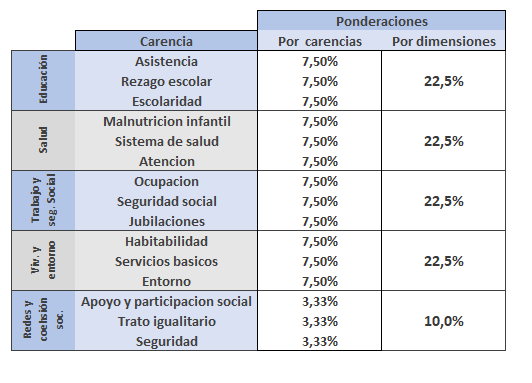
\includegraphics[height=9cm]{Max/ponderaciones.png}
    \caption{Ponderaciones de carencias y dimensiones para el cálculo del \textit{IPM} - CASEN 2017. Fuente: elaboración propia.}
    \label{ponderaciones}
\end{figure}

\vspace{2em}

\item \textbf{Determinación tipologías}


 Se calculará la frecuencia del conjunto de combinaciones posibles entre las 15 carencias del modelo de pobreza multidimensional de 5 dimensiones, para los hogares pobres multidimensionales registrados en la encuesta CASEN 2017. Cada una de estas combinaciones configura una tipología específica de la estructura de carencias, la cual será caracterizada por un \textit{IPM} asociado.
 
 \vspace{2em}

\item \textbf{Determinación tipologías por factores externos}

El procedimiento de determinación de tipologías y análisis de frecuencia se realizará nuevamente, esta vez  aplicando el principio de descomponibilidad a través de una partición los datos según los siguientes factores externos:

    \begin{itemize}
        \item  \textbf{Zona} (de residencia), pudiendo los hogares pertenecer a las categorías \textit{rural} y \textit{urbano}. 
        \item \textbf{Número de integrantes} que conforman el hogar, sin considerar al personal de servicio doméstico puertas adentro. 
    \end{itemize}
\end{enumerate}


\subsubsection{Metodología análisis comparativo con nivel de ingresos}

La metodología descrita a continuación busca comprender la relación entre los niveles de ingresos de los hogares pobres multidimensionales y sus estructuras de carencias, empleando como medida de referencia la línea de la pobreza por ingresos (\textit{LP}). 

La línea de la pobreza es definida por la \textit{CEPAL} como la representación de un valor monetario en el que se considera el costo de adquisición de una canasta básica de alimentos (\textit{CBA})\footnote{La \textit{CBA} se construye, según la \textit{CEPAL},  ``de manera que satisfaga los requerimientos calóricos promedio de la población, mediante una estructura de bienes y precios proveniente de las pautas de consumo observadas en un grupo de referencia y ajustada de manera que cuente con equilibrios nutricionales básicos''\cite{CEPAL2018MedicionResultados}.}, expresado sobre la base de la relación entre el gasto total y el gasto en alimentos \cite{CEPAL2018MedicionResultados}. La medición de la pobreza por ingresos, se determina mediante la comparación entre el ingreso percibido del hogar y el ingreso mínimo necesario para satisfacer las necesidades básicas que están representadas en la \textit{CBA}, siendo el valor de \textit{LP} el ingreso necesario para financiar la \textit{CBA}. La línea de la pobreza es calculada regularmente por el Ministerio de Desarrollo Social y Familia, y en su determinación se realiza además un ajuste en función del número de personas que integran el hogar, debido a que se supone la existencia de economías de escala para ciertos gastos. En consecuencia, todos aquellos hogares cuyos niveles de ingresos sean inferiores a \textit{LP}, serán catalogados como pobres por ingresos \cite{CEPAL2018Medicion2017}.


Ante la inexistencia de una metodología oficial del Gobierno de Chile que defina una estratificación socio-económica, el centro de estudios e investigación privado \textit{Libertad y Desarrollo} realizó el año 2019 una propuesta de clasificación socio-económica expresada en términos del nivel de ingresos relativo a la línea de la pobreza, con el fin de acercarse al marco metodológico empleado por el Banco Mundial \cite{LibertadyDesarrollo2019HaciaChile}. Esta propuesta considera 6 categorías socio-económicas, definidas como se indica en la fig. \ref{clasld}.


\begin{figure}[H]
    \centering
    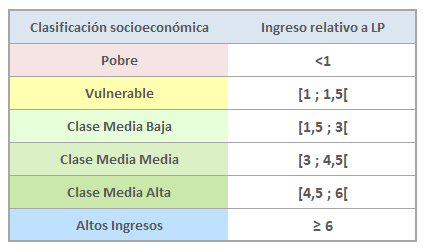
\includegraphics[height=6cm]{Max/clasificacion_ld.png}
    \caption{Propuesta \textit{Libertad y Desarrollo} de clasificación socio-económica por ingreso, expresado en términos de \textit{LP}. Fuente: elaboración propia, a partir de información dispuesta por \textit{Libertad y Desarrollo} \cite{LibertadyDesarrollo2019HaciaChile}. }
    \label{clasld}
\end{figure}



\begin{enumerate}
    


\item \textbf{Definición variable relativa de ingreso}

Para simplificar el análisis respecto al ingreso de los hogares, este se realizará empleando el indicador relativo del ingreso ajustado del hogar respecto a la línea de la pobreza. Para cada hogar $j$, el indicador relativo $ingreso\:relativo_{j}$ se define como el cociente entre el producto del ingreso \textit{per cápita} del hogar corregido (\textit{ypc}) y el número de personas de componen el hogar $n_{j}$,  y la línea de pobreza (\textit{LP}) ajustada según el número de personas que componen el hogar $LP_n$. Se emplearán como referencia para la \textit{LP} los valores calculados por el Ministerio de Desarrollo Social y Familia en el mes de noviembre de 2017 (fig. \ref{LPLPE}).

\begin{equation} \label{calculophi}
\begin{split}
ingreso\:relativo_{j}=\frac{ypc_{j}*n_{j}}{LP_{n}}\: ;\:n=n_{j}
\end{split}
\end{equation}\\

%\( \phi_{xy}=\frac{a*b-c*d}{\sqrt{(a+c)(b+d)(b+c)(a+d)}}\)\vspace{1.5em}\\



\begin{figure}[H]
    \centering
    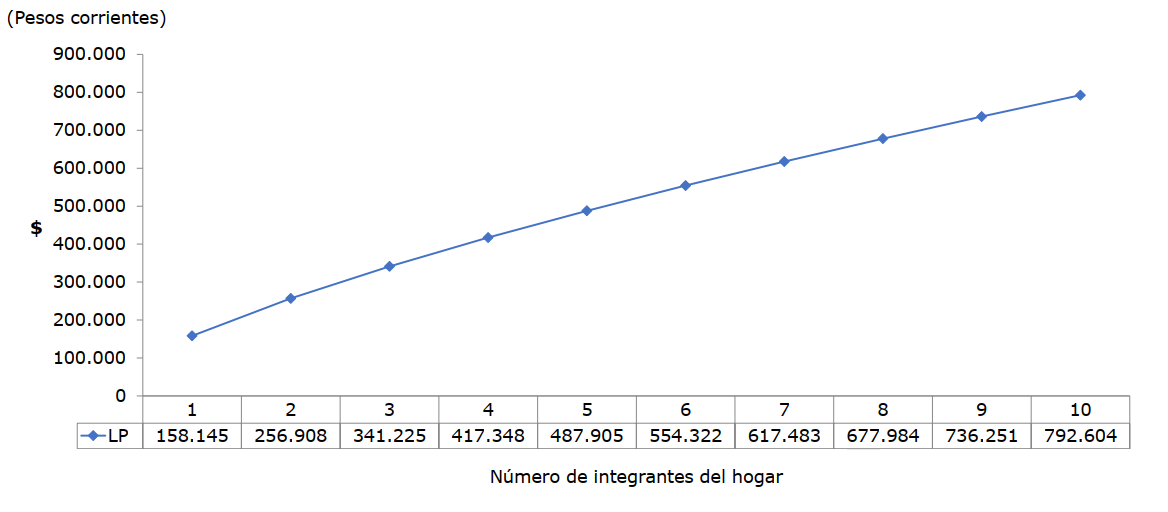
\includegraphics[width=\textwidth]{Max/linea_pobreza.png}
    \caption{Valor de la línea de la pobreza ($LP_n$) en función del número de integrantes del hogar $n$, Noviembre 2017. Fuente: Ministerio de Desarrollo Social y Familia}
    \label{LPLPE}
\end{figure}

\vspace{2em}

\item \textbf{Clasificación hogares pobres multidimensionales por estrato socio-económico}

Los hogares pobres multidimensionales se clasificarán en distintos intervalos socio-económicos, según el criterio propuesto por \textit{Libertad y Desarrollo}, con el objetivo de identificar el grado de contribución de cada categoría al total de hogares pobres multidimensionales.

\vspace{2em}


\item \textbf{Comparación indicador ingreso relativo e \textit{IPM}}
Los valores obtenidos para el indicador relativo de ingreso de cada hogar pobre dimensional se grafican en función del índice de pobreza multidimensional, a través de un diagrama de dispersión. El grado de relación entre ambas variables se medirá empleando para ello el coeficiente de correlación lineal de Pearson. 

\vspace{2em}


\item \textbf{Comparación indicador ingreso relativo y padecimiento de carencias}

Con el fin de determinar la relación particular entre el padecimiento de una carencia del modelo de 5 dimensiones y el nivel de ingreso de los hogares, se analizará la distribución del indicador relativo de ingreso para cada conjunto de hogares pobres multidimensionales que padezcan una carencia en particular. 

\end{enumerate}




\newpage
\subsection{Metodología análisis de sensibilidad del \textit{IPM} y proyecciones de la pobreza multidimensional}


\subsubsection{Metodología análisis de sensibilidad del \textit{IPM}}


Se recalculará el índice de pobreza multidimensional de los hogares de la muestra CASEN 2017, esta vez ponderando cada indicador de carencias de igual forma (fig. \ref{ponddos}). 

\begin{figure}[H]
    \centering
    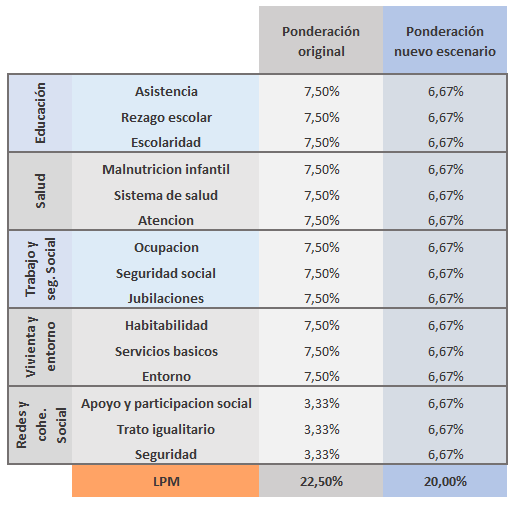
\includegraphics[height=10cm]{Max/ponderaciones_sensib.png}
    \caption{Ponderación de carencias para análisis de sensibilidad del \textit{IPM}. Fuente: elaboración propia.}
    \label{ponddos}
\end{figure}

La línea de la pobreza multidimensional (\textit{LPM}) empleada originalmente, se determinó en función de la ponderación del \textit{IPM} en hogares que padecen un mínimo de tres carencias pertenecientes a las dimensiones \textit{Educación}, \textit{Salud}, \textit{Vivienda y entorno} y \textit{Trabajo y seguridad social}, correspondiente a un 22.5\%. En lineamiento con lo anterior, la línea de pobreza dimensional definida para el nuevo escenario, corresponderá a la ponderación del \textit{IPM} de los hogares que padecen un mínimo de tres carencias, siendo estas pertenecientes a cualquiera de las cinco dimensiones (es decir, incluyendo la dimensión \textit{Redes y cohesión social}), correspondiente a un 20\%. 

Habiendo obtenido una nueva distribución de la pobreza multidimensional, se realizará nuevamente un análisis reticular de las carencias de los hogares pobres multidimensionales.




\subsubsection{Metodología proyecciones de la pobreza multidimensional}
Se realizará una proyección del \textit{IPM} promedio y de la prevalencia de la pobreza multidimensional para el segundo semestre de 2020. Esta se construirá en base a la proyección de la incidencia las carencias \textit{Ocupación} y \textit{Seguridad}, bajo el supuesto \textit{ceteris paribus} respecto a la medición del resto de carencias en la encuesta CASEN 2017. En otras palabras, se trabajará bajo el supuesto de que para ninguna de las carencias contempladas en el modelo trabajado (exceptuando \textit{Ocupación} y \textit{Seguridad}), han existido variaciones significativas en los últimos tres años. 

\begin{enumerate}

    \item \textbf{Proyección prevalencia Ocupación}
    
    Para la proyección de la frecuencia de la carencia \textit{ocupación} en los hogares, se asumirá la existencia de una relación directamente proporcional entre la tasa de desocupación estimada por el \textit{INE}\footnote{El Instituto Nacional de Estadísticas emite periódicamente boletines con la estimación de la tasa desocupación, los cuales están disponibles en el sitio \url{https://www.ine.cl/estadisticas/sociales/mercado-laboral/ocupacion-y-desocupacion}}. Si definimos $f.carencia ocupacion$ como la frecuencia porcentual de hogares que padecen la carencia de \textit{ocupación}, $t. desocupacion$ como la tasa de desocupación estimada por el \textit{INE}, $t$ como el período de referencia para el cálculo, y $t+h$ como el período sobre el cual se realiza la proyección, la proyección de la frecuencia de la carencia \textit{ocupación}, en el período $t+h$ estará dada por:
    
    \begin{equation}\label{calculo_proyeccion_ocupacion}
        \begin{split}
            f.carencia\:ocupacion_{t+h}=\frac{t.desocupacion_{t+h}*f.carencia\:ocupacion_t}{t.desocupacion_t}\\
        \end{split}
    \end{equation}
    
    \vspace{2em}
    
    
    
    
    \item \textbf{Proyección prevalencia Seguridad}
    
    La proyección de la carencia \textit{seguridad} se realizará de forma similar a la de \textit{ocupación}, pero empleando como medida referencial el índice de \textit{percepción del aumento de la delincuencia y exposición frente al delito} \footnote{El Instituto Nacional de Estadísticas emite anualmente un boletín con los resultados de la Encuesta Nacional Urbana de Seguridad Ciudadana (ENUSC), la cual incorpora el indicador de \textit{Percepción del aumento de la delincuencia y exposición frente al delito}. Los resultados de la ENUSC se encuentran disponibles en el sitio \url{https://www.ine.cl/estadisticas/sociales/seguridad-publica-y-justicia/seguridad-ciudadana}}. De esta forma, si definimos $f.carencia seguridad$ como la frecuencia porcentual de hogares que padecen la carencia de \textit{seguridad}, $i. seguridad$ como la estimación de la percepción del aumento de la delincuencia y exposición frente al delito realizada por el \textit{INE}, $t$ como el período de referencia para el cálculo, y $t+h$ como el período sobre el cual se realiza la proyección, la proyección de la frecuencia de la carencia \textit{seguridad}, en el período $t+h$ estará dada por \ref{calculo_proyeccion_seguridad}.
    
    \begin{equation}\label{calculo_proyeccion_seguridad}
        \begin{split}
            f.carencia\:seguridad_{t+h}=\frac{i.seguridad_{t+h}*f.carencia\:seguridad_t}{i.seguridad_t}\\
        \end{split}
    \end{equation}
    
    
    \item \textbf{Proyección IPM}


Para la proyección del \textit{IPM} en el período $t+h$ se empleará el método \textit{Montecarlo}. Este corresponde a una metodología de simulación empleada para la estimación de variables no determinísticas, cuando su cálculo de forma analítica es demasiado complejo. El método \textit{Montecarlo}, para este caso en particular, se puede definir a través de los siguientes pasos:

\vspace{2em}

\underline{Paso 1 - Definición de las medidas de desempeño:} 

El método se aplicará para estudiar, como se mencionó, variables no determinísticas complejas, que corresponderán a las medidas de desempeño. En el caso particular del presente estudio, estas medidas de desempeño corresponderán a 1- \textit{IPM} promedio de hogares; 2- Desviación estándar del \textit{IPM} de los hogares; y 3- Frecuencia porcentual de los hogares pobres multidimensionales.

\vspace{2em}
        
\underline{Paso 2- Definición de un modelo de entrada:} 

Se definen los parámetros y la distribución de las variables aleatorias sobre los que se realiza el cálculo de las medidas de desempeño. Para este caso en particular, los parámetros corresponderán al conjunto de valores de los indicadores de cada carencia (con excepción de las carencias ocupación y seguridad), así como las ponderaciones empleadas para el cálculo del \textit{IPM}. Las variables aleatorias del modelo de entrada corresponderán a los indicadores por hogar de las carencias \textit{ocupación} y \textit{seguridad}, para las cuales se asumirá una distribución \textit{Bernoulli}\footnote{Este supuesto se empleará para simplificar el cálculo de la proyección del \textit{IPM}. En la realidad pueden existir diferencias en la distribución de ambas carencias para distintos grupos demográficos (determinados por factores como la zona y región de residencia, el rubro en el que se desempeñan las personas y el nivel de escolaridad, entre muchos otros.} con un valor $p$ estimado a partir de las frecuencias proyectadas de cada carencia.\\
        

        Dado el conjunto $Hogares$, donde $j \in Hogares$, se definen los parámetros $Asistencia_j$, $Escolaridad_j$, $Rezago\:escolar_j$, $Malnutricion \:infantil_j$, $Atencion_j$, $Sistema \: de \:salud_j$, $Seguridad\:social_j$, $Jubilaciones_j$, $habitabilidad_j$, $servicios\:basicos_j$, $entorno_j$; $trato\:igualitario_j$ y $apoyo\:y\:participacion\:social_j$ como los indicadores asociados a las carencias, para todos los hogares $j\in Hogares$.\\ 
        
        Se definen las variables aleatorias $ocupacion_j$ y $seguridad_j$, como los valores de los indicadores de las carencias \textit{ocupación} y \textit{seguridad}, para todo $h\in Hogares$.
        
        
        \begin{equation} \label{bernoulli}
        \begin{split}
        ocupacion_j\sim Be(p)\\
        seguridad_j\sim Be(q)
        \end{split}
        \end{equation}
        
        \begin{equation} \label{bernoulli}
        \begin{split}
        p=  f.carencia\:ocupacion_{t+h}\\
        q=  f.carencia\:seguridad_{t+h}
        \end{split}
        \end{equation}


\vspace{2em}        

\underline{Paso 3 - Generación de datos aleatorios:} 

Se generará un conjunto de valores aleatorios para las variables asociadas a las carencias ocupación y seguridad definidas en el paso anterior, empleando la distribución estimada para cada una de ellas. 


\vspace{2em}

\underline{Paso 4 - Obtención medidas de desempeño:} 

Se realizará el cálculo de las medidas de desempeño definidas en el paso 1, empleando para ello los parámetros definidos en el paso 2 y los valores de las variables aleatorias obtenidas en 3. 


\vspace{2em}

\underline{Paso 5- Estimación de medidas de desempeño:} 

Los pasos 3 y 4 se iterarán, almacenando en cada ciclo los valores obtenidos en el cálculo de las medidas de desempeño. Se realizará la estimación de las medidas de desempeño, empleando como estimador el promedio de las observaciones realizadas en cada iteración. El número de iteraciones (largo de la simulación) se ampliará hasta que se observe que el promedio de las observaciones de las medidas de desempeño converja en un valor definido. 

   
 
    
    
   

    
    
    
    

    
    
\end{enumerate}













\newpage
\section{Resultados obtenidos} % 30 puntos




\subsection{Resultados PARTE I}
\begin{enumerate}
\item \textbf{Obtención de variables} \\
 La encuesta CASEN 2017 recoge una muestra de 216.439 personas, agrupadas en un total de 70.948 hogares. De ellas, 206.572 personas (95\% del total), pertenecientes a su vez a 67.820 hogares, cuentan con todos los indicadores de carencias requeridos. De este universo, un total de 44.972 personas (21\% ), pertenecientes a su vez a 12.392 hogares, son catalogadas como pobres según el criterio multidimensional de 5 dimensiones. Las variables de entrada del modelo corresponden a los indicadores de carencias para cada hogar (12.392 indicadores de carencia por cada una de las 15 carencias), y los indicadores agregados dimensionales (12.392 indicadores dimensionales por cada una de las 5 dimensiones).
 
 En la Figura \ref{pobresXpersona} y en la Figura \ref{pobresXhogar} se muestran las distribuciones de la pobreza multidimensional por personas y por hogares respectivamente.  

\begin{figure}[H]
    \centering
    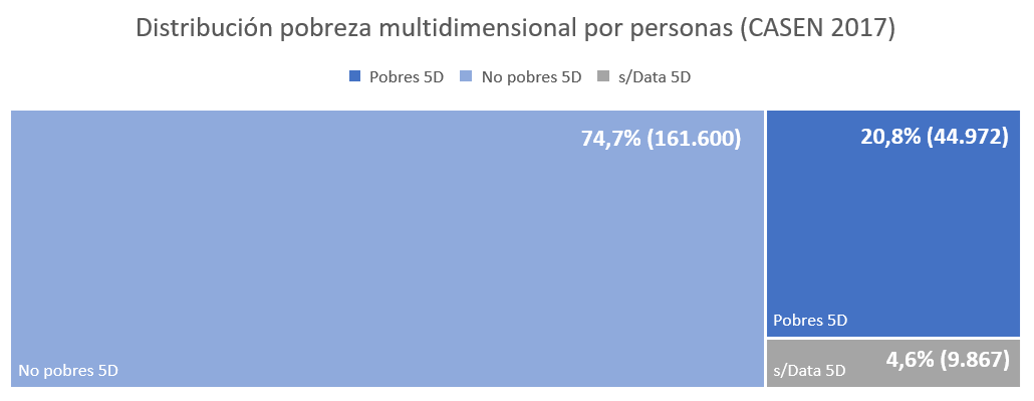
\includegraphics[width=\textwidth]{Mati N/pobrezaXpersonas.png}
    \caption{Distribución pobreza multidimensional por personas CASEN 2017. Fuente: Elaboración propia.}
    \label{pobresXpersona}
\end{figure}

\begin{figure}[H]
    \centering
    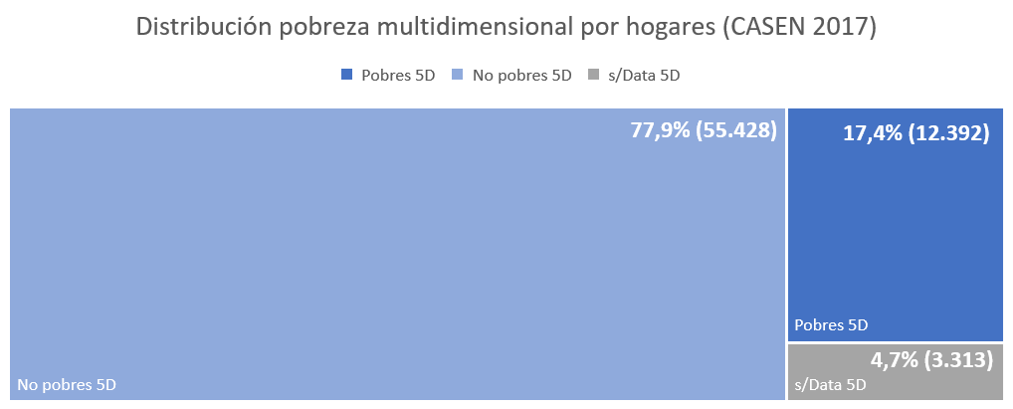
\includegraphics[width=\textwidth]{Mati N/pobrezaXhogares.png}
    \caption{Distribución por tipo de hogares CASEN 2017. Fuente: Elaboración propia.}
    \label{pobresXhogar}
\end{figure}
 
 \item \textbf{Cálculo de correlaciones entre carencias y dimensiones}\\
 Para el cálculo y graficación de los coeficientes de Pearson, tanto para las carencias como para las dimensiones, así como de los coeficientes de determinación para cada combinación de dimensiones, se emplearon las bibliotecas de software libre NumPy y Pandas (Python).
 
 Habiéndose calculado los coeficientes de correlación entre las distintas carencias, detallado en la Figura \ref{pearsoncarencias}, se obtuvieron, sobre un total de 105 combinaciones, 70 valores negativos (67\%) y 35 valores positivos (33\%), comprendidos en el intervalo [0,0018;0,0968], por lo que se podría inferir una relación nula o insignificante. Por el contrario, se puede observar que existe un grado de significancia débil negativa, dentro del intervalo [-0,3670;-0,1925], para dos correlaciones (Entorno v/s Seguridad social y Habitabilidad v/s Jubilaciones). 
%%%%%%%%%%%%%%%%%%%% índice de pearson carencias
\begin{figure}[H]
    \centering
        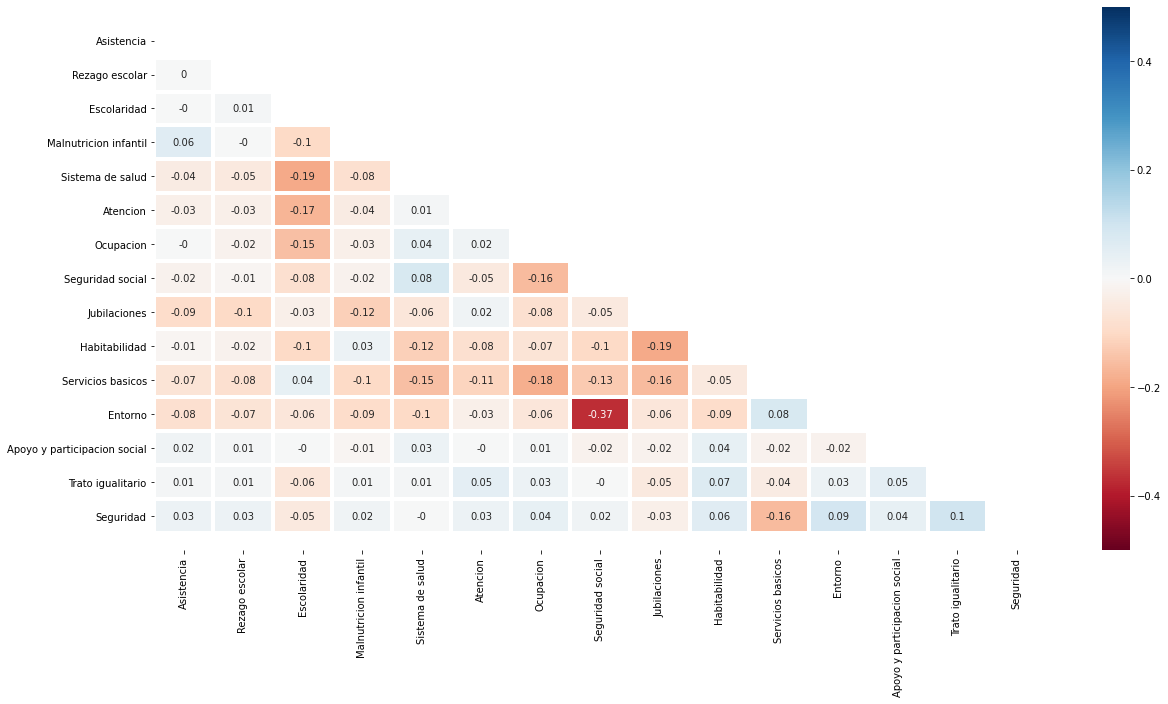
\includegraphics[width=\linewidth]{Heatmaps/Heatmap_pearson_Correlaciones.png}
    \caption{Mapa de calor coeficiente correlación de Pearson por carencias. Elaboración propia.}
    \label{pearsoncarencias}
\end{figure}

Los resultados del análisis de correlación para variables definidas por dimensión, presentado en la Figura \ref{PearsonDim}, muestran para un total de 10 combinaciones, sólo 2 relaciones positivas de significancia nula o insignificantes en el intervalo [0,0187;0,0435]. Por el contrario, de las 8 combinaciones restantes, 2 indican significancia débil negativa dentro del intervalo [-0,2684;-0,2324] (Salud v/s Educación y Salud v/s Vivienda y entorno), y una presenta una significancia fuerte negativa de -0,5076 (Vivienda y entorno v/s Trabajo y seguridad social).

%%%%%%%%%%%%%%%%%%%% índice de pearson DIM
\begin{figure}[H]
    \centering
        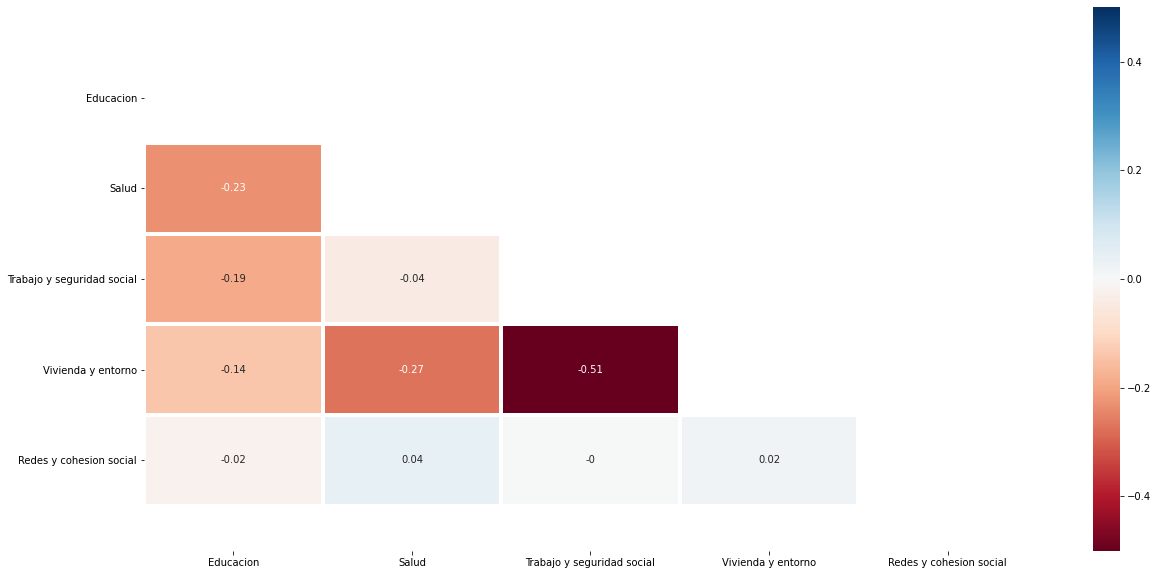
\includegraphics[width=\linewidth]{Heatmaps/Heatmap_pearson_DIM.png}
    \caption{Mapa de calor coeficiente correlación de Pearson por dimensiones. Elaboración propia}
    \label{PearsonDim}
\end{figure}

\item \textbf{Análisis de red de carencias y red de dimensiones}\\
Habiéndose obtenido valores de correlaciones positivos y negativos, se presentan ambos conjuntos en grafos separados (Figura \ref{grafoPos} y Figura \ref{grafoNeg}), incluyéndose en la representación de los grafos de las correlaciones entre dimensiones, los respectivos coeficientes de determinación r-cuadrado (Fig. \ref{grafodimpos} y \ref{grafodimneg}). Se puede apreciar que los valores de r-cuadrado, indican en general bajos niveles de fiabilidad para el modelo (menores a un 10\% de ajuste), con la excepción de la correlación entre las dimensiones de Trabajo y seguridad social, y Vivienda y entorno (25,76\%).
%%%%%%%%%%%%%%%%%%%% grafo carencias positivas
\newpage
\begin{figure}[H]
    \centering
        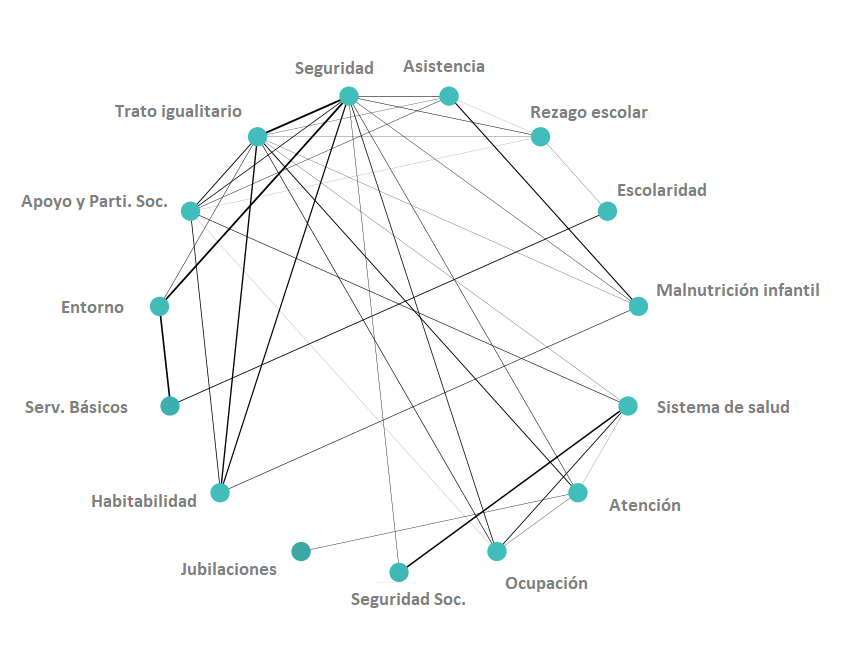
\includegraphics[width=11cm]{Grafos/GrafoCarencias.png}
    \caption{Red de carencias con coeficientes de correlación positivos. Elaboración propia}
    \label{grafoPos}
\end{figure}
%%%%%%%%%%%%%%%%%%%% analisis carencias positivas
\begin{figure}[H]
    \centering
        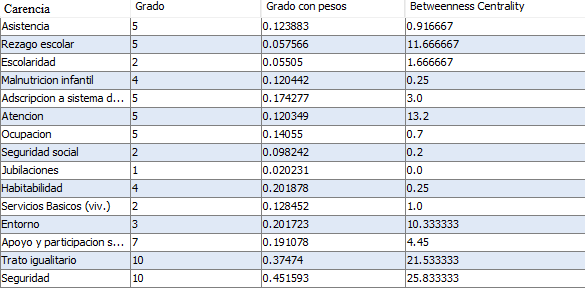
\includegraphics[width=11cm]{analisis grafos/carencias_positivas.png}
    \caption{Resultados análisis de red de correlaciones positivas entre carencias. Elaboración propia.}
    \label{analisisPos}
\end{figure}
%%%%%%%%%%%%%%%%%%%% grafo carencias negativas
\newpage

%%%%%%%%%%%%%%%%%%%%%%%%%%%%%% dimensiones
\newpage
\begin{figure}[H]
  \centering
      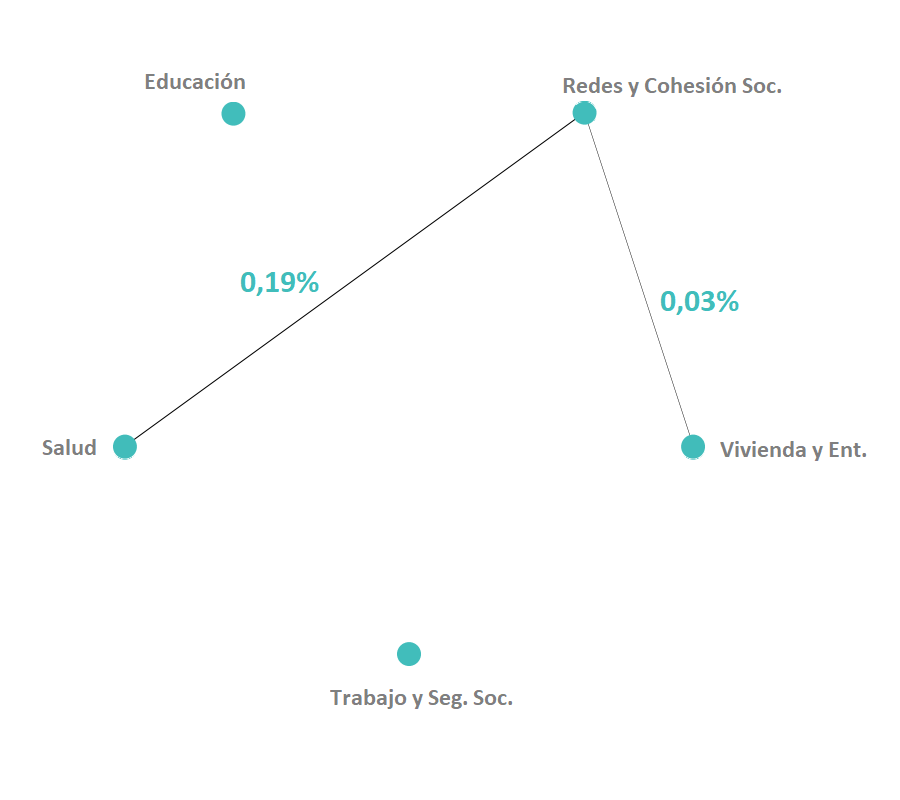
\includegraphics[height=9cm]{Grafos/GrafoDimensiones.png} 
    \caption{Red de dimensiones con coeficientes de correlación positivos. Elaboración propia}
    \label{grafodimpos}
\end{figure}
%%%%%%%%%%%%%%%%%%%%%%%%%%%%%%%
%%%%%%%%%%%%%%%%%%%% analisis dim positivas
\begin{figure}[H]
    \centering
        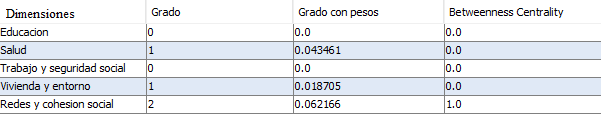
\includegraphics[width=11cm]{analisis grafos/dimensiones_positivas.png}
    \caption{Resultados análisis de red de correlaciones positivas entre dimensiones. Elaboración propia.}
    \label{analisisDIMPOS}
\end{figure}


Poniendo énfasis en los resultados de las correlaciones positivas a nivel de carencias y dimensiones, que son aquellas que afectan los indicadores de la pobreza, se evidencia que las carencias con mayor peso estructural corresponden a Seguridad (0,451593) y Trato igualitario (0,37474), las que a su vez son las carencias con mayor grado de intermediación con 25,83 y 21,53 respectivamente. Es importante recordar que el peso estructural no tiene relación con las causas de la pobreza, sino que expresa, más bien, la importancia que tiene dicha carencia dentro de la red y que permite entender la dinámica interna de la pobreza. En este sentido, se podría decir que las carencias Seguridad y Trato igualitario serían buenos predictores simples para afirmar que en un hogar existe pobreza multidimensional. Del mismo modo, se podría decir que las carencias Seguridad y Trato igualitario son aquellas que permiten reunir a más carencias y de la manera más directa. 

Ahora bien, las dimensiones con mayor peso estructural corresponden a Redes y cohesión social (0,062166) y Salud (0,043461), y la carencia con mayor grado de intermediación corresponde a Redes y cohesión social con 1,00. Esto significa, que las dimensiones Redes y cohesión social y Salud son buenos predictores simples para determinar si un hogar se encuentra en situación de pobreza o no. Del mismo modo, Redes y cohesión social corresponde a la dimensión que reúne a más dimensiones y de la manera más directa.

\end{enumerate}


\subsection{RESULTADOS PARTE II}
%%%%%%%%%%%%%%%%%%%%%%%%%%%%%%%%%%%%%%%%%%%%%%%%%%%%%%%%%%%%%%%%%%%%%%%%%%%%%%%%%%%%%%%%%%%%% Resultados Mati N
En esta segunda etapa, a la muestra de hogares pobres multidimensionales se le aplicó la propiedad de descomposición tomando en cuenta tres criterios (clasificación por tipo de hogar, por zona de residencia y por número de personas que componen el hogar), y se obtuvieron, de este modo, subgrupos de análisis que permitieron focalizar el estudio. También se realizó un análisis comparativo con el nivel de ingresos de los hogares, empleando como medida de referencia la línea de la pobreza.


\subsection{Análisis relacional por tipo de hogar}
La descomposición de la muestra por tipo de hogar generó 6 subgrupos de análisis, que corresponden a los 6 tipos de hogares existentes y que consideran las definiciones especificadas en la sección anterior. Cada subgrupo fue sometido a un análisis relacional, es decir, un cálculo de las correlaciones entre carencias, que permitió obtener un mapa de calor, una red de carencias, los grados nodales y los grados de intermediación de las carencias. 

En la Figura \ref{distHogarTotal} se presenta la distribución de los hogares considerando la muestra total de hogares, y en la Figura \ref{distHogarpobres} se presenta la distribución de los hogares considerando la muestra de hogares pobres multidimensionales. 

\begin{figure}[H]
    \centering
    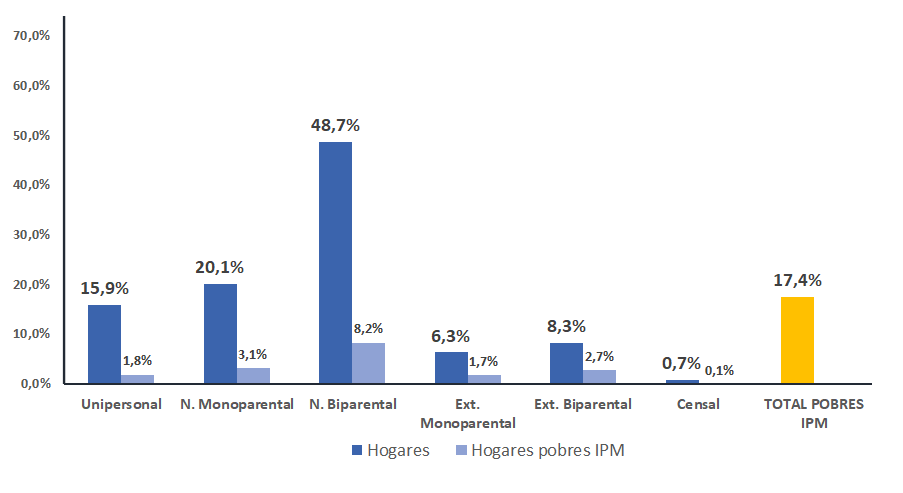
\includegraphics[width=\textwidth]{Max/distribucion_tipo_hogar_casen.png}
    \caption{Distribución por tipo de hogar. Fuente: Elaboración propia.}
    \label{distHogarTotal}
\end{figure}

\begin{figure}[H]
    \centering
    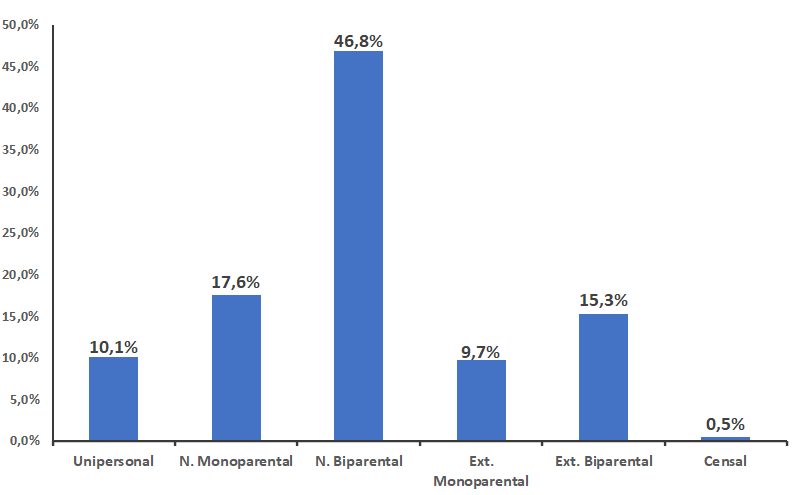
\includegraphics[width=\textwidth]{Max/distribucion_hog_pobres_por_tipo_hogar.png}
    \caption{Distribución por tipo de hogar, hogares pobres multidimensionales. Fuente: Elaboración propia.}
    \label{distHogarpobres}
\end{figure}
Como se puede apreciar, el tipo de hogar biparental nuclear es el más presente en la muestra total y en la muestra de hogares pobres multidimensionales. Mientras que el tipo de hogar censal es el menos presente en la muestra total y en la muestra de hogares pobres multidimensionales. 

A continuación, se detallan los resultados para cada tipo de hogar.

\subsubsection{Análisis relacional Hogar Unipersonal}
El subgrupo de hogares unipersonales tiene un tamaño de muestra de 1.246 hogares, que representan el 10,1\% del total de hogares pobres multidimensionales. En la Figura \ref{freHUni} se presenta un resumen de la distribución de carencias de la muestra.
\begin{figure}[H]
    \centering
        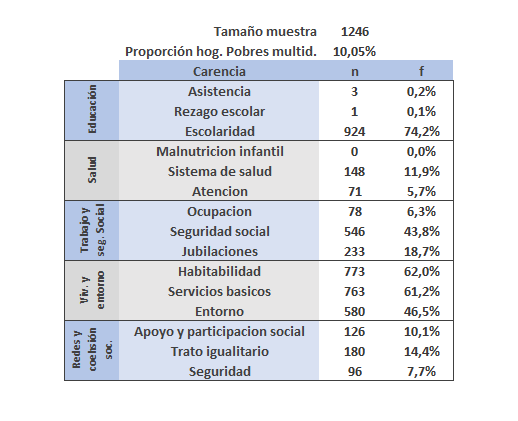
\includegraphics[height=9cm]{HOGARES/tabla_unip.png}
    \caption{Frecuencia de carencias Hogar Unipersonal. Fuente: Elaboración propia.}
    \label{freHUni}
\end{figure}
Como se puede observar, Escolaridad es la carencia más presente en los hogares unipersonales con una frecuencia de 74,2\%. Habitabilidad, Servicios básicos y Entorno, todas pertenecientes a la dimensión Vivienda y entorno, son las otras carencias más frecuentes. La carencia Malnutrición infantil no se encuentra presente en ningún hogar, y las carencias Asistencia Escolar y Rezago Escolar son las carencias menos presentes en los hogares, con frecuencias de 0,2\% y 0,1\% respectivamente. Esto resulta previsible debido a la definición de este tipo de hogar (hogares conformados por un solo integrante), ya que se espera que las personas que viven solas sean adultas. 

En la Figura \ref{HMUni} se presenta el mapa de calor con las correlaciones entre carencias y en las Figuras \ref{RedUnipos} y \ref{RedUniNeg} las redes de correlaciones positivas y negativas respectivamente.
En el mapa de calor, las correlaciones positivas más fuertes se expresan con color azul oscuro y las correlaciones negativas más fuertes se expresan con color rojo intenso. Del mismo modo, en las redes de correlaciones positivas y negativas, las correlaciones más fuertes se expresan con líneas (aristas) más oscuras y gruesas.

\begin{figure}[H]
    \centering
        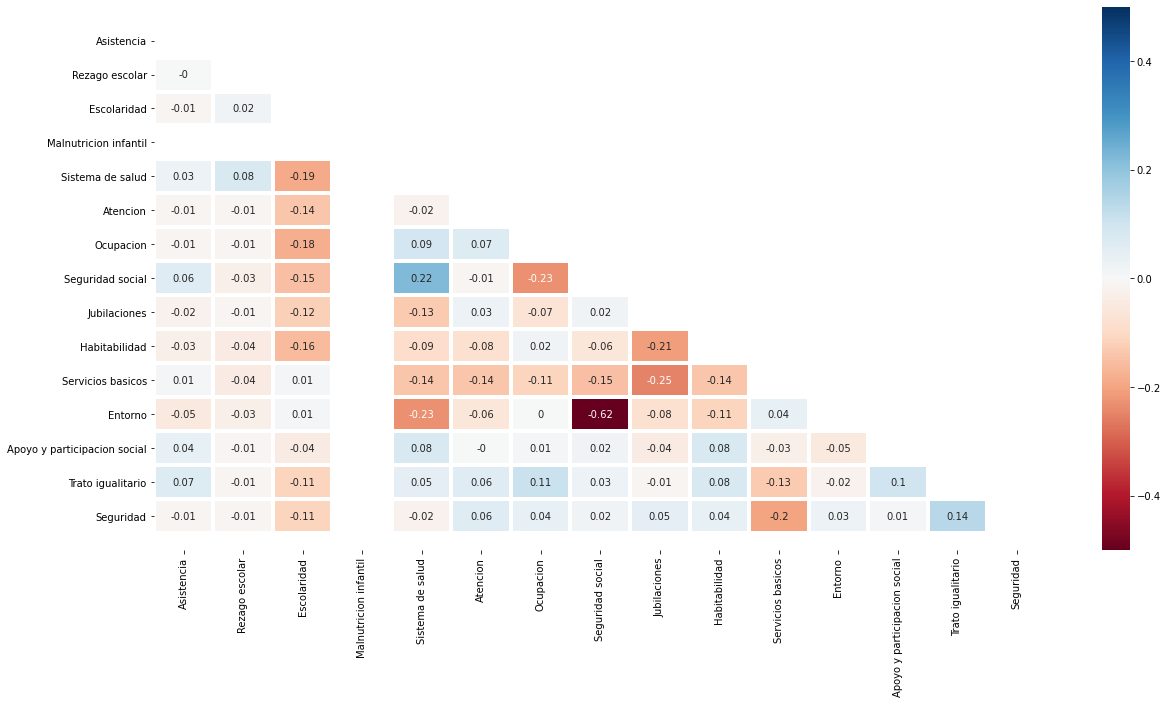
\includegraphics[height=10cm]{Heatmaps/Heatmap_pearson_car_unip.png}
    \caption{Coeficiente de correlación phi entre carencias Hogar unipersonal. Fuente: Elaboración propia.}
    \label{HMUni}
\end{figure}
\begin{figure}[H]
  \centering
    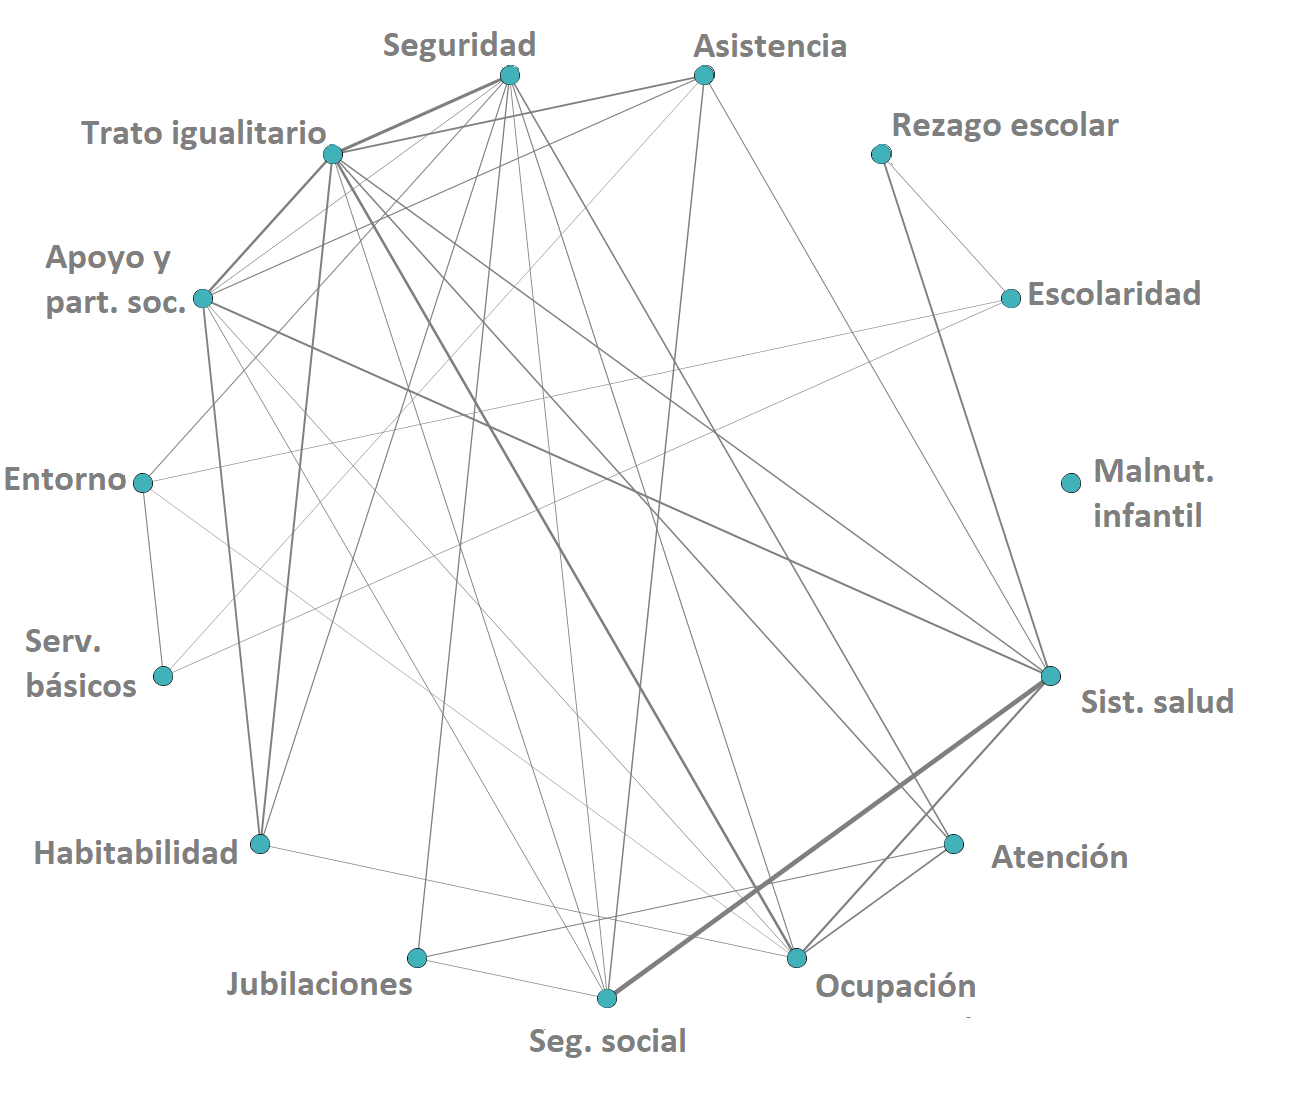
\includegraphics[height=8cm]{Grafos/grafo_unipersonal_pos.png}
    \caption{Red de correlaciones positivas Hogar Unipersonal. Fuente: Elaboración propia.}
    \label{RedUnipos}
\end{figure}
Resulta relevante recordar que un alto grado de correlación positiva entre dos carencias significa que es más común que esas carencias se presenten simultáneamente en un hogar. Mientras que un alto grado de correlación negativa significa que es más común que esas carencias no se presenten simultáneamente en un hogar.  

En el mapa de calor y en las redes de correlaciones se puede observar que las correlaciones positivas más fuertes se presentan entre las carencias Seguridad social y Adscripción a sistema de salud (0,22), Trato igualitario y Seguridad (0,14), Trato igualitario y Ocupación (0,11), y Trato igualitario y Apoyo y participación social (0,1). A su vez, las correlaciones negativas más fuertes se presentan entre las carencias Entorno y Seguridad social (-0,62), Servicios básicos y Jubilaciones (-0,25), Seguridad social y Ocupación (-0,23), Entorno y Sistema de salud (-0,23), Habitabilidad y Jubilaciones (-0,21), y Seguridad y Servicios básicos (-0,2).

En la Figura \ref{CenUni} se muestran los pesos nodales y los grados de intermediación de las carencias de la red de correlaciones positivas.
\begin{figure}[H]
    \centering
    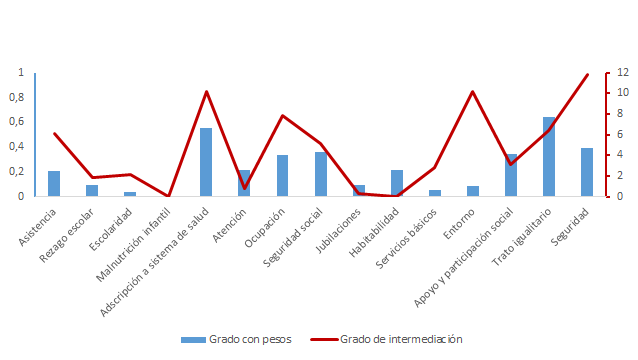
\includegraphics[height=8cm]{Grafos/nc_unipersonal.png}
    \caption{Grados de intermediación y pesos nodales Hogar Unipersonal. Fuente: Elaboración propia.}
    \label{CenUni}
\end{figure}
Los pesos nodales muestran el nivel de conectividad de una carencia con el resto de las carencias de la red, y los grados de intermediación muestran el grado en que una carencia actúa de enlace de otras 2 carencias, reuniendo a más privaciones de la forma más directa. Como se puede apreciar, las carencias con mayor peso nodal son Trato igualitario y Adscripción a sistema de salud, y las carencias con mayor grado de intermediación son Seguridad, Adscripción a sistema de salud y Entorno. 

Si bien Escolaridad es la carencia más presente en los hogares unipersonales, las dinámicas internas de este tipo de hogar sugieren que las carencias Adscripción a sistema de salud, Trato igualitario, Seguridad y Entorno podrían ser predictores simples de que un hogar es pobre multidimensional, debido a los vínculos que generan estas carencias con otras de la red. 

\subsubsection{Análisis relacional Hogar Monoparental Nuclear}
El subgrupo de hogares monoparentales nucleares tiene un tamaño de muestra de 2.180 hogares, que representan el 17,6\% del total de hogares pobres multidimensionales. En la Figura \ref{freHMononuc} se muestran las distribuciones de las carencias.
\begin{figure}[H]
  \centering
    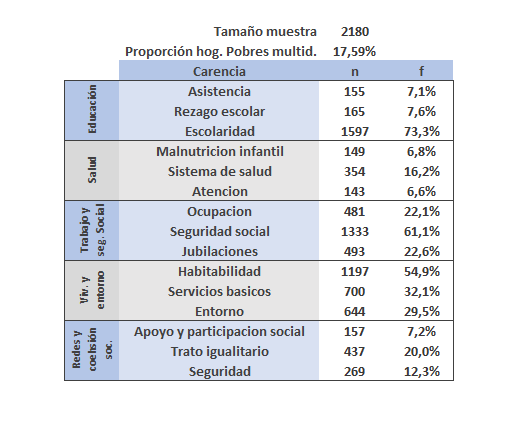
\includegraphics[height=9cm]{HOGARES/tabla_mononuc.png}
    \caption{Frecuencia carencias Hogar Monoparental Nuclear. Fuente: Elaboración propia.}
    \label{freHMononuc}
\end{figure}
Como se puede observar, las carencias más frecuentes en este subgrupo son Escolaridad, Seguridad social y Habitabilidad con frecuencias de 73,3\%, 61,1\% y 54,9\% respectivamente. Mientras que las carencias menos frecuentes son Atención, Malnutrición infantil, Asistencia escolar, Apoyo y participación social y Rezago escolar.

En la Figura \ref{HM_HMononuc} se presenta el mapa de calor con las correlaciones entre carencias, y en las Figuras \ref{RedMononucpos} y \ref{RedMononucneg} las redes de correlaciones positivas y negativas respectivamente.

\begin{figure}[H]
    \centering
    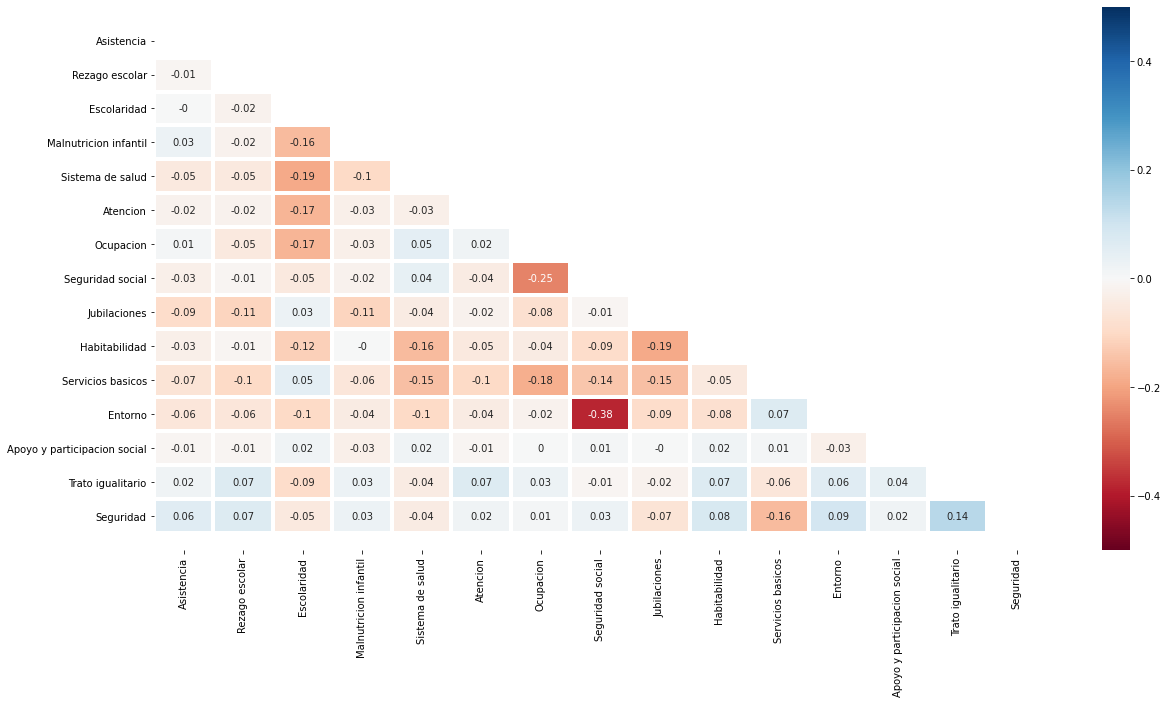
\includegraphics[height=10cm]{Heatmaps/Heatmap_pearson_car_monuc.png}
    \caption{Coeficiente de correlación phi entre carencias Hogar Monoparental Nuclear. Fuente: Elaboración propia.}
    \label{HM_HMononuc}
\end{figure}

\begin{figure}[H]
  \centering

    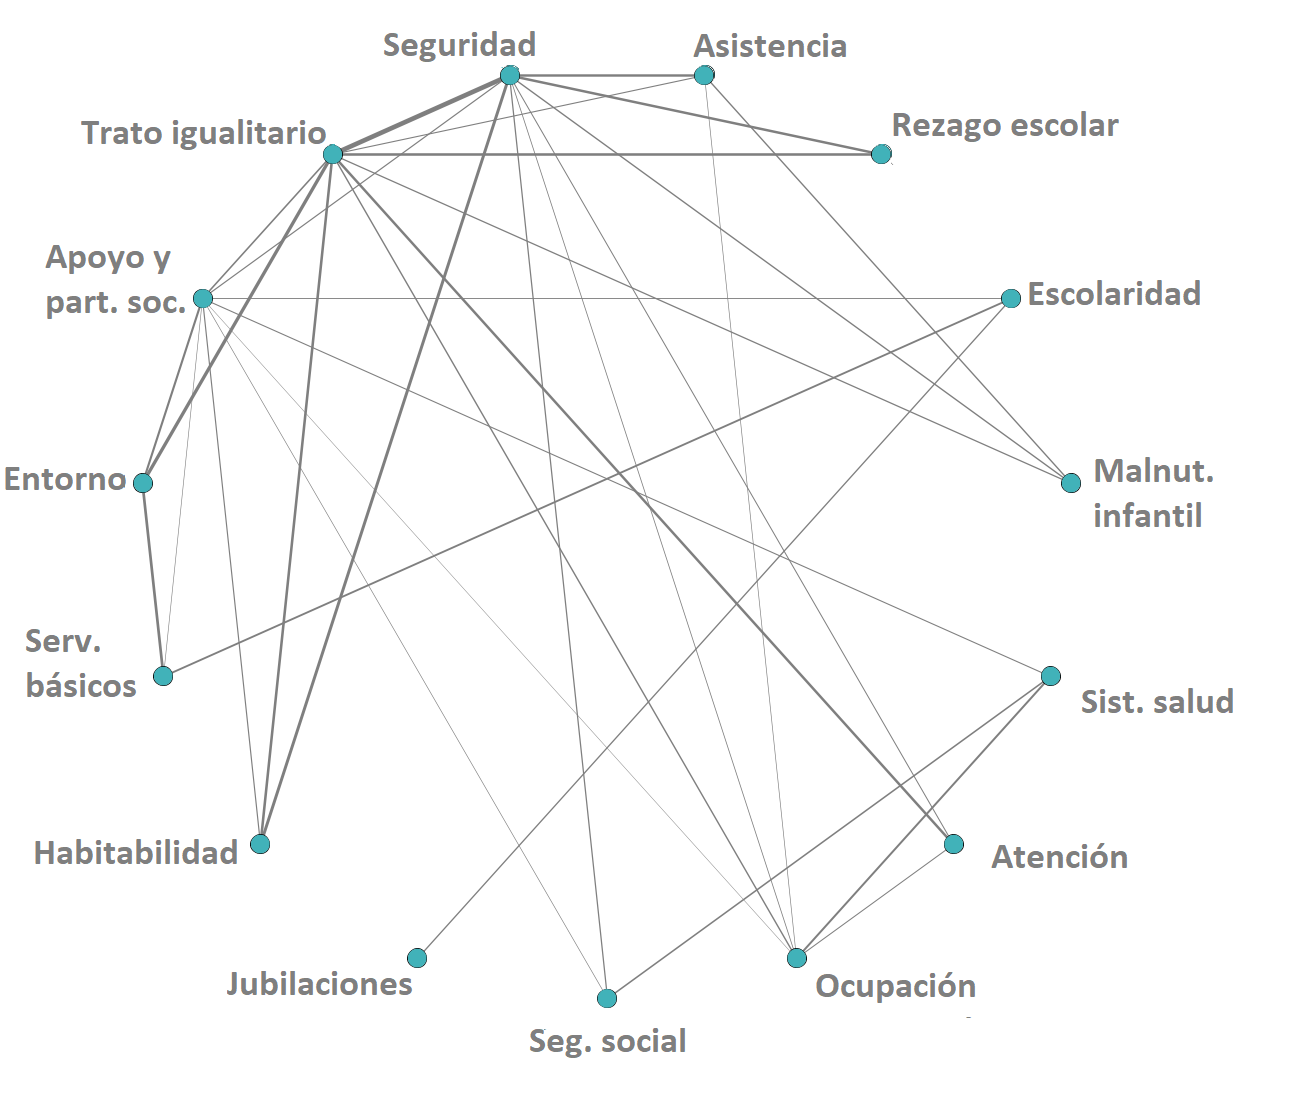
\includegraphics[width=10cm]{Grafos/grafo_mononuc_pos.png}
    \caption{Red de correlaciones positivas Hogar Monoparental Nuclear. Fuente: Elaboración propia.}
    \label{RedMononucpos}

\end{figure}

Las correlaciones positivas más fuertes se presentan entre las carencias Seguridad y Trato igualitario (0,14), Seguridad y Entorno (0,09), y Seguridad y Habitabilidad (0,08). Las correlaciones negativas más fuertes se presentan entre las carencias Entorno y Seguridad social (-0,38), Seguridad social y Ocupación (-0,25), Sistema de salud y Escolaridad (-0,19), y Habitabilidad y Jubilaciones (-0,19).

En la Figura \ref{CenMononuc} se presentan los pesos nodales y grados de intermediación de la red de correlaciones positiva.
\begin{figure}[H]
    \centering
    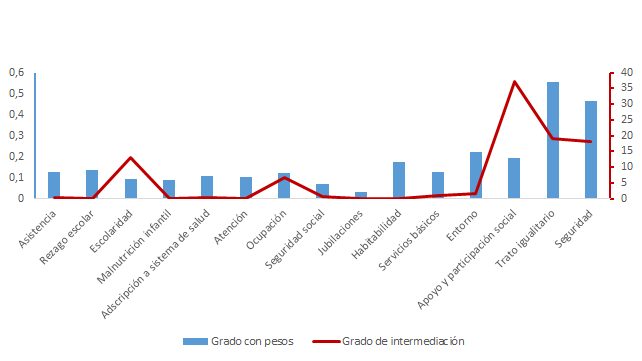
\includegraphics[height=8cm]{Grafos/nc_mononuc.png}
    \caption{Grados de intermediación y pesos nodales Hogar Monoparental Nuclear. Fuente: Elaboración propia.}
    \label{CenMononuc}
\end{figure}
Las carencias con mayor peso nodal son Trato igualitario (0,55) y Seguridad (0,46), y las carencias con mayor grado de intermediación son Apoyo y participación social (37,06), Trato igualitario (19,06), y Seguridad (18,1).

Las carencias Apoyo y participación social, Trato igualitario y Seguridad, pertenecientes a la dimensión Redes y cohesión social, son las que están más conectadas con el resto de las carencias de la red, y su manifestación en este tipo de hogar se considera un predictor simple para determinar que un hogar es pobre multidimensional.  

\subsubsection{Análisis relacional Hogar Biparental Nuclear}
El subgrupo de los hogares biparentales nucleares tiene un tamaño de muestra de 5.804 hogares, que representan el 46,8\% del total de hogares pobres multidimensionales. En la Figura \ref{freBinuc} se presentan las distribuciones de las carencias.
\begin{figure}[H]
  \centering
    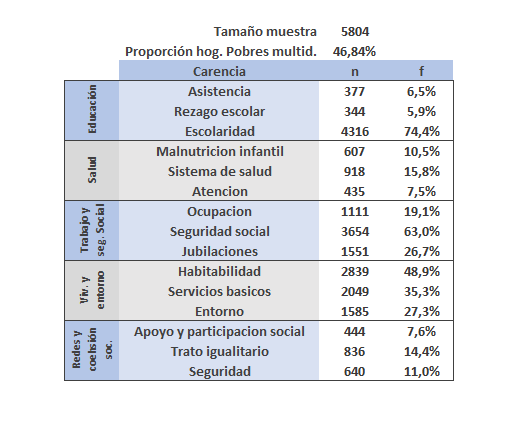
\includegraphics[height=9cm]{HOGARES/tabla_binuc.png}
    \caption{Frecuencia de carencias Hogar Biparental Nuclear. Fuente: Elaboración propia.}
    \label{freBinuc}
\end{figure}
Las carencias más frecuentes son Escolaridad, Seguridad social y Habitabilidad con frecuencias de 74,4\%, 63\% y 48,9\% respectivamente. Mientras que las carencias menos frecuentes son Rezago escolar, Asistencia escolar, Atención de salud y Apoyo y participación social con frecuencias de 5,9\%, 6,5\% y 7,5\% respectivamente.

En la Figura \ref{HMBinuc} se presentan las correlaciones entre carencias y en las Figuras \ref{RedBinucpos} y \ref{RedBinucneg} las redes de correlaciones positivas y negativas respectivamente.
\begin{figure}[H]
    \centering
    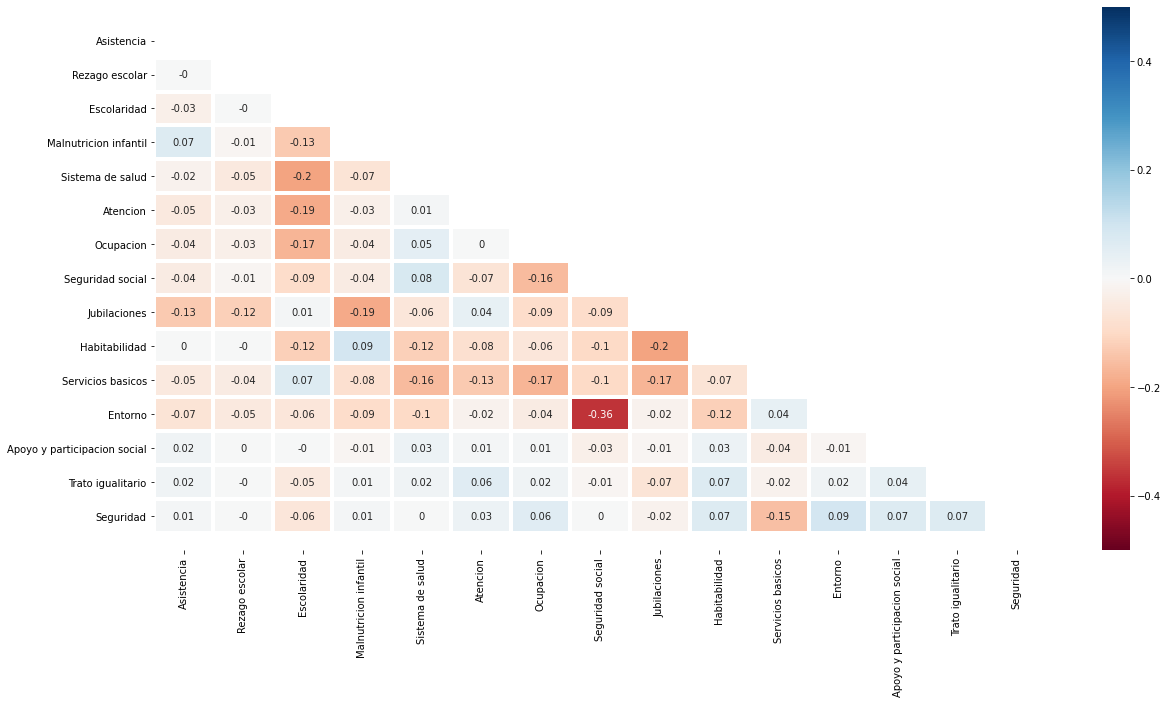
\includegraphics[height=10cm]{Heatmaps/Heatmap_pearson_car_binuc.png}
    \caption{Coeficiente de correlación phi entre carencias Hogar Biparental Nuclear. Fuente: Elaboración propia.}
    \label{HMBinuc}
\end{figure}

\begin{figure}[H]
  \centering
    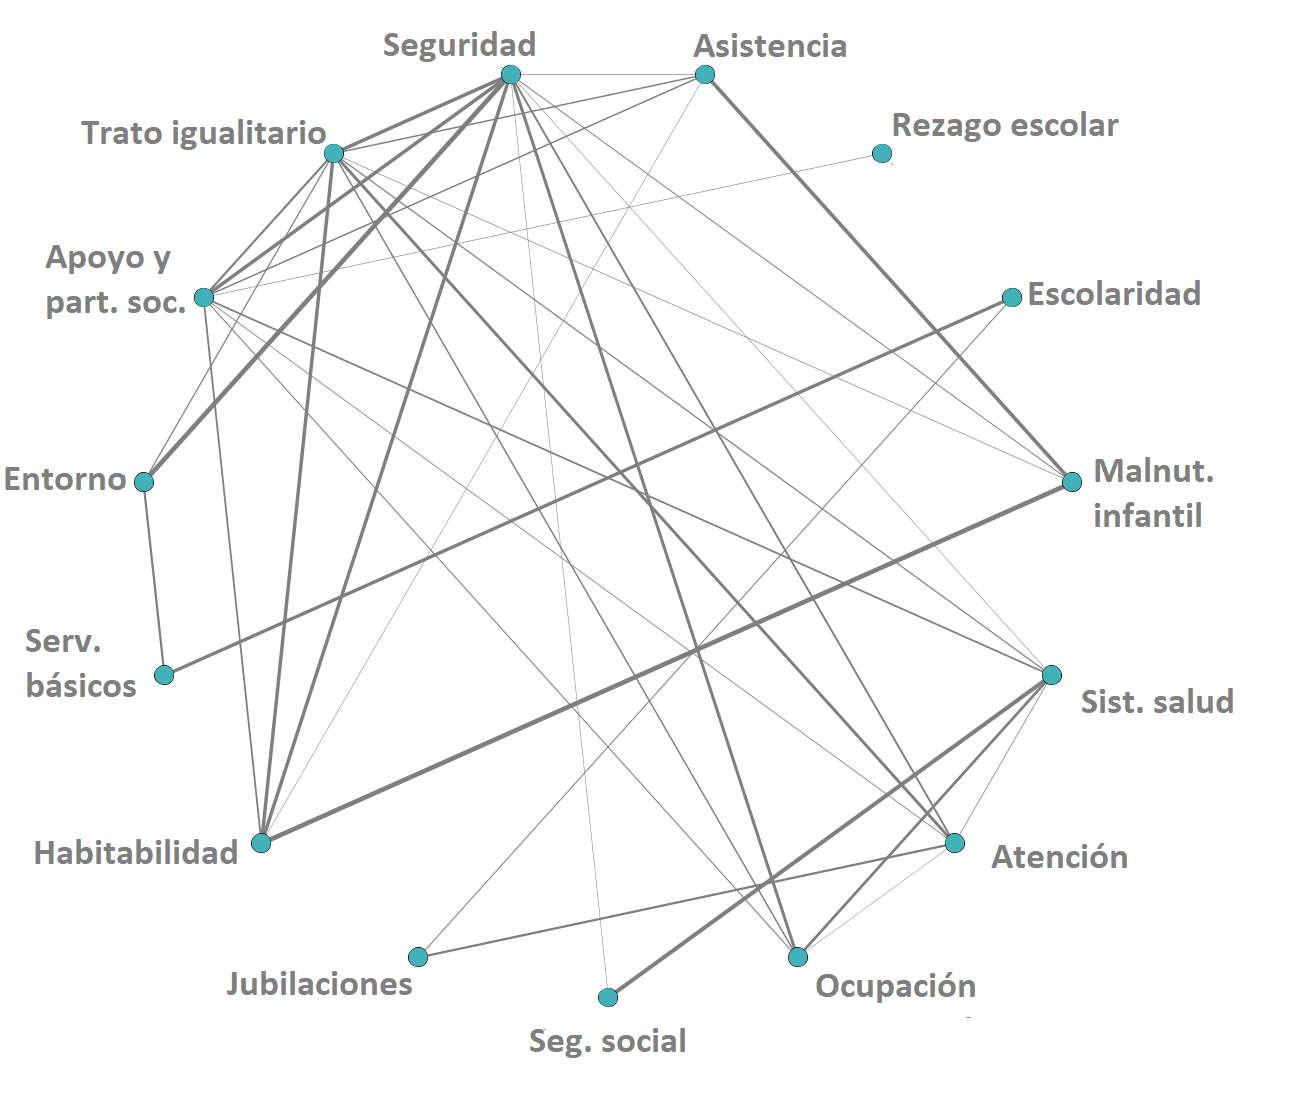
\includegraphics[width=10cm]{Grafos/grafo_binuc_pos.png}
    \caption{Red de correlaciones positivas Hogar Biparental Nuclear. Fuente: Elaboración propia.}
    \label{RedBinucpos}
\end{figure}

Las correlaciones positivas más fuertes se presentan entre las carencias Habitabilidad y Malnutrición infantil (0,09), Seguridad y Entorno (0,09), y Seguridad social y Sistema de salud (0,08). Las correlaciones negativas más fuertes se presentan entre las carencias Entorno y Seguridad social (-0,36), Sistema de salud y Escolaridad (-0,2), y Habitabilidad y Jubilaciones (-0,2).

En la Figura \ref{CenBinuc} se muestran los pesos nodales y los grados de intermediación de la red de correlaciones positiva. 
\begin{figure}[H]
    \centering
    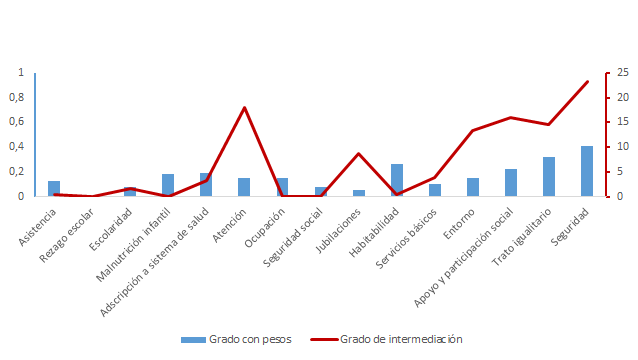
\includegraphics[width=\textwidth]{Grafos/nc_binuc.png}
    \caption{Grados de intermediación y pesos nodales Hogar Biparental Nuclear. Fuente: Elaboración propia.}
    \label{CenBinuc}
\end{figure}
Las carencias con mayor peso nodal son Seguridad (0,41) y Trato igualitario (0,32). Mientras que las carencias con mayor grado de intermediación son Seguridad (23,3), Atención de salud (18,03), Apoyo y participación social (16,06) y Trato igualitario (14,63).

Las carencias Apoyo y participación social, Trato igualitario y Seguridad, pertenecientes a la dimensión Redes y cohesión social, y Atención de salud, son las que están más conectadas con otras carencias, lo que permite que actúen como predictores simples en este tipo de hogar para identificar a un hogar pobre multidimensional.  

\subsubsection{Análisis relacional Hogar Monoparental Extendido}

El subgrupo de hogares monoparentales extendidos comprende 1.202 hogares, que representan el 9,7\% del total de hogares pobres multidimensionales. En la Figura \ref{freMonoex} se muestran las distribuciones de las carencias.

\begin{figure}[H]
  \centering
    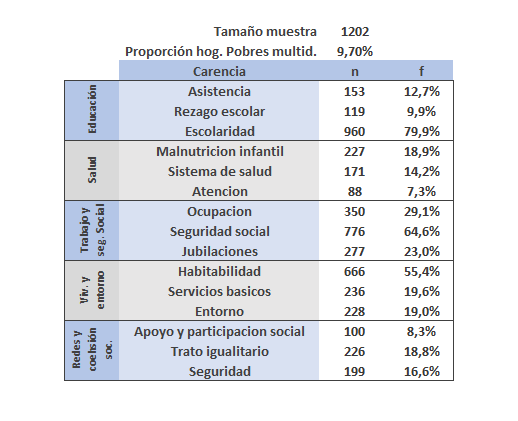
\includegraphics[height=9cm]{HOGARES/tabla_monoex.png}
    \caption{Frecuencia de carencias Hogar Monoparental Extendido. Fuente: Elaboración propia.}
    \label{freMonoex}
\end{figure}
Como se puede observar, las carencias más frecuentes son Escolaridad, Seguridad social y Habitabilidad, con frecuencias de 79,9\%, 64,6\% y 55,4\% respectivamente. Las carencias menos frecuentes son Atención de salud, Apoyo y participación social, y Rezago escolar.

En la Figura \ref{HMMonoex} se presenta el mapa de calor de las correlaciones entre carencias y en las Figuras \ref{RedMonoexpos} y \ref{RedMonoexneg} las redes de correlaciones positivas y negativas respectivamente.

\begin{figure}[H]
    \centering
    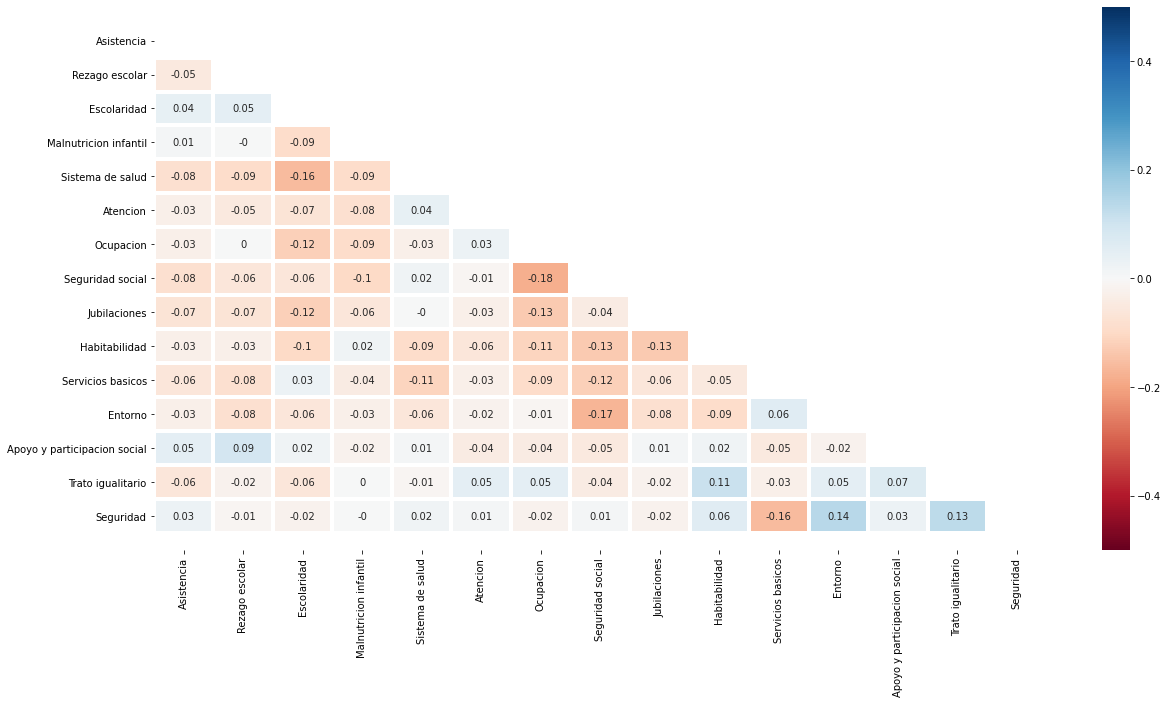
\includegraphics[height=10cm]{Heatmaps/Heatmap_pearson_car_monoex.png}
    \caption{Coeficiente de correlación phi entre carencias Hogar Monoparental Extendido. Fuente: Elaboración propia.}
    \label{HMMonoex}
\end{figure}

\begin{figure}[H]
  \centering
    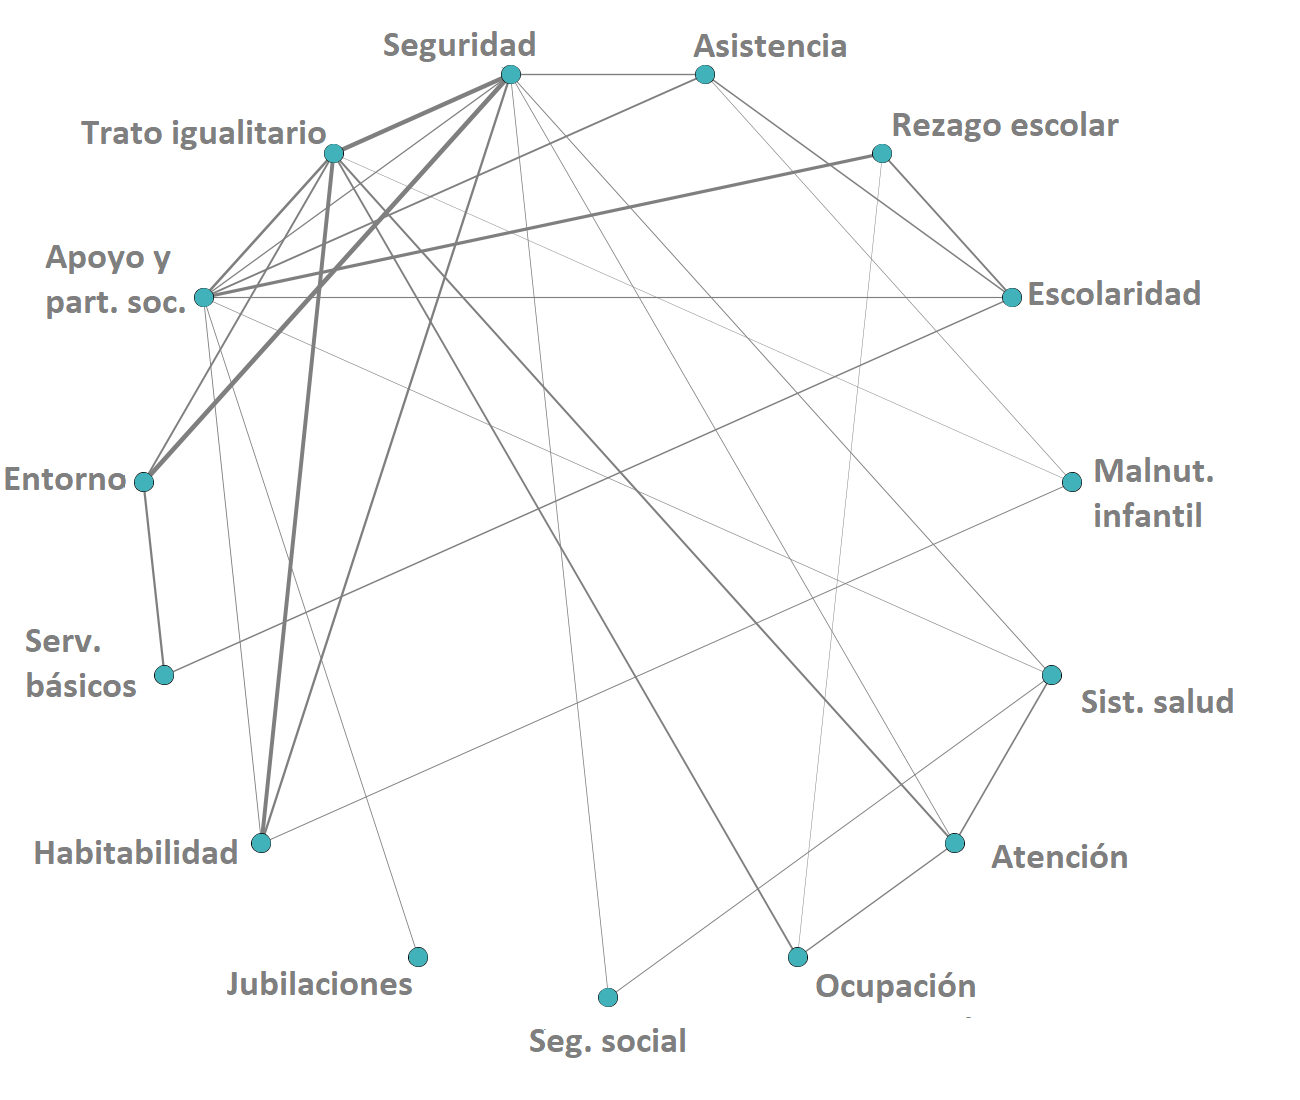
\includegraphics[width=10cm]{Grafos/grafo_monoex_pos.png}
    \caption{Red de correlaciones positivas Hogar Monoparental Extendido. Fuente: Elaboración propia.}
    \label{RedMonoexpos}
\end{figure}
Las correlaciones positivas más fuertes se presentan entre las carencias Seguridad y Entorno (0,14), Seguridad y Trato igualitario (0,13) y Trato igualitario y Habitabilidad (0,11). Las correlaciones negativas más fuertes se manifiestan entre las carencias Seguridad social y Ocupación (-0,18), Entorno y Seguridad social (-0,17), Sistema de salud y Escolaridad (-0,16) y Seguridad y Servicios básicos (-0,16). 

En la Figura \ref{CenMonoex} se muestran los pesos nodales y grados de intermediación de la red de correlaciones positiva.

\begin{figure}[H]
    \centering
    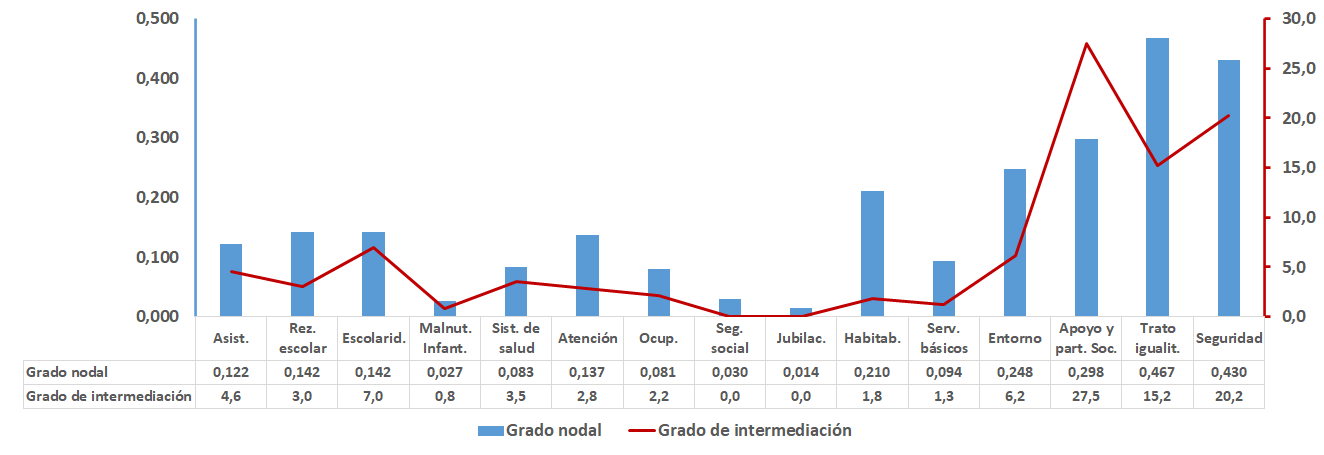
\includegraphics[width=\textwidth]{Grafos/nc_monoex.png}
    \caption{Grados de intermediación y pesos nodales Hogar Monoparental Extendido. Fuente: Elaboración propia.}
    \label{CenMonoex}
\end{figure}
Las carencias con mayor peso nodal son Trato igualitario (0,46) y Seguridad (0,43) y las carencias con mayor grado de intermediación son Apoyo y participación social (27,46), Seguridad (20,24) y Trato igualitario (15,19).

Las carencias Apoyo y participación social, Trato igualitario y Seguridad, pertenecientes a la dimensión Redes y cohesión social, son las que presentan más conexiones con el resto de las carencias de la red, por lo que su manifestación en este tipo de hogar podría considerarse un predictor simple de que el hogar es pobre multidimensional.


\subsubsection{Análisis relacional Hogar Biparental Extendido}

El subgrupo de hogares biparentales extendidos tiene un tamaño de 1.894 hogares, que representan el 15,3\% de los hogares pobres multidimensionales. En la Figura \ref{freBiex} se muestran las distribuciones de las carencias.

\begin{figure}[H]
  \centering
    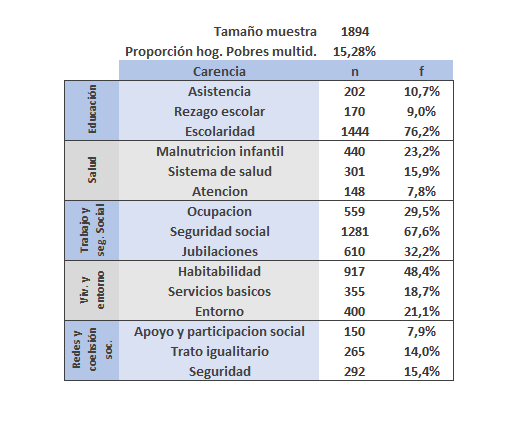
\includegraphics[height=9cm]{HOGARES/tabla_biex.png}
    \caption{Frecuencia de carencias Hogar Biparental Extendido. Fuente: Elaboración propia.}
    \label{freBiex}
\end{figure}

Como se puede apreciar, las carencias más frecuentes son Escolaridad (76,2\%), Seguridad social (67,6\%) y Habitabilidad (48,4\%). Las carencias menos frecuentes son Atención de salud (7,8\%), Apoyo y participación social (7,9\%) y Rezago escolar (9,0\%).

En la Figura \ref{HMBiex} se presenta un mapa de calor de las correlaciones entre carencias y en las Figuras \ref{RedBiexpos} y \ref{RedBiexneg} las redes de correlaciones positivas y negativas respectivamente.

\begin{figure}[H]
    \centering
    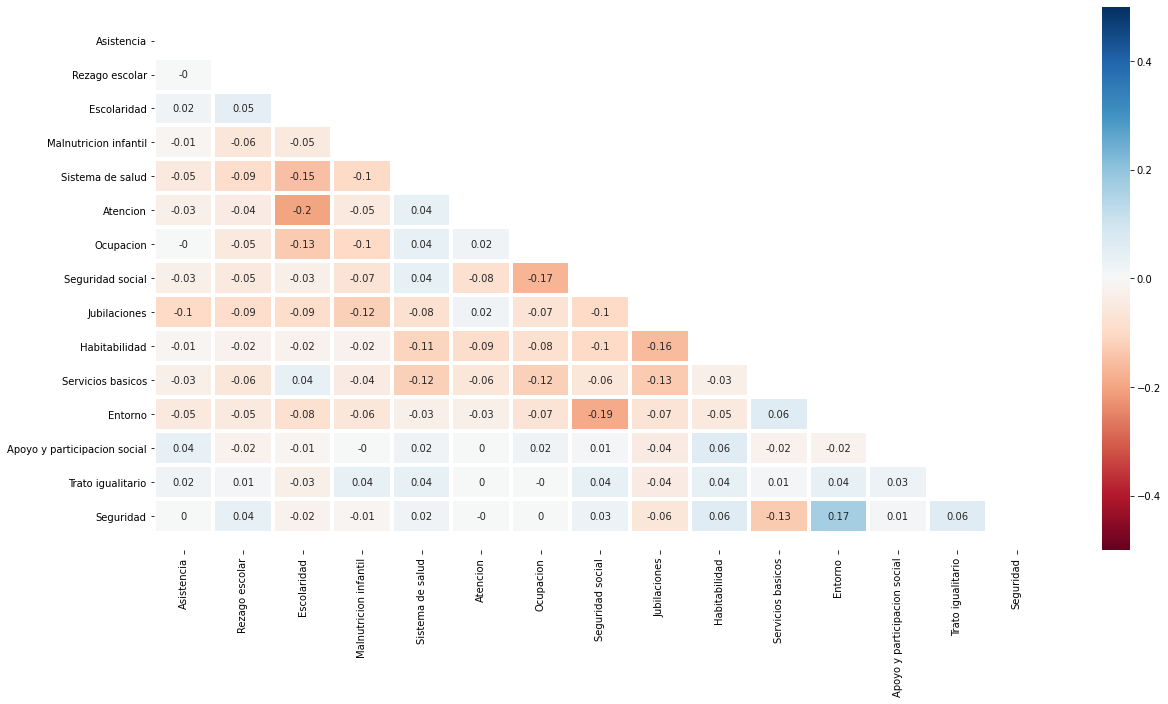
\includegraphics[width=\textwidth]{Heatmaps/Heatmap_pearson_car_biex.png}
    \caption{Coeficiente de correlación phi entre carencias Hogar Biparental Extendido. Fuente: Elaboración propia.}
    \label{HMBiex}
\end{figure}

\begin{figure}[H]
  \centering
    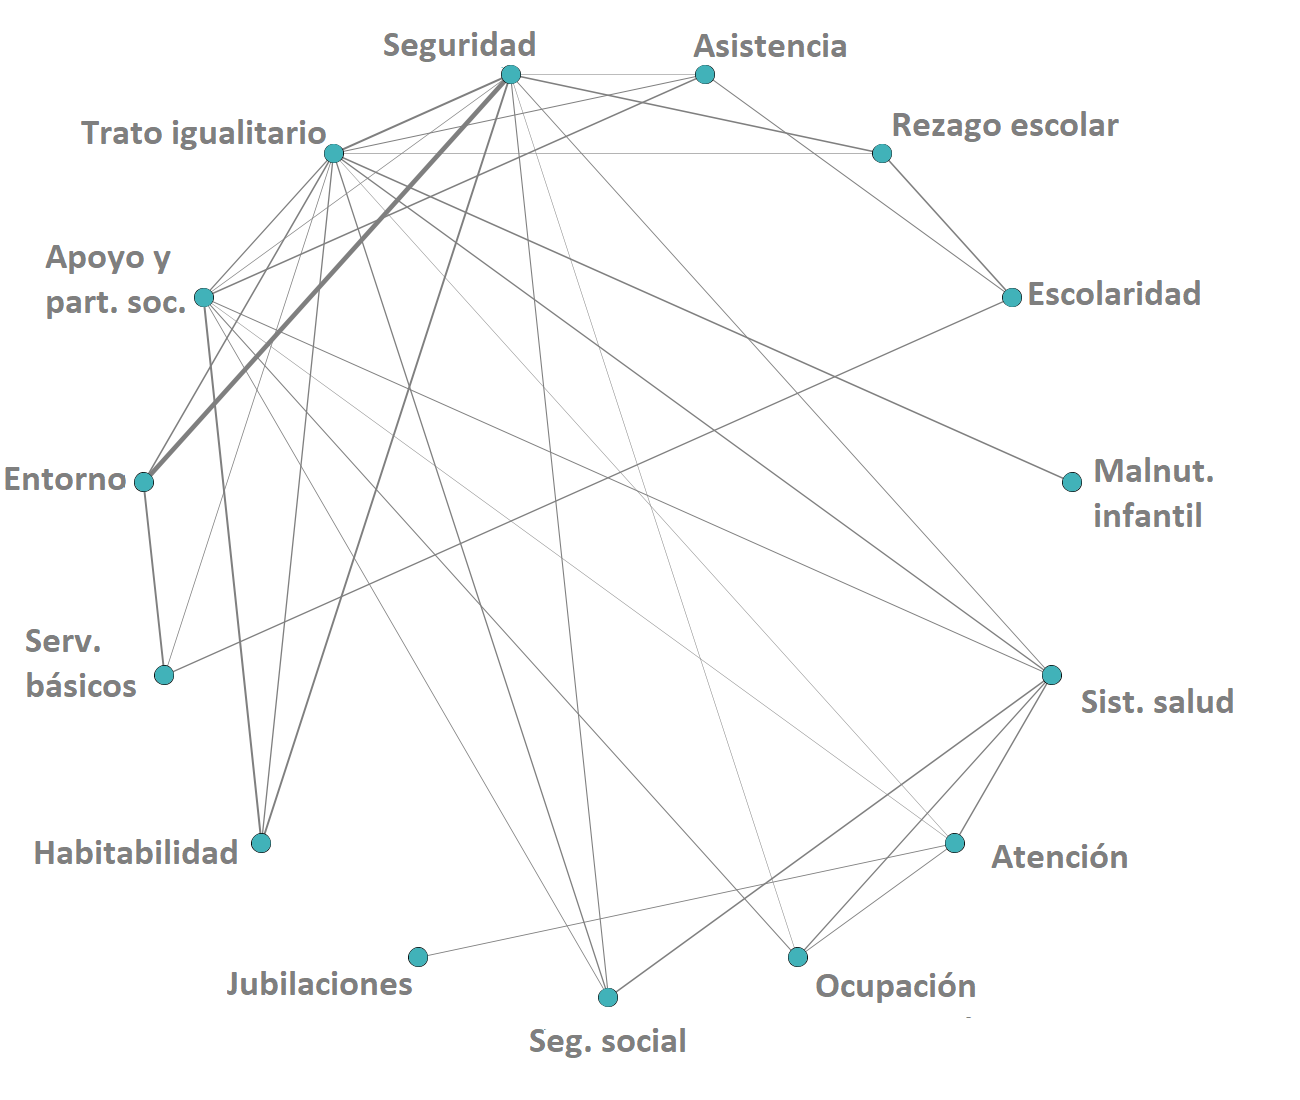
\includegraphics[width=10cm]{Grafos/grafo_biex_pos.png}
    \caption{Red de correlaciones positivas Hogar Biparental Extendido. Fuente: Elaboración propia.}
    \label{RedBiexpos}
\end{figure}

La correlación positiva más fuerte se presenta entre las carencias Seguridad y Entorno (0,17). Y las correlaciones negativas más fuertes se presentan entre las carencias Atención de salud y Escolaridad (-0,2), Entorno y Seguridad social (-0,19), y Seguridad social y Ocupación (-0,17).

En la Figura \ref{CenBiex} se muestran los pesos nodales y grados de intermediación de las carencias de la red de correlaciones positivas.

\begin{figure}[H]
    \centering
    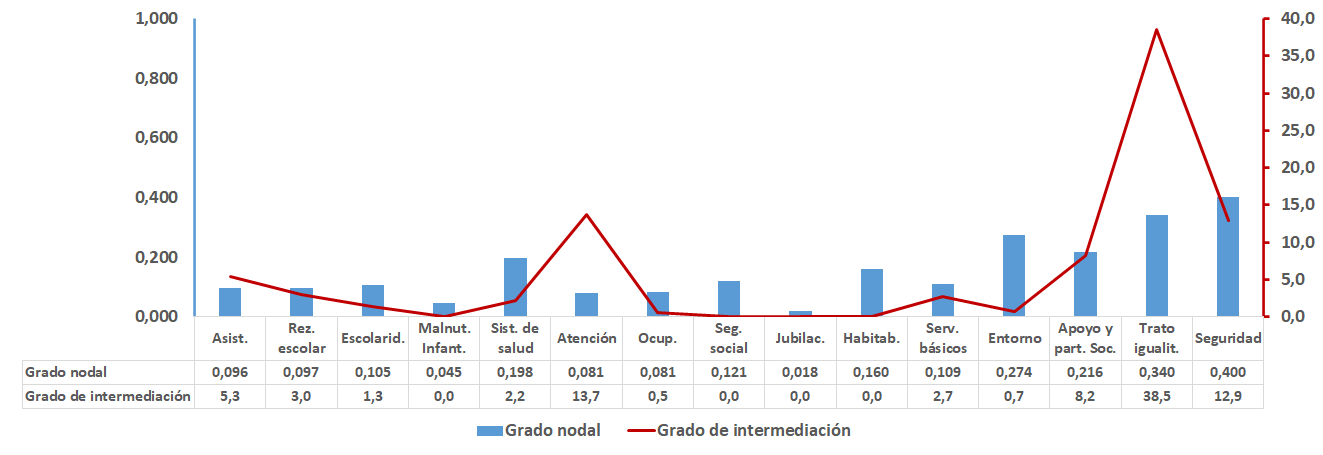
\includegraphics[width=\textwidth]{Grafos/nc_biex.png}
    \caption{Grados de intermediación y pesos nodales Hogar Biparental Extendido. Fuente: Elaboración propia.}
    \label{CenBiex}
\end{figure}
Las carencias con mayor peso nodal son Seguridad (0,40), Trato igualitario (0,34) y Entorno (0,27). Las carencias con mayor grado de intermediación son Trato igualitario (38,47), Atención de salud (13,7) y Seguridad (12,9).

Trato igualitario, Seguridad, Atención de salud y Entorno son las carencias más conectadas con el resto de las carencias de la red, por lo que su manifestación en este tipo de hogar podría considerarse un predictor simple de que dicho hogar es pobre multidimensional. 

\subsubsection{Análisis relacional Hogar Censal}
El subgrupo de hogares censales comprende 66 hogares, que representan el 0,5\% del total de hogares pobres multidimensionales. En la Figura \ref{freCensal} se presenta la distribución de carencias de la muestra.
\begin{figure}[H]
  \centering
    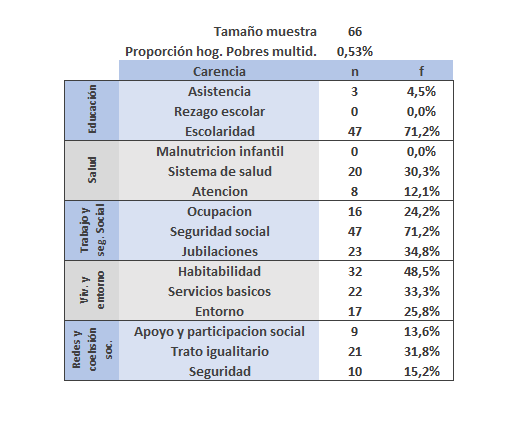
\includegraphics[height=9cm]{HOGARES/tabla_censal.png}
    \caption{Frecuencia de carencias Hogar Censal. Fuente: Elaboración propia.}
    \label{freCensal}
\end{figure}
Como se puede apreciar, las carencias más frecuentes son Escolaridad y Seguridad social, ambas con frecuencias de 71,2\%. Las carencias Rezago escolar y Malnutrición infantil no se encuentran presentes en ningún hogar, y Asistencia escolar es la carencia menos frecuente, lo que resulta previsible considerando la definición de hogar censal, ya que se espera que los integrantes de este tipo de hogar no sean niños. 

En la Figura \ref{HMCensal} se presenta el mapa de calor de las correlaciones entre carencias y en las Figuras \ref{RedCensalpos} y \ref{RedCensalneg} las redes de correlaciones positivas y negativas respectivamente.

\begin{figure}[H]
    \centering
    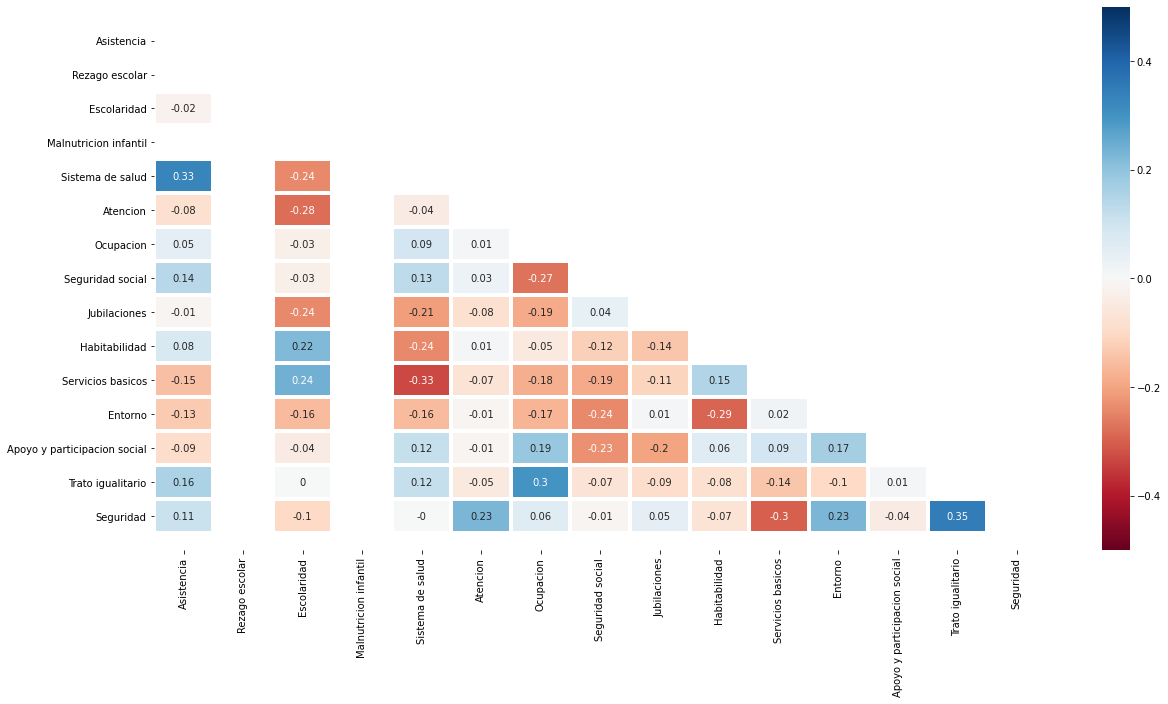
\includegraphics[width=\textwidth]{Heatmaps/Heatmap_pearson_car_censal.png}
    \caption{Coeficiente de correlación phi entre carencias Hogar Censal. Fuente: Elaboración propia.}
    \label{HMCensal}
\end{figure}

\begin{figure}[H]
  \centering
    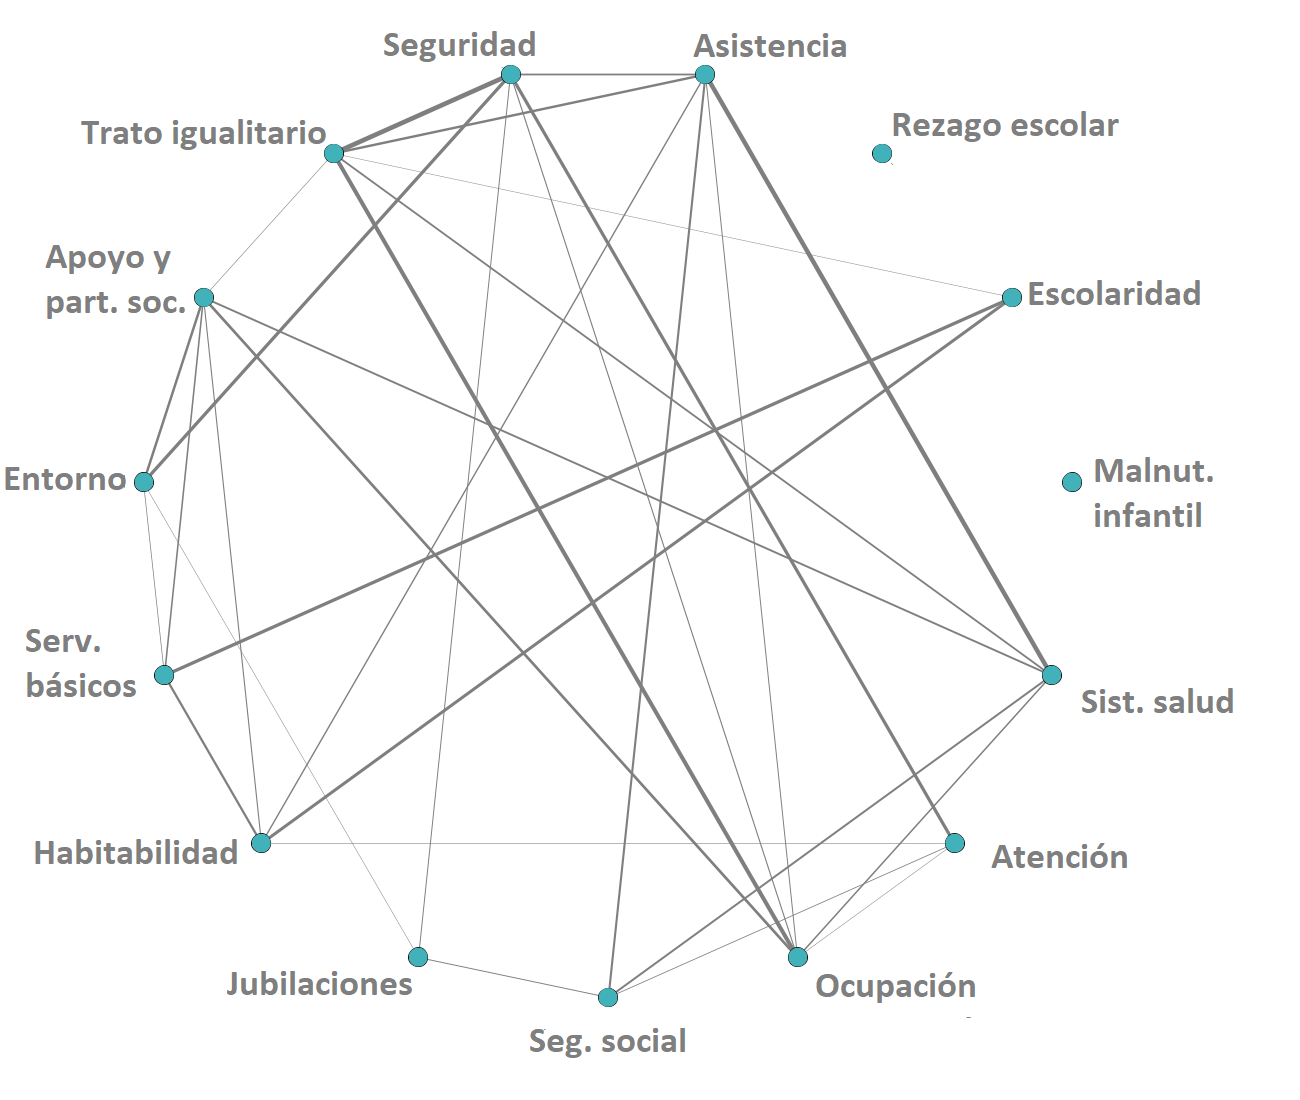
\includegraphics[width=10cm]{Grafos/grafo_censal_pos.png}
    \caption{Red de correlaciones positivas Hogar Censal. Fuente: Elaboración propia.}
    \label{RedCensalpos}
\end{figure}


Las correlaciones positivas más fuertes se presentan entre las carencias Seguridad y Trato igualitario (0,35), Sistema de salud y Asistencia escolar (0,33) y Ocupación y Trato igualitario (0,3). Mientras que las carencias con las correlaciones negativas más fuertes se presentan entre las carencias Servicios básicos y Sistema de salud (-0,33), Seguridad y Servicios básicos (-0,3) y Entorno y Habitabilidad (-0,29). 

En la Figura \ref{CenCensal} se muestra un gráfico con los pesos nodales y grados de intermediación de las carencias de la red de correlaciones positiva.

\begin{figure}[H]
    \centering
    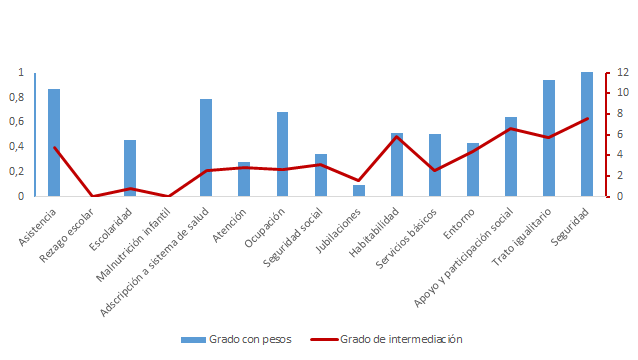
\includegraphics[width=\textwidth]{Grafos/nc_censal.png}
    \caption{Grados de intermediación y pesos nodales Hogar Censal. Fuente: Elaboración propia.}
    \label{CenCensal}
\end{figure}
Las carencias con mayor peso nodal son Seguridad (1,03), Trato igualitario (0,94) y Asistencia escolar (0,87). Las carencias con mayor grado de intermediación son Seguridad (7,58) y Apoyo y participación social (6,58).

Las carencias Seguridad, Trato igualitario, Apoyo y participación social, y Asistencia escolar son las que presentan mayor cantidad de conexiones con el resto de las carencias de la red, por lo que su manifestación en este tipo de hogar podría considerarse un predictor simple de que el hogar es pobre multidimensional. 




\subsection{Análisis tipológico de la pobreza multidimensional}
Las tipologías de las carencias son combinaciones específicas de carencias que se manifiestan en los hogares. Su identificación permite conocer cómo la pobreza afecta a los hogares pobres multidimensionales a través de las privaciones. En la Figura \ref{TipGen} se muestran las tipologías más frecuentes de la muestra original de hogares pobres multidimensionales.
\begin{figure}[H]
    \centering
    \includegraphics[width=\textwidth]{Mati N/tipologíaGeneral.png}
    \caption{Tipologías de carencias más frecuentes de los hogares pobres multidimensionales. Fuente: Elaboración propia.}
    \label{TipGen}
\end{figure}
Como se puede observar, existen 1.849 tipologías de carencias en los hogares pobres multidimensionales, y las 10 más frecuentes representan el 24,59\% de los hogares. Dentro de los aspectos importantes que se desprenden de estas tipologías, destaca la incidencia que tiene Escolaridad, que se condice con las altas frecuencias que presenta en todos los tipos de hogares, y la ausencia de las carencias de la dimensión Redes y cohesión social, que en los análisis por tipo de hogar presentan las centralidades más importantes. Esto último refleja la diferencia que existe entre la aproximación estadística y relacional. También resulta importante notar que el 80\% de las tipologías presenta un \textit{IPM} de 22,5\%, lo que significa que los hogares son pobres multidimensionales en el margen, con la cantidad de carencias mínimas.

Luego de obtener las tipologías de los hogares pobres multidimensionales, se aplicó la propiedad de descomposición tomando en cuenta el número de personas que habitan en un hogar y la zona de residencia, criterios que para efectos de este trabajo son considerados factores externos, ya que no afectan el cálculo del índice de pobreza multidimensional (\textit{IPM}).

\subsubsection{Análisis tipológico por número de personas en el hogar}
La descomposición de la muestra de hogares pobres multidimensionales por número de personas en el hogar generó 7 subgrupos de análisis, los cuales fueron analizados considerando las tipologías y las frecuencias de las carencias. 

A continuación, se detallan los resultados para cada subgrupo.
\begin{itemize}
    \item \textbf{Hogares de 1 integrante}

    El subgrupo de hogares de 1 integrante es idéntico al subgrupo de hogares unipersonales analizado en la sección anterior. Reúne a 1.246 hogares que representan el 10,05\% de los hogares pobres multidimensionales. En las Figuras \ref{fren1} y \ref{tipn1} se presentan las frecuencias y tipologías de las carencias respectivamente. 

    \begin{figure}[H]
        \centering 
        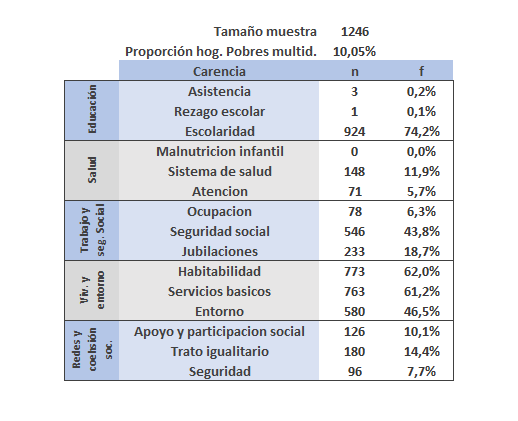
\includegraphics[height=9cm]{HOGARES/tabla_unip.png}
        \caption{Frecuencias de las carencias Hogares de 1 integrante. Fuente: Elaboración propia.}
        \label{fren1}
    \end{figure}
    \begin{figure}[H]
        \centering
        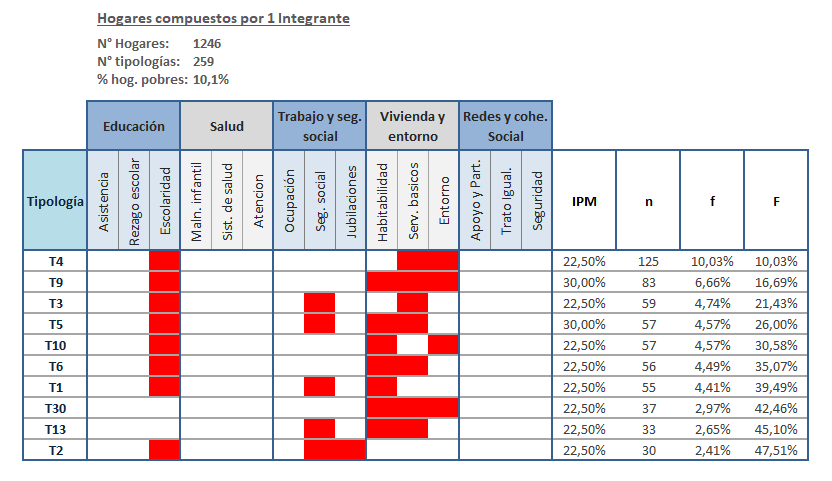
\includegraphics[width=\textwidth]{Mati N/n=1.png}
        \caption{Tipologías más frecuentes Hogares de 1 integrante. Fuente: Elaboración propia.}
        \label{tipn1}
    \end{figure}
    Escolaridad es la carencia más presente en los hogares unipersonales con una frecuencia de 74,2\%. Habitabilidad, Servicios básicos y Entorno, todas pertenecientes a la dimensión Vivienda y entorno, son las otras carencias más frecuentes. La carencia Malnutrición infantil no se encuentra presente en ningún hogar, y las carencias Asistencia Escolar y Rezago Escolar son las carencias menos presentes en los hogares, con frecuencias de 0,2\% y 0,1\% respectivamente. Esto resulta previsible debido a la definición de este tipo de hogar (hogares conformados por un solo integrante), ya que se espera que las personas que viven solas sean adultas.

    Los hogares de 1 integrante pobres multidimensionales presentan 259 tipologías de carencias. Dentro de las 10 tipologías más frecuentes, que representan el 47,51\% del subgrupo, se destaca la inexistencia de privaciones en las dimensiones de Salud y Redes y cohesión social, y la alta incidencia de Escolaridad y las carencias de la dimensión Vivienda y entorno.
    
    \item \textbf{Hogares de 2 integrantes}
    
    El subgrupo de hogares pobres multidimensionales de 2 integrantes comprende 2.607 hogares, que representan el 21,04\% de los hogares pobres multidimensionales. En las Figuras \ref{fren2} y \ref{tipn2} se muestran las frecuencias y tipologías de las carencias respectivamente. 
    \begin{figure}[H]
        \centering
        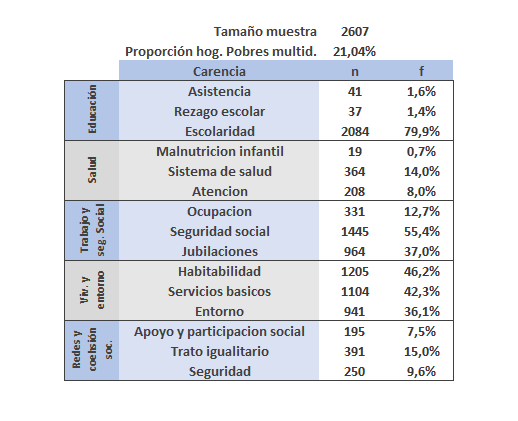
\includegraphics[height=9cm]{HOGARES/tabla_num2.png}
        \caption{Frecuencia de carencias Hogares de 2 integrantes. Fuente: Elaboración propia.}
        \label{fren2}
    \end{figure}

    \begin{figure}[H]
        \centering
        \includegraphics[width=\textwidth]{Mati N/n=2.png}
        \caption{Tipologías más frecuentes Hogares de 2 integrantes. Fuente: Elaboración propia.}
        \label{tipn2}
    \end{figure}

    Las carencias más frecuentes son Escolaridad (79,9\%), Seguridad social (55,4\%) y las carencias de la dimensión de Vivienda y entorno. Mientras que las carencias menos frecuentes son Malnutrición infantil, Rezago escolar y Asistencia escolar. 

    Los hogares pobres multidimensionales de 2 integrantes presentan 549 tipologías de carencias. Dentro de las 10 tipologías más frecuentes, que representan el 35,86\% del subgrupo, Escolaridad y las carencias de la dimensión Vivienda y entorno son las que tienen mayor incidencia, y las dimensiones Salud y Redes y cohesión social no presentan ninguna privación. 
    
    \item \textbf{Hogares de 3 integrantes}
    
    El subgrupo de hogares pobres multidimensionales de 3 integrantes reúne a 2.681 hogares, que representan 21,63\% de los hogares pobres multidimensionales. En las Figuras \ref{fren3} y \ref{tipn3} se presentan las frecuencias y tipologías de las carencias respectivamente.
    
    \begin{figure}[H]
        \centering
        \includegraphics[height=9cm]{HOGARES/tabla_num3.png}
        \caption{Frecuencia de las carencias Hogar de 3 integrantes. Fuente: Elaboración propia.}
        \label{fren3}
    \end{figure}

    \begin{figure}[H]
        \centering
        \includegraphics[width=\textwidth]{Mati N/n=3.png}
        \caption{Tipologías más frecuentes Hogar de 3 integrantes. Fuente: Elaboración propia.}
        \label{tipn3}
    \end{figure}
    
    Escolaridad, Seguridad social y Habitabilidad son las carencias más frecuentes en este tipo de hogar, con frecuencias de 73,6\%, 64,7\% y 51,1\% respectivamente. Las carencias menos frecuentes son Rezago escolar, Asistencia escolar y Apoyo y participación social.
    
    Los hogares pobres multidimensionales de 3 integrantes presentan 745 tipologías. Dentro de las 10 tipologías más frecuentes, que representan el 25,89\% de la submuestra, resulta importante destacar la incidencia de Escolaridad y Seguridad social, la inexistencia de carencias de la dimensión Redes y cohesión social, y la aparición de la carencia Adscripción a sistema de salud.
    
    \item \textbf{Hogares de 4 integrantes}
    
    El subgrupo de hogares pobres multidimensionales de 4 integrantes comprende 2.305 hogares, que representan el 18,6\% del total de hogares pobres multidimensionales. En las Figuras \ref{fren4} y \ref{tipn4} se presentan las frecuencias y tipologías de las carencias respectivamente.
   
    \begin{figure}[H]
        \centering
        \includegraphics[height=9cm]{HOGARES/tabla_num4.png}
        \caption{Frecuencia de las carencias Hogar de 4 integrantes. Fuente: Elaboración propia.}
        \label{fren4}
    \end{figure}
    \begin{figure}[H]
        \centering
        \includegraphics[width=\textwidth]{Mati N/n=4.png}
        \caption{Tipologías más frecuentes Hogar de 4 integrantes. Fuente: Elaboración propia.}
        \label{tipn4}
    \end{figure}
    
    Escolaridad y Seguridad social son las carencias más frecuentes, mientras que Apoyo y participación social, Rezago escolar y Atención de salud son las que tienen menor frecuencia.
    
    Los hogares pobres multidimensionales de 4 integrantes presentan 803 tipologías de carencias, de las cuales las 10 más frecuentes representan el 20,52\% de la submuestra. De las tipologías más frecuentes destaca la incidencia de las carencias Escolaridad y Seguridad social, la inexistencia de carencias de la dimensión Redes y cohesión social, y los \textit{IPM} en el margen con la mínima cantidad de carencias para ser considerados pobres multidimensionales.
    
    \item \textbf{Hogares de 5 integrantes}
    
    El subgrupo de hogares pobres multidimensionales de 5 integrantes reúne 1.780 hogares, que representan el 14,36\% del total de hogares pobres. En las Figuras \ref{fren5} y \ref{tipn5} se muestran las frecuencias y tipologías de la carencias respectivamente.
    
    \begin{figure}[H]
        \centering
        \includegraphics[height=9cm]{HOGARES/tabla_num5.png}
        \caption{Frecuencia de las carencias Hogares de 5 integrantes. Fuente: Elaboración propia.}
        \label{fren5}
    \end{figure}
    \begin{figure}[H]
        \centering
        \includegraphics[width=\textwidth]{Mati N/n=5.png}
        \caption{Tipologías más frecuentes Hogar de 5 integrantes. Fuente: Elaboración propia.}
        \label{tipn5}
    \end{figure}
    Escolaridad y Seguridad social son las carencias con mayor frecuencia, mientras que Atención de salud y Apoyo y participación social son las menos frecuentes.
    
    Este subgrupo presenta 663 tipologías de carencias, de las cuales las 10 más frecuentes representan el 21,8\% del total de hogares de la submuetsra. Dentro de las tipologías más frecuentes destaca la incidencia de las carencias Escolaridad, Seguridad social y Habitabilidad, la manifestación de carencias de las dimensiones Salud y Redes y cohesión social, y la existencia de 4 tipologías que reúnen 4 carencias simultáneas. 
    
    \item \textbf{Hogares de 6 integrantes}
    
    El subgrupo de hogares pobres multidimensionales de 6 integrantes tiene un tamaño de 911 hogares, que equivale al 7,35\% de la muestra. Las Figuras \ref{fren6} y \ref{tipn6} muestran las frecuencias de las carencias y las tipologías respectivamente.
    
    \begin{figure}[H]
        \centering
        \includegraphics[height=9cm]{HOGARES/tabla_num6.png}
        \caption{Frecuencia de las carencias Hogares de 6 integrantes. Fuente: Elaboración propia.}
        \label{fren6}
    \end{figure}
    \begin{figure}[H]
        \centering
        \includegraphics[width=\textwidth]{Mati N/n=6.png}
        \caption{Tipologías más frecuentes Hogar de 6 integrantes. Fuente: Elaboración propia.}
        \label{tipn6}
    \end{figure}
    Escolaridad, Seguridad social y Habitabilidad son las carencias con mayor frecuencia, mientras que Atención de salud y Apoyo y participación social son las carencias con menor frecuencia.
    
    Los hogares pobres multidimensionales de 6 integrantes reúnen 469 tipologías, donde las 10 más frecuentas representan el 19,76\% de la submuestra. Dentro de las tipologías más frecuentes destaca la incidencia de Escolaridad y Seguridad social, y la inexistencia de carencias de la dimensión Redes y cohesión social.

    \item \textbf{Hogares de 7 o más integrantes}
    
    El subgrupo de hogares pobres multidimensionales de 7 o más integrantes contiene 862 hogares, que representan el 6,96\% del total de hogares pobres. En las Figuras \ref{fren7} y \ref{tipn7} se muestran las frecuencias de las carencias y las tipologías respectivamente.
    
    \begin{figure}[H]
        \centering
        \includegraphics[height=9cm]{HOGARES/tabla_num7.png}
        \caption{Frecuencia de las carencias Hogares de 7 o más integrantes. Fuente: Elaboración propia.}
        \label{fren7}
    \end{figure}
    \begin{figure}[H]
        \centering
        \includegraphics[width=\textwidth]{Mati N/n=7+.png}
        \caption{Tipologías más frecuentes Hogar de 7 o más integrantes. Fuente: Elaboración propia.}
        \label{tipn7}
    \end{figure}
    Escolaridad, Seguridad social y Habitabilidad son las carencias con mayor frecuencia, mientras que Atención de salud y Apoyo y participación social son las carencias con menor frecuencia.
    
    Este subgrupo de hogares reúne 494 tipologías de pobreza. Dentro de las 10 tipologías más frecuentes, que representan el 16,47\% de la submuestra, destaca la incidencia de las carencias Escolaridad y Seguridad social, y la existencia de 4 tipologías que reúnen 4 carencias simultáneas.

\end{itemize}

\subsubsection{Análisis tipológico por zona de residencia}
La descomposición de la muestra por zona de residencia generó 2 subgrupos, que fueron analizados considerando las frecuencias tipologías de las carencias. A continuación, se detallan los resultados para cada subgrupo.

\begin{itemize}
    \item \textbf{Hogares Urbanos}
    
    El subgrupo de hogares pobres multidimensionales urbanos reúne 7.649 hogares, que equivalen al 61,73\% del total de hogares pobres. En las Figuras \ref{frenU} y \ref{tipnU} se presentan las frecuencias y tipologías de las carencias respectivamente. 
    
    \begin{figure}[H]
        \centering
        \includegraphics[height=9cm]{HOGARES/tabla_urbano.png}
        \caption{Frecuencias de las carencias Hogares Urbanos. Fuente: Elaboración propia.}
        \label{frenU}
    \end{figure}
    \begin{figure}[H]
        \centering
        \includegraphics[width=\textwidth]{Mati N/Urbano.png}
        \caption{Tipologías más frecuentes Hogares Urbanos. Fuente: Elaboración propia.}
        \label{tipnU}
    \end{figure}
    
    Escolaridad, Seguridad social y Habitabilidad son las carencias más frecuentes, mientras que Rezago escolar, Asistencia escolar, Apoyo y participación social y Atención de salud son las carencias menos frecuentes.
    
    Los hogares pobres multidimensionales urbanos presentan 1.552 tipologías, donde las 10 más frecuentes representan el 20,87\% de la submuestra. Dentro de las tipologías más frecuentes destaca la incidencia de las carencias Escolaridad, Seguridad social y Habitabilidad, la baja incidencia de las dimensiones Salud y Redes y cohesión social, y los \textit{IPM} en el margen con 3 carencias simultáneas en 9 de las 10 tipologías.
    
    \item \textbf{Hogares Rurales}
    
    El subgrupo de hogares pobres multidimensionales rurales contiene 4.743 hogares, que equivalen al 38,27\% del total de hogares pobres multidimensionales. En las Figuras \ref{freU} y \ref{tipR} se presentan las frecuencias y tipologías de las carencias respectivamente. 
    
    \begin{figure}[H]
        \centering
        \includegraphics[height=9cm]{HOGARES/tabla_rural.png}
        \caption{Frecuencias de las carencias Hogares Rurales. Fuente: Elaboración propia.}
        \label{freU}
    \end{figure}
    \begin{figure}[H]
        \centering
        \includegraphics[width=\textwidth]{Mati N/Rural.png}
        \caption{Tipologías más frecuentes Hogares Rurales. Fuente: Elaboración propio.}
        \label{tipR}
    \end{figure}
    Escolaridad, Servicios básicos y Seguridad social son las carencias más frecuentes, mientras que Seguridad, Atención de salud, Rezago escolar y Apoyo y participación social son las carencias menos frecuentes.
    
    Este subgrupo presenta 769 tipologías, donde las 10 más frecuentes representan el 37,66\% de la submuestra. Dentro de las tipologías más frecuentes, Escolaridad, Servicios básicos y Habitabilidad son las carencias con mayor incidencia, mientras que las carencias de las dimensiones de Salud y Redes y cohesión social no tienen incidencia. 
    
\end{itemize}





%%%%%%%%%%%%%%%%%%%%%%%%%%%%%%%%%%%%%%%%%%%%%%%%%%%%% RESULTADOS MAX 
\subsubsection{Análisis comparativo con nivel de ingresos}


Para obtener el indicador de ingreso relativo a la línea de pobreza, se emplearon los valores del ingreso autónomo del hogar ajustado per cápita (\textit{ypc}) de los hogares pobres multidimensionales de la muestra, y los valores de le línea de la pobreza (LP) ajustada según número de personas que componen el hogar en Noviembre de 2017 (Fig. \ref{LPLPE}). Considerando la disponibilidad de valores de LP ajustada para hogares conformados entre 1 y 10 personas, para el análisis comparativo con el nivel de ingreso se consideraron sólo aquellos hogares pobres multidimensionales de 1 a 10 integrantes, y para los que se contara con el valor de \textit{ypc}, conjunto conformado por 12.363 hogares, que corresponden al 99.8\% de los hogares pobres multidimensionales de la muestra.


Habiéndose clasificado los hogares según estrato socio-económico, se puede evidenciar que los hogares que componen la clase media, en su conjunto, tienen la mayor contribución al total de hogares pobres multidimensionales (fig. \ref{distribucion_socio_pobres}), con una frecuencia acumulada de 54.6\%. Sin embargo, esta contribución se explica en su mayor parte por el total de hogares pertenecientes a la categoría \text(Clase media baja) (42.7\%). En orden de frecuencia, le siguen los hogares \textit{Vulnerables} y \textit{Pobres}, con frecuencias 25.7\% y 18.1\% respectivamente. Si bien el 86.4\% de los hogares pobres multidimensionales pertenecen a las categorías de menor ingreso (\textit{pobres}, \textit{vulnerables} y \textit{clase media baja}, el aporte de un 13.6\% de los hogares con mayores ingresos permite determinar que el fenómeno de la pobreza multidimensional no es exclusivamente propio de los hogares con menores ingresos.

\begin{figure}[H]
    \centering
    \includegraphics[height=8 cm]{Max/distribucion_pobres_clase.png}
    \caption{Distribución de pobres multidimensionales por clasificación socio-económica. Fuente: elaboración propia.}
    \label{distribucion_socio_pobres}
\end{figure}


Sin embargo, la distribución de los hogares pobres multidimensionales en estas 6 categorías se puede explicar por la distribución del total de hogares (pobres y no pobres) dentro de ellas. Como se puede apreciar en la figura \ref{distribucion_socio}, existe una distribución similar en el total de hogares, siendo particular el caso de los hogares clasificados como \textit{Clase. M. Baja} con una diferencia de 0.5\%. A partir de proporcionalidad directa se podría inferir que la prevalencia porcentual de la pobreza multidimensional se puede traducir directamente como la probabilidad de un hogar de clase media baja de ser pobre dimensional.

\begin{figure}[!]
    \centering
    \includegraphics[height=8 cm]{Max/clasificacione_social_general.png}
    \caption{Distribución de hogares por clasificación socio-económica. Fuente: elaboración propia.}
    \label{distribucion_socio}
\end{figure}


En términos de la prevalencia porcentual de la pobreza multidimensional relativa al total de hogares en cada categoría (fig. \ref{distribucion_relativa}, se puede evidenciar claramente que, en la medida en que el nivel de ingresos del hogar es mayor, disminuye la probabilidad de ser clasificado como pobre dimensional. 


\begin{figure}[!]
    \centering
    \includegraphics[height=8 cm]{Max/tipos_prop.png}
    \caption{Distribución de pobreza multidimensional por clasificación socio-económica. Fuente: elaboración propia.}
    \label{distribucion_relativa}
\end{figure}


Si bien este análisis de la composición socio-económica (en función del criterio empleado) nos permite determinar que la probabilidad de un hogar de ser clasificado como pobre dimensional se relaciona de forma inversa a su nivel de ingresos, es necesario determinar la relación entre la intensidad de la pobreza multidimensional, expresada en el valor del \textit{IPM}, y el nivel de ingresos de los hogares (fig. \ref{scatter_general_quiebre}). A pesar de que valores más altos del \textit{IPM} tienen asociados menores niveles de ingreso, la alta concentración de datos en torno a los valores menores del \textit{IPM} permite inferir que la distribución del ingreso de los hogares en función del \textit{IPM} (fig. \ref{res_frec} no sigue un patrón lineal, lo cual queda comprobado con el cálculo del coeficiente de Pearson entre ambas variables \textit{r=-0,09004}, que nos indica una relación lineal insignificante entre ambas variables (fig. \ref{res_frec}).


\begin{figure}[!]
    \centering
    \includegraphics[width=\textwidth]{Max/scatter_General_quiebre.png}
    \caption{Dispersión del ingreso de hogares pobres multidimensionales, expresado en proporción al valor de LP, respecto al \textit{IPM}. Fuente: elaboración propia.}
    \label{scatter_general_quiebre}
\end{figure}

\begin{figure}[!]
    \centering
    \includegraphics[width=\textwidth]{Max/resumen_frecuencias_IPM.png}
    \caption{Resumen frecuencia de valores \textit{IPM}, hogares pobres multidimensionales. Fuente: elaboración propia.}
    \label{res_frec}
\end{figure}




%%%%%%%%%%%%%%%%%%%%%%%%%%%%%%%%%%%%%%%%%%%%%%%%%%%%%%%% RESULTADOS TIPOLOGÍAS POR CLASE

\begin{figure}[H]
    \centering
    \includegraphics[width=\textwidth]{Max/tipol_pobres.png}
    \caption{Tipologías de carencias más frecuentes de los hogares pobres multidimensionales y pobres por ingreso. Fuente: Elaboración propia.}
    \label{TipPob}
\end{figure}

\begin{figure}[H]
    \centering
    \includegraphics[width=\textwidth]{Max/tipol_vulnerables.png}
    \caption{Tipologías de carencias más frecuentes de los hogares pobres multidimensionales y vulnerables por ingreso. Fuente: Elaboración propia.}
    \label{TipVul}
\end{figure}

\begin{figure}[H]
    \centering
    \includegraphics[width=\textwidth]{Max/tipol_CMB.png}
    \caption{Tipologías de carencias más frecuentes de los hogares pobres multidimensionales y clase media baja. Fuente: Elaboración propia.}
    \label{TipCMB}
\end{figure}

\begin{figure}[H]
    \centering
    \includegraphics[width=\textwidth]{Max/tipol_CMM.png}
    \caption{Tipologías de carencias más frecuentes de los hogares pobres multidimensionales y clase media media. Fuente: Elaboración propia.}
    \label{TipCMM}
\end{figure}

\begin{figure}[H]
    \centering
    \includegraphics[width=\textwidth]{Max/tipol_CMA.png}
    \caption{Tipologías de carencias más frecuentes de los hogares pobres multidimensionales y clase media alta. Fuente: Elaboración propia.}
    \label{TipCMA}
\end{figure}

\begin{figure}[H]
    \centering
    \includegraphics[width=\textwidth]{Max/tipol_AI.png}
    \caption{Tipologías de carencias más frecuentes de los hogares pobres multidimensionales y de altos ingresos. Fuente: Elaboración propia.}
    \label{TipAI}
\end{figure}



%%%%%%%%%%%%%%%%%%%%%%%%%%%%%%%%%%%%%%%%%%%%%%%%%%%%%% FIN RESULTADOS TIPOLOGÍAS POR CLASE






Con el objetivo de realizar un análisis más específico del nivel de ingreso en al la intensidad de la pobreza multidimensional, se definieron 5 intervalos que agrupan  (\textit{Tabla frecuencia IPM por intervalos} fig. \ref{res_frec}) la muestra de hogares pobres multidimensionales según su \textit{IPM}. Si bien se puede apreciar que, cuando emplea como referencia la distribución general (fig. \ref{box_general}, la distribución del ingreso por los intervalos presenta poca variación,  aquel constituido por los hogares con mayor ponderación de \textit{IPM}  es también el que presenta menor dispersión en relación al ingreso, encontrándose más del 25\% de estos hogares bajo la línea de la pobreza, y más del 50\% bajo la línea de vulnerabilidad. 

\begin{figure}[!]
    \centering
    \includegraphics[height=10 cm]{Max/box_general.png}
    \caption{Distribución ingreso, expresado en en proporción al valor de LP, hogares pobres multidimensionales. Fuente: elaboración propia.}
    \label{box_general}
\end{figure}


\begin{figure}[!]
    \centering
    \includegraphics[width=\textwidth]{Max/box_deciles2.png}
    \caption{Distribución ingreso expresado en en proporción al valor de LP por intervalos de \textit{IPM}, hogares pobres multidimensionales. Fuente: elaboración propia.}
    \label{box_deciles}
\end{figure}



Finalmente, habiéndose realizado un análisis de la distribución del ingreso entre aquellos hogares pobres que padecen una carencia en particular (análisis realizado para cada una de las 15 carencias del modelo de 15 dimensiones, \ref{box_carencias}), se puede observar que las 3 carencias cuya prevalencias están asociadas a hogares pobres multidimensionales con mayor dispersión del nivel de ingresos, son las carencias \textit{adscripción a sistema de salud} y \textit{atencón} (dimensión \textit{Salud}), y la carencia \textbf{Jubilaciones} (dimensión \textit{Trabajo y seguridad social}).



\begin{figure}[!]
    \centering
    \includegraphics[width=\textwidth]{Max/box_carencias.png}
    \caption{Distribución ingreso expresado en en proporción al valor de LP, por hogares pobres multidimensionales con presencia de cada carencia. Fuente: elaboración propia.}
    \label{box_carencias}
\end{figure}
%%%%%%%%%%%%%%%%%%%%%%%%%%%%%%%%%%%%%%%%%%%%%%%%% FIN RESULTADOS MAX

\subsection{RESULTADOS PARTE III}


\subsubsection{Análisis de sensibilidad}




\begin{figure}[H]
    \centering
        \includegraphics[width=11cm]{Max/estadistica_escenario.png}
    \caption{Resumen resultados frecuencia hogares pobres multidimensionales, escenario alternativo para el cálculo del \textit{IPM}. Fuente: elaboración propia.}
    \label{resusensible}
\end{figure}


\begin{figure}[H]
    \centering
        \includegraphics[width=\textwidth]{Max/Heatmap_pearson_Escenario_sensibilidad_1.png}
    \caption{Correlación entre carencias hogares pobres, escenario alternativo para el cálculo del \textit{IPM}. Fuente: elaboración propia.}
    \label{heatmap_sensible}
\end{figure}


\begin{figure}[H]
    \centering
        \includegraphics[width=14cm]{Max/variacion_correlaciones.png}
    \caption{Variacion negativo positivo. NO se si mantener. Fuente: elaboración propia.}
    \label{varposneg}
\end{figure}





\subsubsection{Proyecciones IPM }

El período de referencia para las proyecciones que se realizarán a continuación corresponde al de recopilación de datos de la encuesta CASEN 2017 (noviembre 2017 - febrero 2018). En función de lo anterior, la tasa de desocupación referencial seleccionada corresponde a la del trimestre móvil \textit{noviembre 2017 - enero 2018} (AGREGAR REFERENCIA INE), estimada en un 6.5\%. El indicador de seguridad\footnote{El indicador de seguridad empleado corresponde al índice porcentual de Percepción del aumento de la delincuencia y exposición frente al delito}, será el correspondiente al estimado por el \textit{INE} a través de la \textit{ENUSC} para el año 2017, el cual corresponde a un 45.2\%. 

En cuanto a los indicadores asociados al período proyectado (Junio de 2020), se emplearán en primera instancia las últimas estimaciones de la tasa de desocupación y del indicador de seguridad de la \textit{ENUSC} a la fecha de realización del presente estudio. Para el caso de la tasa de desocupación, se empleará el valor estimado por el \textit{INE} para el trimestre móvil marzo - mayo 2020, el cual corresponde a 11.2\%; para el caso del indicador de seguridad de la \textit{ENUSC} se empleará el estimado en el boletín correspondiente al año 2019. el cual corresponde a 39.02\%.

Sin embargo, considerando el escenario actual de crisis sanitaria asociada a la pandemia COVID-19, y a las  profundas consecuencias que ha implicado en el desarrollo de las actividades habituales de la población, el indicador de seguridad de la \textit{ENUSC} 2019 se encuentra obsoleto. Ante lo anterior, surge la necesidad de emplear una nueva estimación que recoja una impresión actualizada de la realidad nacional. En el contexto del proyecto \textit{Monitor de Seguridad}, desarrollado por la \textit{Fundación Chile 21}, se ha realizado en junio de 2020 la encuesta \textit{Seguridad Ciudadana y Evaluación Policial}\footnote{Disponible en el sitio web INSERTAR ACA SITIO WEB. Los resultados de esta encuesta han sido ponderados de acuerdo a la distribución socio-demográfica de Chile, determinada en la encuesta CASEN 2017 y del Censo 2017.} (\textit{ESCEP}), entre cuyos resultados se dispone de un indicador porcentual de la percepción del delito (venta de drogas y balaceras) en el sector de residencia (fig. \ref{monitor}), que es coherente con la medida empleada para el cálculo del indicador de la carencia \textit{seguridad} (fig. \ref{criterios}). Si se supone, por lo tanto, que la incidencia de la carencia \textit{seguridad} es proporcional entre el total de personas y el total de hogares, se podría realizar una estimación directa de la distribución de la carencia. y la frecuencia de percepción de los delitos. No obstante, debido a que no se dispone de los datos relativos a simultaneidad en la percepción de ambos delitos, se pueden inferir dos escenarios extremos: 

\begin{itemize}
    
    \item La intersección entre el conjunto de personas que perciben una alta frecuencia de venta de drogas en su sector (frecuencia estimada en un 48\%), y el conjunto de personas que perciben una alta frecuencia de balaceras en su sector (frecuencia estimada en un 28\%), es igual a 0. Ello implicaría que la distribución de la carencia \textit{seguridad} correspondería a la suma de ambas frecuencias: 76\% (escenario menos conservador). 
    

    \item El conjunto de personas que perciben una alta frecuencia de balaceras en su sector es un subconjunto del conjunto de personas que perciben una alta frecuencia de venta de drogas en su sector. Ello implicaría que la distribución de la carencia \textit{seguridad} correspondería a la frecuencia del conjunto de personas que perciben una alta frecuencia de venta de drogas: 48\% (escenario más conservador).
    
    \end{itemize}




\begin{figure}[H]
    \centering
    \includegraphics[width=\textwidth]{Max/monitor_seguridad_2.png}
    \caption{Percepción frecuencia exposición a venta de drogas y a balaceras o disparos. Fuente: Monitor de Seguridad (2020). Encuesta Seguridad Ciudadana y Evaluación Policial.}
    \label{monitor}
\end{figure}




La \textit{CEPAL}, a su vez, ha realizado una proyección de la tasa de desempleo en América Latina y el Caribe para el 2020, en función de la declinación de la actividad económica producto de la pandemia (INSERTAR CITA CEPAL), previendo un mínimo de 11.5\%. La proyección de los datos realizados en el presente estudio, por lo tanto, contempla también el escenario en el cual la tasa de desocupación de Chile alcance el nivel proyectado por la \textit{CEPAL}.



En virtud de lo anterior, se realizaron 5 proyecciones del Indicador de Pobreza Multidimensional, efectuadas en base a 5 escenarios posibles según los diferentes estimadores empleados:

\begin{itemize}
\item \textbf{Escenario 1:} Proyección realizada sobre la estimación de la tasa de desocupación del trimestre móvil marzo-mayo 2020 (\textit{INE}) e indicador de seguridad \textit{ENUSC}.

\item \textbf{Escenario 2:} Proyección realizada sobre la estimación de la tasa de desocupación del trimestre móvil marzo-mayo 2020 (INE) e indicador de seguridad más conservador obtenido de la \textit{ESCEP}.	

\item \textbf{Escenario 3:} Proyección realizada sobre la estimación de la tasa de desocupación del trimestre móvil marzo-mayo 2020 (INE) e indicador de seguridad menos conservador obtenido de la \textit{ESCEP}.

\item \textbf{Escenario 4:} Proyección realizada sobre la estimación de la tasa de desocupación América Latina y el Caribe (\textit{CEPAL}) e indicador de seguridad más conservador obtenido de la \textit{ESCEP}.	

\item \textbf{Escenario 5:} Proyección realizada sobre la estimación de la tasa de desocupación América Latina y el Caribe (\textit{CEPAL}) e indicador de seguridad menos conservador obtenido de la \textit{ESCEP}.


\end{itemize}

En la figura \ref{resumen_ind_escenarios} se puede observar un resumen de los indicadores empleados, así como la distribución estimada de las carencias \textit{ocupación} y \textit{seguridad}, para cada uno de los escenarios. 


\begin{figure}[H]
    \centering
    \includegraphics[width=\textwidth]{Max/resumen_escenarios.png}
    \caption{Resumen de los indicadores empleados en los distintos escenarios de proyección. Fuente: elaboración propia.}
    \label{resumen_ind_escenarios}
\end{figure}

En base a las frecuencias de \textit{ocupación} y \textit{seguridad} proyectadas en cada escenario, se estimaron los parámetros de distribución \textit{Bernoulli} para la generación de datos aleatorios de las variables $ocupacion_j$ y $seguridad_j$ (fig. \ref{parametros_pq}). Para cada escenario de simulación se efectuó un total de 1000 iteraciones, realizándose la proyección de las medidas de desempeño en base al promedio obtenido de las observaciones realizadas. Como se puede observar en las figuras \ref{escenario_1}, \ref{escenario_2}, \ref{escenario_3}, \ref{escenario_4} y \ref{escenario_5}, en la medida en que aumenta el número de iteraciones en cada escenario de simulación, el promedio de las observaciones realizadas converge en torno a un valor, pudiéndose evidenciar que para todos los experimentos realizados, se obtiene un valor promedio estable antes de las 1000 iteraciones.


\begin{figure}[H]
    \centering
    \includegraphics[width=\textwidth]{Max/parametros_bernoulli.png}
    \caption{Parámetros estimados para la distribución de variables aleatorias en los modelos de entrada de cada escenario. Fuente: elaboración propia.}
    \label{parametros_pq}
\end{figure}






\begin{figure}[H]
    \centering
    \includegraphics[width=\textwidth]{Max/grafico_ENUSC_Escenario1.png}
    \caption{Valores promedio observados para cada medida de desempeño, en función del número de iteraciones, \textit{Escenario 1}. Fuente: elaboración propia.}
    \label{escenario_1}
\end{figure}

\begin{figure}[H]
    \centering
    \includegraphics[width=\textwidth]{Max/grafico_MONITOR_OP_Escenario2.png}
    \caption{Valores promedio observados para cada medida de desempeño, en función del número de iteraciones, \textit{Escenario 2}. Fuente: elaboración propia.}
    \label{escenario_2}
\end{figure}

\begin{figure}[H]
    \centering
    \includegraphics[width=\textwidth]{Max/grafico_MONITOR_PES_Escenario3.png}
    \caption{Valores promedio observados para cada medida de desempeño, en función del número de iteraciones, \textit{Escenario 3}. Fuente: elaboración propia.}
    \label{escenario_3}
\end{figure}


\begin{figure}[H]
    \centering
    \includegraphics[width=\textwidth]{Max/grafico_CEPAL_OP_Escenario4.png}
    \caption{Valores promedio observados para cada medida de desempeño, en función del número de iteraciones, \textit{Escenario 4}. Fuente: elaboración propia.}
    \label{escenario_4}
\end{figure}


\begin{figure}[H]
    \centering
    \includegraphics[width=\textwidth]{Max/grafico_simulacion_CEPAL_PES_Escenario5.png}
    \caption{Valores promedio observados para cada medida de desempeño, en función del número de iteraciones, \textit{Escenario 5}. Fuente: elaboración propia.}
    \label{escenario_5}
\end{figure}

En la figura \ref{resumen_resultados_escenarios} se puede observar un resumen de las estimaciones realizadas para cada escenario. 






\begin{figure}[H]
    \centering
    \includegraphics[width=\textwidth]{Max/resultados_escenarios.png}
    \caption{Resumen de resultados de la proyección de la pobreza multidimensional en Chile. Fuente: elaboración propia.}
    \label{resumen_resultados_escenarios}
\end{figure}

















\newpage
\section{Conclusiones} % 5 puntos






% Bibliografia 
\newpage
\addcontentsline{toc}{section}{Referencias}
\bibliographystyle{apalike}
\bibliography{references}


% Anexos 
\newpage
 \vspace*{\fill}
\section*{\centering Anexos}\addcontentsline{toc}{section}{Anexos}
 \vspace*{\fill}
\newpage


%%%%%%%%%%%%%%%%%%%%%%%%%%%%%%%%%%%%%%%%%%%%%%%%% CRITERIO DEFINICIÓN CARENCIAS CASEN 2017
\begin{figure}[H]
    \centering
        \includegraphics[height=\textheight]{Criterios carencias - Manual del investigador.png}
    \caption{Criterios medición pobreza multidimensional. Fuente: Manual del investigador CASEN 2017}
    \label{criterios}
\end{figure}
\newpage
%%%%%%%%%%%%%%%%%%%%%%%%%%%%%%%%%%%%%%%%%%%%%%%%% ANEXO DESCRIPCIÓN BASE DE DATOS
\section*{\centering Anexo 1: Descripción base de datos empleada}\addcontentsline{toc}{section}{Anexo1: Descripción base de datos empleada}\label{descripcion_base_datos}

La base de datos empleada para el estudio realizado constituye una modificación de la base de datos de la encuesta CASEN 2017 dispuesta para su uso público por el Ministerio de Desarrollo Social y Familia del Gobierno de Chile\footnote{La base de datos original puede ser descargada desde el sitio \url{http://observatorio.ministeriodesarrollosocial.gob.cl/casen-multidimensional/casen/basedatos.php} en formatos STATA y SPSS}. Dichas modificaciones se efectuaron con el fin de facilitar su manipulación para el desarrollo de análisis con las herramientas de programación disponibles. A continuación se indican las modificaciones realizadas:

\begin{enumerate}
    \item \textbf{Selección de atributos}
    En la encuesta original, a cada persona encuestada se le describe con un total de 804 atributos, los que corresponden tanto a datos individuales, como a datos compartidos por los miembros de la vivienda, el hogar y el núcleo familiar. De estos atributos se seleccionaron 47. En la figura \ref{atributos} se indican los atributos con su respectiva definición, además de su ubicación en la base de datos original (empleando como referencia los indicadores de columnas en formato CVS). 
    
    \item \textbf{Redenominación de atributos}
    Se redenominaron los atributos asociados a los indicadores dicotómicos de las carencias, como lo indica la figura \ref{redenominacion}.
    
    \item \textbf{Revalorización de atributo pco1}
    El atributo \textit{pco1} indica la relación de la persona encuestada con la persona designada como Jefe(a) de hogar. Los valores fueron modificados con indicadores numerales para cada tipo de relación, como lo indica la figura \ref{pco1}.
    
    \item \textbf{Revalorización de atributo pco2}
    El atributo \textit{pco2} indica la relación de la persona encuestada con la persona designada como Jefe(a) de Núcleo. Los valores fueron modificados con indicadores numerales para cada tipo de relación, como lo indica la figura \ref{pco2}.
    
\end{enumerate}

El resultado de estas modificaciones se encuentra disponible en el sitio \url{https://drive.google.com/file/d/1BZb8PdA50IijdIoJyVsBvS43jYxHCXYF/view?usp=sharing} en formato CVS. La estructura de datos resumida se puede observar en la figura \ref{estructura}


 \begin{figure} [H]
        \centering
        \includegraphics[height=\textheight]{atributos_casen.png}
        \caption{Atributos seleccionados. Fuente: elaboración propia.}
        \label{atributos}
    \end{figure}

    \begin{figure} [H]
        \centering
        \includegraphics{redenominacion.png}
        \caption{Redenominación de atributos. Fuente: elaboración propia.}
        \label{redenominacion}
    \end{figure}

    \begin{figure} [H]
        \centering
        \includegraphics{pco1.png}
        \caption{Revalorización atributo pco1. Fuente: elaboración propia.}
        \label{pco1}
    \end{figure}

    \begin{figure} [H]
        \centering
        \includegraphics{pco2}
        \caption{Revalorización atributo pco2. Fuente: elaboración propia.}
        \label{pco2}
    \end{figure}

\begin{figure} [H]
        \centering
        \includegraphics{estructura.png}
        \caption{Estructura de datos CASEN 2017 modificada. Fuente: elaboración propia.}
        \label{estructura}
    \end{figure}

\newpage
%%%%%%%%%%%%%%%%%%%%%%%%%%%%%%%%%%%%%%%%%%%%%%%%%%%%%%%%%%%%%%%%%%%%%%%%%%%%%

















\end{document}

%%%%\section*{Ejemplo sección sin número}\addcontentsline{toc}{section}{Nombre de la sección en índice}
%%%%% EJEMPLO COMILLAS ``comillas'' ``''
%%%%% EJEMPLO NÚMERO ORDINAL N\textordmasculine


%CONVERTIDOR FORMULAS A LATEX
% https://www.codecogs.com/latex/eqneditor.php 













